\documentclass[13pt]{beamer}
%\documentclass[handout]{beamer}
\usepackage{textcomp}
\usepackage{graphicx}
\usepackage{subfigure}
\usepackage{epsfig}
\usepackage{color}
\usepackage{amsmath,amsthm,amssymb,amsfonts,amsxtra,amstext}
\usepackage{pgf,pgfarrows,pgfnodes,pgfautomata,pgfheaps}
\usepackage[english]{babel}
\usepackage{mathptmx}
\usepackage{multimedia}
\usepackage{cancel}
\usepackage{hyperref}
\newcommand{\figdir}{../../fig}
\newcommand{\zap}[1]{ }
\newcommand{\xhat}{\hat{x}}
\newcommand{\sgn}{\mathrm{sgn}}
\renewcommand{\P}{\mathbb{P}}
\newcommand{\T}{\mathbb{T}} % Time index set.
\newcommand{\IZ}{\mathrm{IZ}}
\newcommand{\CS}{\mathrm{CS}}
\newcommand{\PZ}{\mathrm{PZ}}
\newcommand{\PCS}{\mathrm{PCS}}
% \newcommand{\R}{\mathbb{R}}
\newcommand{\Z}{\mathbb{Z}}
\newcommand{\Q}{\mathbb{Q}}
\newcommand{\Ybar}{\overline{Y}}
  \newcommand{\BIZ}{\mathrm{BIZ}}
  \newcommand{\sigmahat}{\widehat{\sigma}}
  \newcommand{\qhat}{\hat{q}}
\newcommand{\ceil}{\mathrm{ceil}}
\newcommand{\PstarB}{\mathcal{P}^*_B}
\newcommand{\upthresh}{P}

% Run with this to make it compile faster by leaving out the images
%\usepackage[draft]{graphics}

\input{../../evan_commands.tex}
\input{../../pete_commands.tex}

%\usetheme{Rochester}
%\usetheme{Antibes}
%\usetheme{Warsaw}
%\usetheme{Boadilla}
%\usetheme{Montpellier}
%\usetheme{Luebeck}
%\usetheme{Copenhagen}
%\usetheme{Malmoe}
%\usetheme{Pittsburgh}
%\usetheme{CambridgeUS}
%\usetheme{JuanLesPins}
%\usetheme{Luebeck}
%\usetheme{Marburg}
%\usetheme{Darmstadt}
%\usetheme{Berlin}
%\usetheme{PaloAlto}
%\usetheme{Dresden}
%\usetheme{Singapore}
%\usetheme{AnnArbor}
%\usetheme{Szeged}
%\usetheme{Berkeley}
%\usetheme{Bergen}
%\usetheme{Goettingen}
%\usetheme{Hannover}
%\usetheme{Ilmenau}
\usetheme{Madrid}
%\usetheme{Frankfurt}

%\usecolortheme{rose}
\usecolortheme{seahorse}
%\usecolortheme{sidebartab}
%\usecolortheme{IAS}
%\usecolortheme{crane}

%% If you have a file called "university-logo-filename.xxx", where xxx
%% is a graphic format that can be processed by latex or pdflatex,
%% resp., then you can add a logo as follows:
%
 %\pgfdeclareimage[height=0.5cm]{university-logo}{\figdir/cornell-logo.pdf}
 %\logo{\pgfuseimage{university-logo}}

\title{Optimal Learning:\\ Bayesian Methods for Simulation Optimization}
\author[Frazier]{Peter I. Frazier}
\institute[Cornell University]{Operations Research \& Information Engineering, Cornell University}
\date[talk]
{Thursday April 18, 2013\\ 
AFOSR Program Review\\
Optimization \& Discrete Mathematics\\
Arlington, VA\\
\vspace{0.2in}
AFOSR YIP FA9550-11-1-0083\\(Optimization \& Discrete Mathematics)\\
AFOSR BRI FA9550-12-1-0200, with Warren Powell\\(Natural Materials, Systems \& Extremophiles)
}

\AtBeginSection[]
{
   \begin{frame}
       \frametitle{Outline}
       \tableofcontents[currentsection]
   \end{frame}
}

\begin{document}

\setbeamertemplate{navigation symbols}{} %gets rid of navigation symbols
\setbeamertemplate{footline}{} % gets rid of footline

\frame{ \titlepage } % Make the title page

\zap{
\begin{frame} \frametitle{Overview}
  \begin{itemize}
    \item We use Bayesian statistics to design optimization algorithms for problems with expensive or time-consuming function evaluations.
    \item Objective functions are expensive or time-consuming to evaluate when they require running:
      \begin{itemize}
	\item a complex computer simulator; or
	\item a physical laboratory experiment.
      \end{itemize}
    \item We discuss two kinds of optimization algorithms:
      \begin{itemize}
	\item Methods with worst-case non-Bayesian guarantees on solution quality, where Bayesian analysis plays a role in the theory. 
	\item Methods with good (or even optimal) average-case (Bayesian) performance under the prior.
      \end{itemize}
  \end{itemize}
\end{frame}
}

\section{Part I: Worst-case Performance Guarantees}
\subsection{Ranking and Selection with Tight Bounds on Solution Quality}

% What is the problem?
\begin{frame} \frametitle{Ranking \& Selection (R\&S) is a basic problem in simulation optimization}
\begin{itemize}
  \item We have $k$ alternative choices that can be simulated.
  \item When we simulate alternative $x$, we observe random payoff $Z(x)$.
  \item We wish to know which $x$ has the largest $E[Z(x)]$.
  \item Sampling is the only way to estimate $E[Z(x)]$ because the simulator is too complex for direct theoretical analysis.  
    \begin{itemize}
      \item e.g., a large-scale discrete-event simulation of a supply chain; or a whole-theater combat simulator.
    \end{itemize}
  \item We make no a priori assumptions about the relationships between alternatives.
\end{itemize}
\end{frame}

\begin{frame} \frametitle{We Assume Independent Normal Samples}
  \begin{itemize}
  \item The R\&S literature often assumes that Z(x) is normally distributed: 
    \begin{equation*}
      Z(x) \sim \mathrm{Normal}(\theta_x, \sigma^2_x) \qquad \text{(independent across $x$ and time)}
    \end{equation*}
  \item $\theta_x$ is unknown but fixed (non-Bayesian). 
  \item For simplicity in this talk, we assume $\sigma^2_x$ is known, but the procedure presented can also be used in the unknown variance setting.
  \item Approximate normality of $Z(x)$ can be checked empirically, and if it is not met, samples can be batched together.
\end{itemize}
\end{frame}


\begin{frame} \frametitle{A Typical Ranking \& Selection Procedure}
  \begin{figure}
    \center 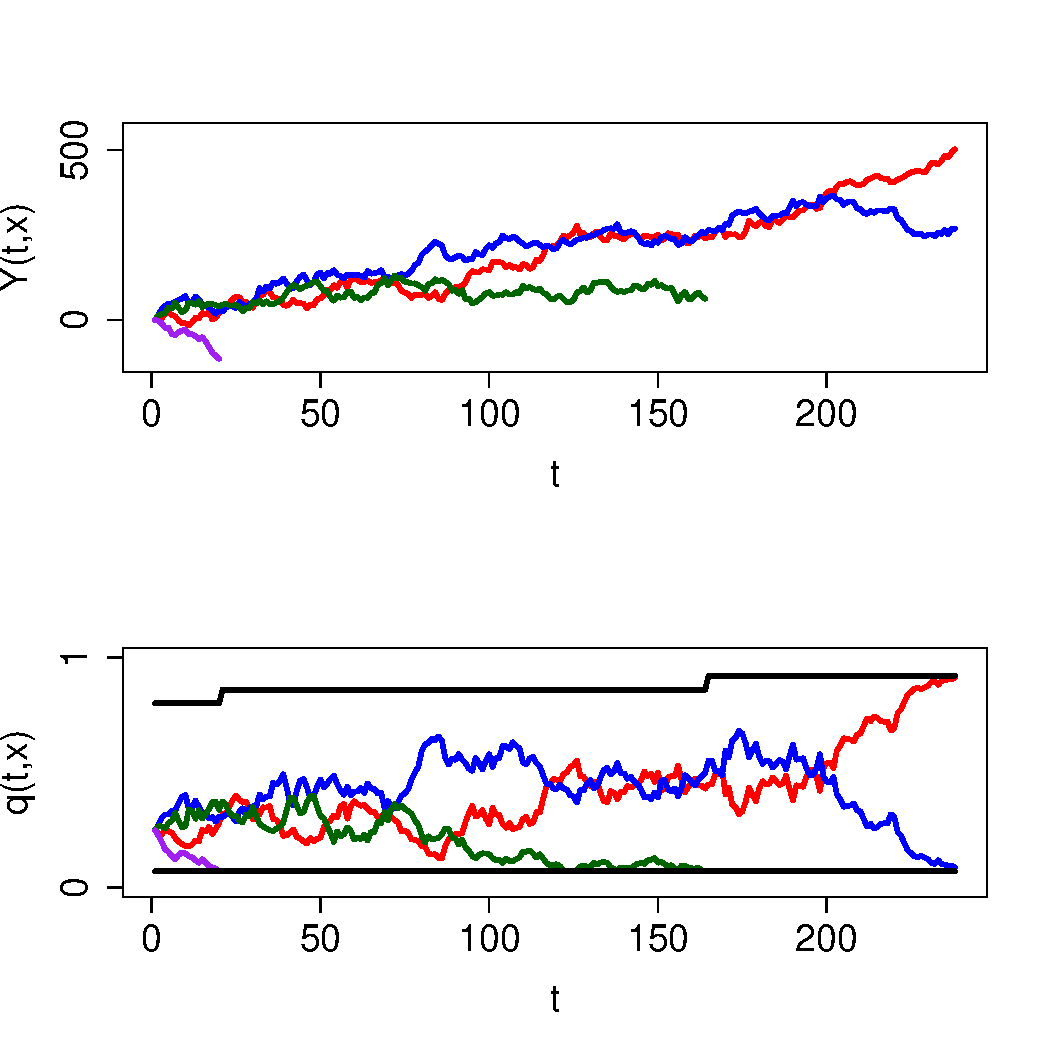
\includegraphics[height=\textheight]{\figdir/biz/AFOSR2013/animation/pdf2/animation_0238.pdf}
  \end{figure}
\end{frame}

\begin{frame}\frametitle{A Typical Ranking \& Selection Procedure}\begin{figure}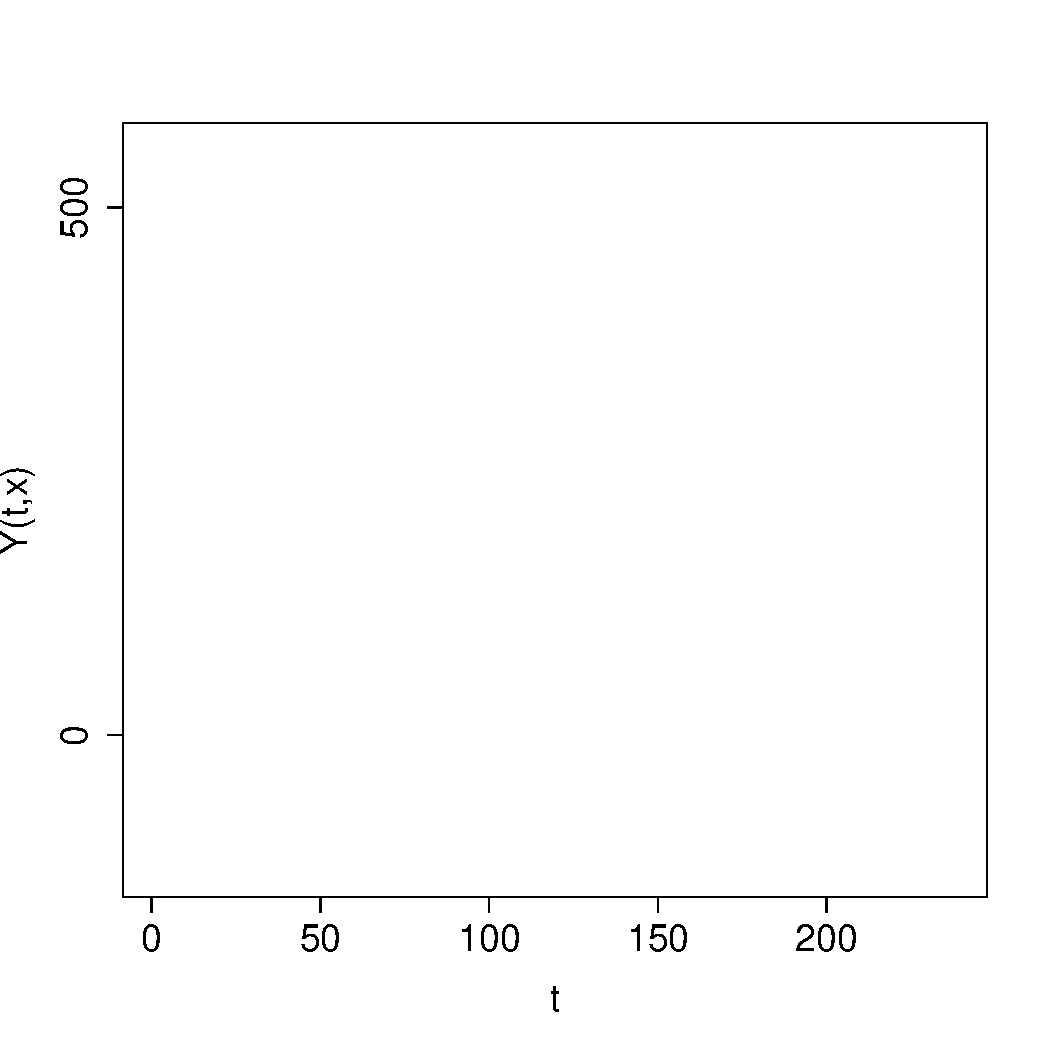
\includegraphics[height=\textheight]{\figdir/biz/AFOSR2013/animation/pdf2/animation_0001.pdf}\end{figure}\end{frame}
\begin{frame}\frametitle{A Typical Ranking \& Selection Procedure}\begin{figure}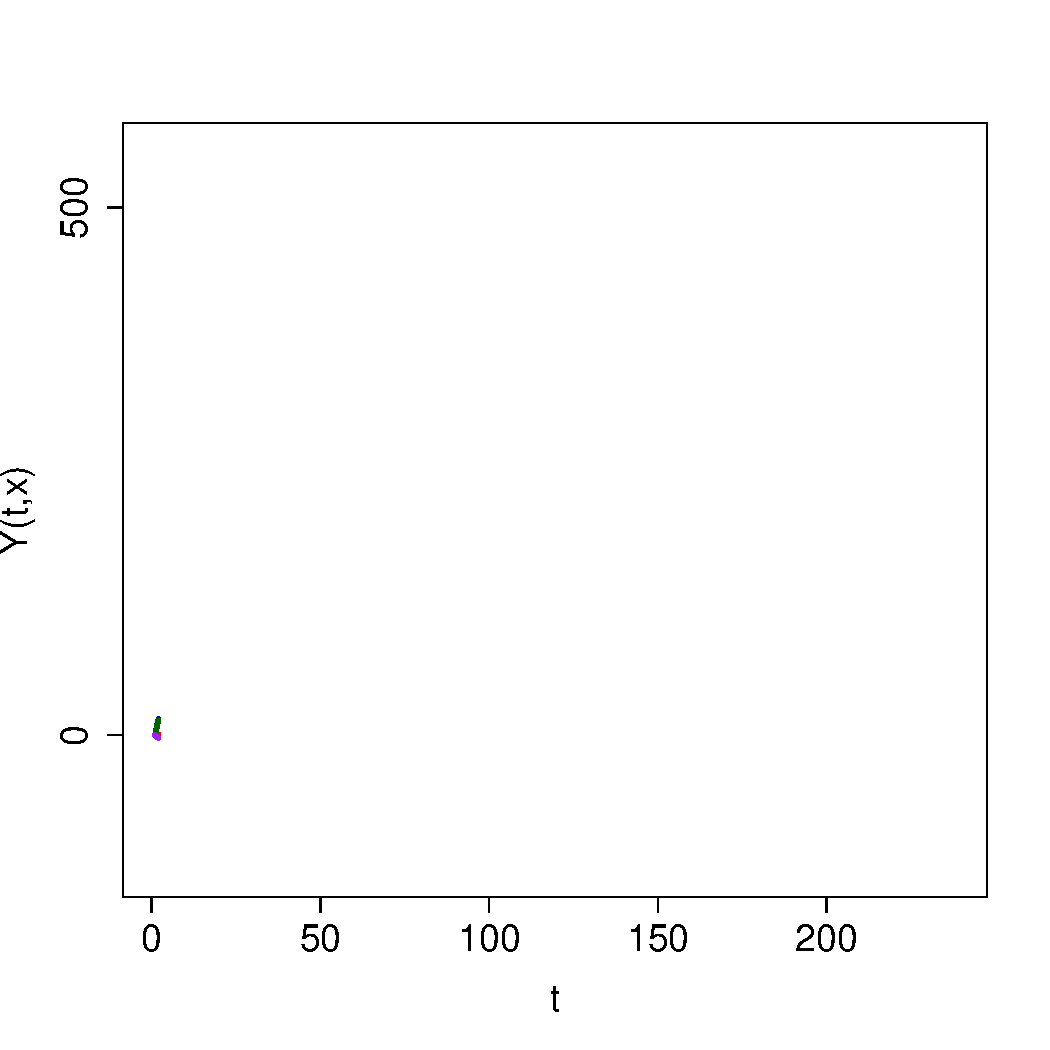
\includegraphics[height=\textheight]{\figdir/biz/AFOSR2013/animation/pdf2/animation_0002.pdf}\end{figure}\end{frame}
\begin{frame}\frametitle{A Typical Ranking \& Selection Procedure}\begin{figure}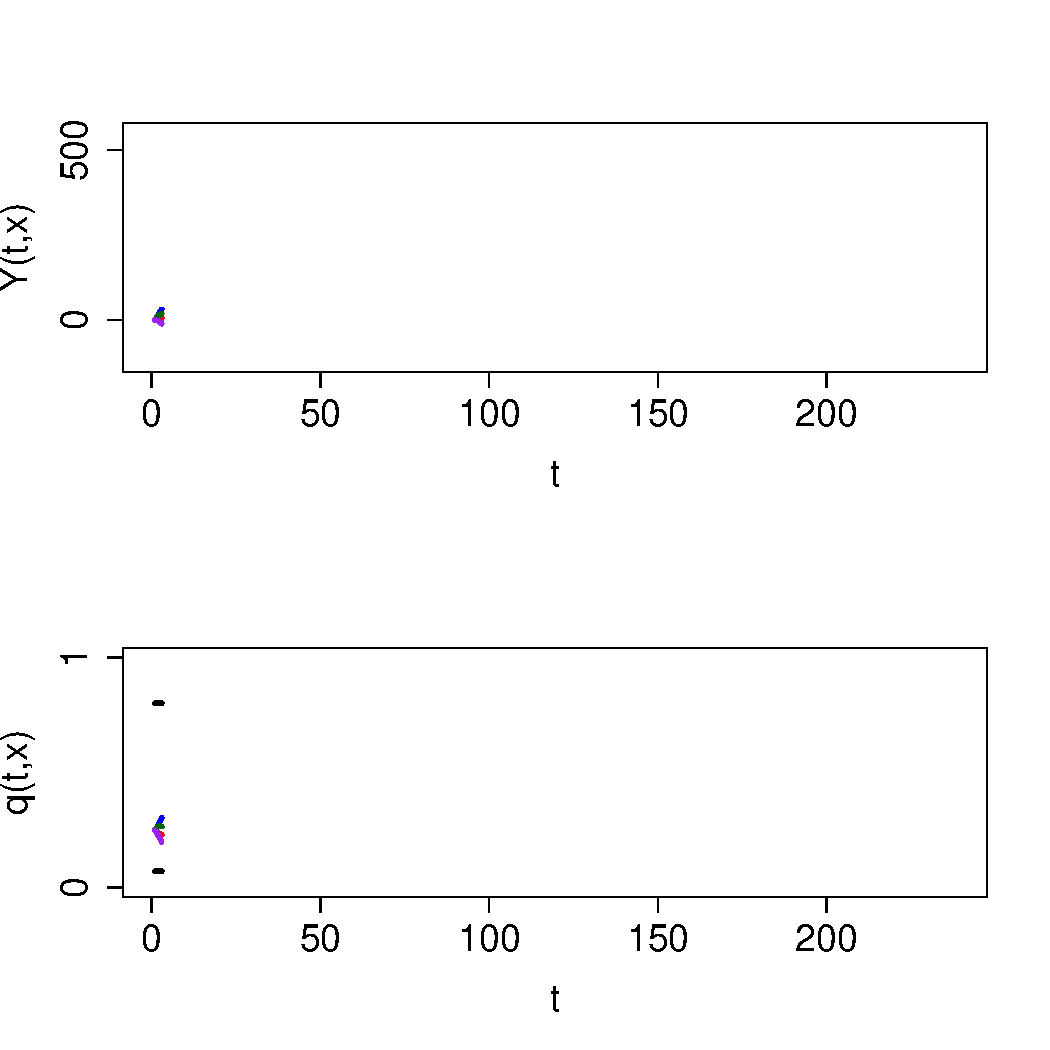
\includegraphics[height=\textheight]{\figdir/biz/AFOSR2013/animation/pdf2/animation_0003.pdf}\end{figure}\end{frame}
\begin{frame}\frametitle{A Typical Ranking \& Selection Procedure}\begin{figure}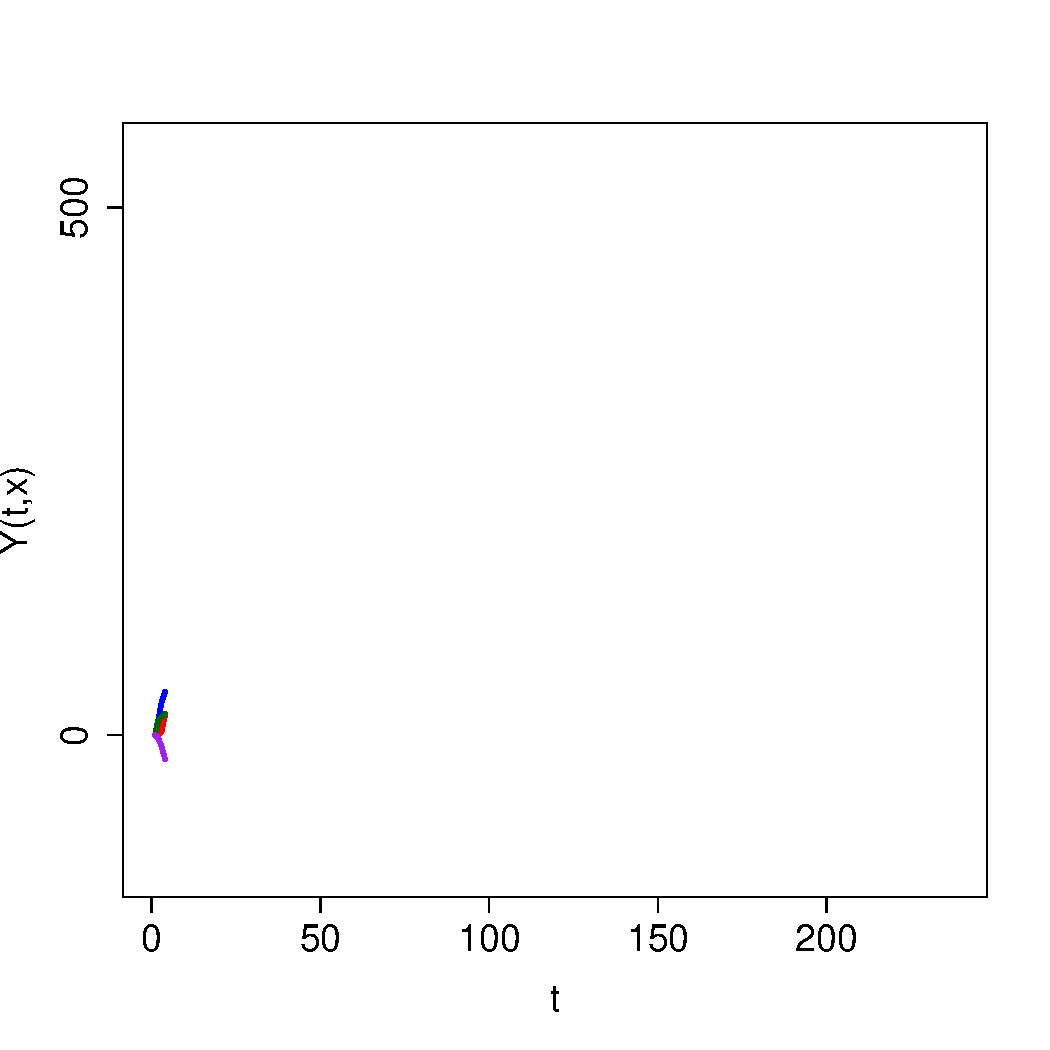
\includegraphics[height=\textheight]{\figdir/biz/AFOSR2013/animation/pdf2/animation_0004.pdf}\end{figure}\end{frame}
\begin{frame}\frametitle{A Typical Ranking \& Selection Procedure}\begin{figure}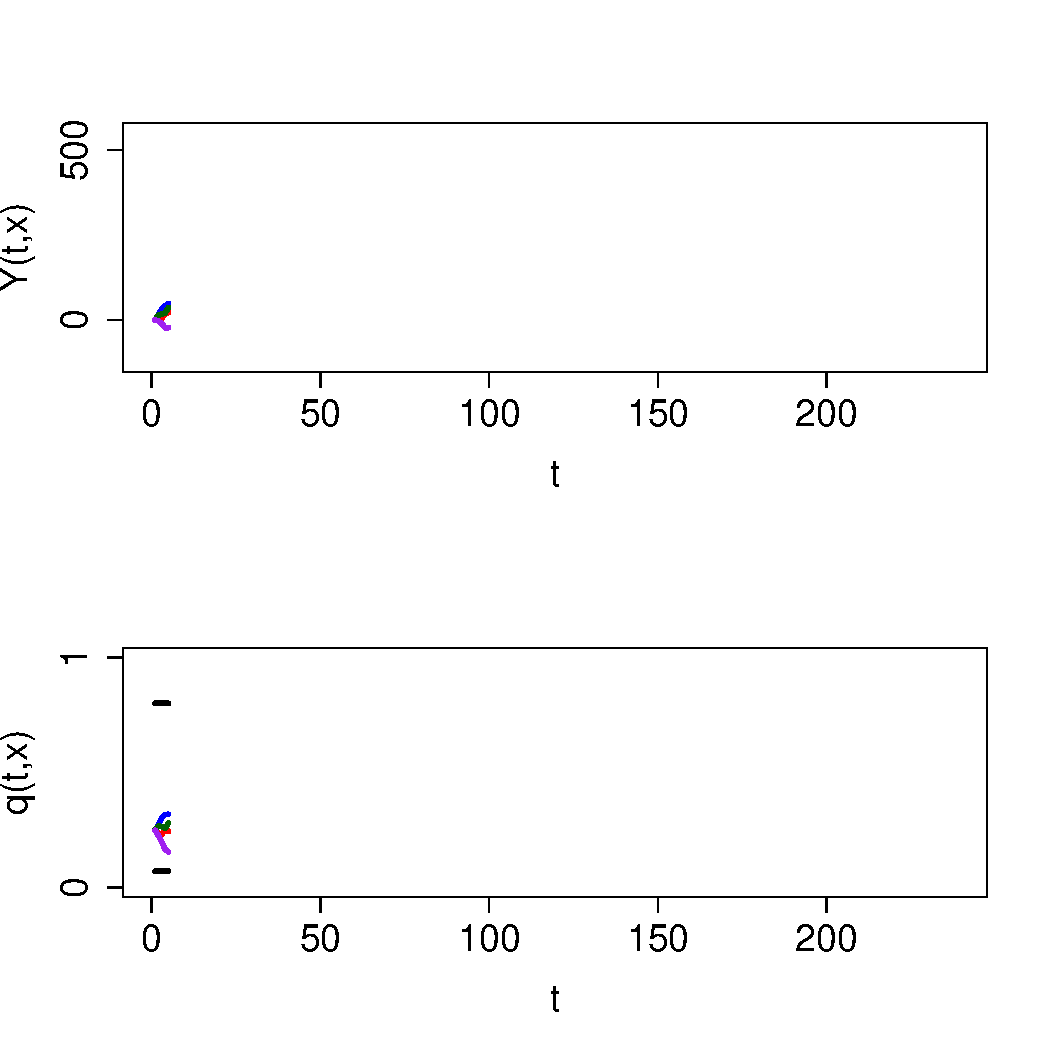
\includegraphics[height=\textheight]{\figdir/biz/AFOSR2013/animation/pdf2/animation_0005.pdf}\end{figure}\end{frame}
\begin{frame}\frametitle{A Typical Ranking \& Selection Procedure}\begin{figure}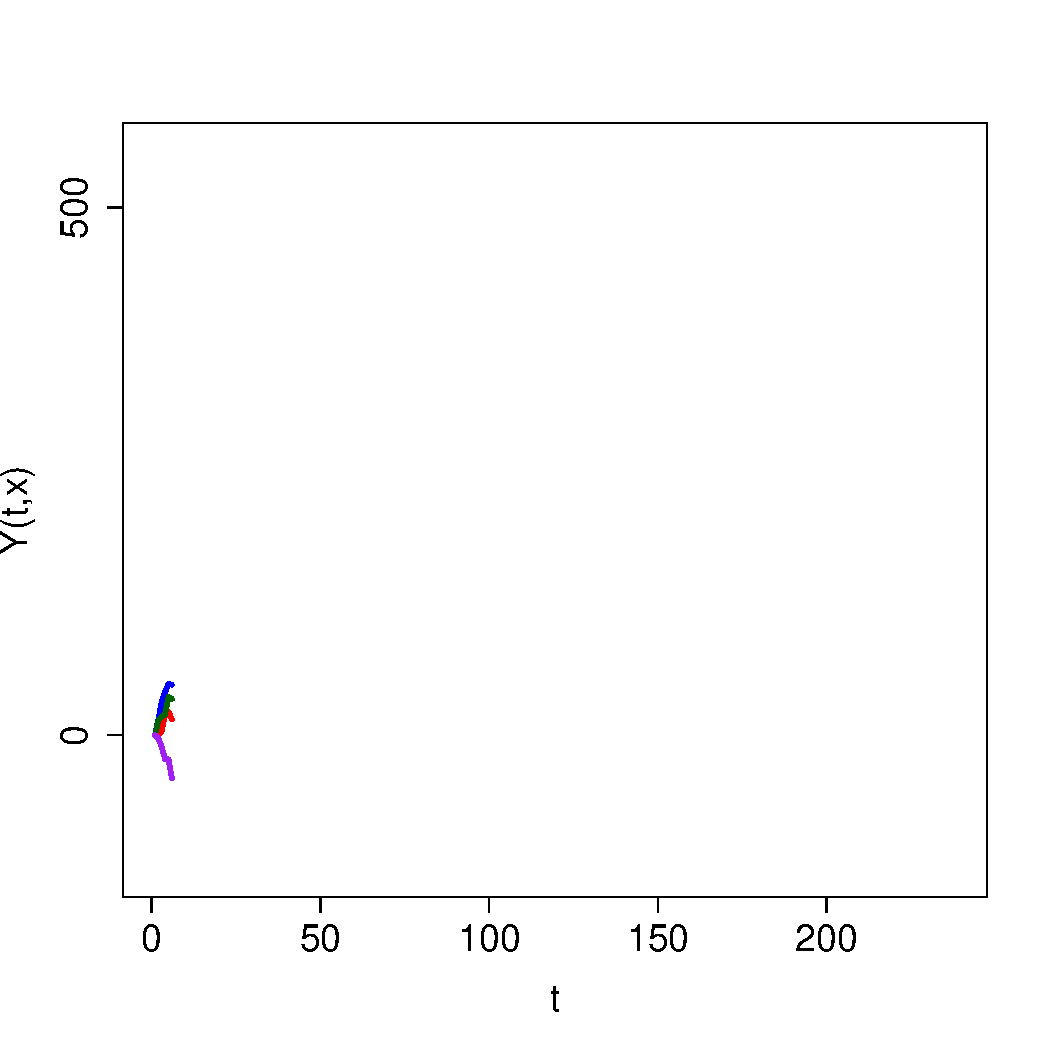
\includegraphics[height=\textheight]{\figdir/biz/AFOSR2013/animation/pdf2/animation_0006.pdf}\end{figure}\end{frame}
\begin{frame}\frametitle{A Typical Ranking \& Selection Procedure}\begin{figure}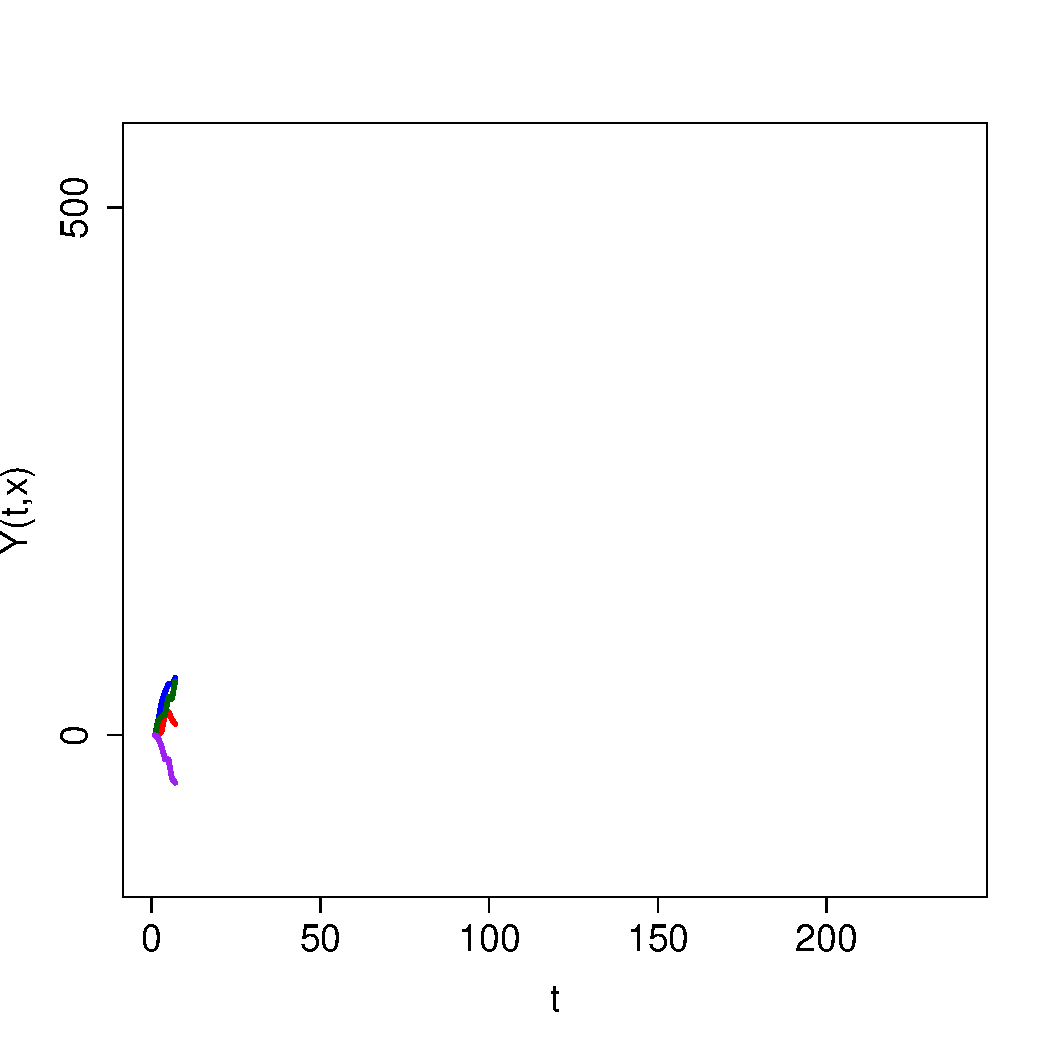
\includegraphics[height=\textheight]{\figdir/biz/AFOSR2013/animation/pdf2/animation_0007.pdf}\end{figure}\end{frame}
\begin{frame}\frametitle{A Typical Ranking \& Selection Procedure}\begin{figure}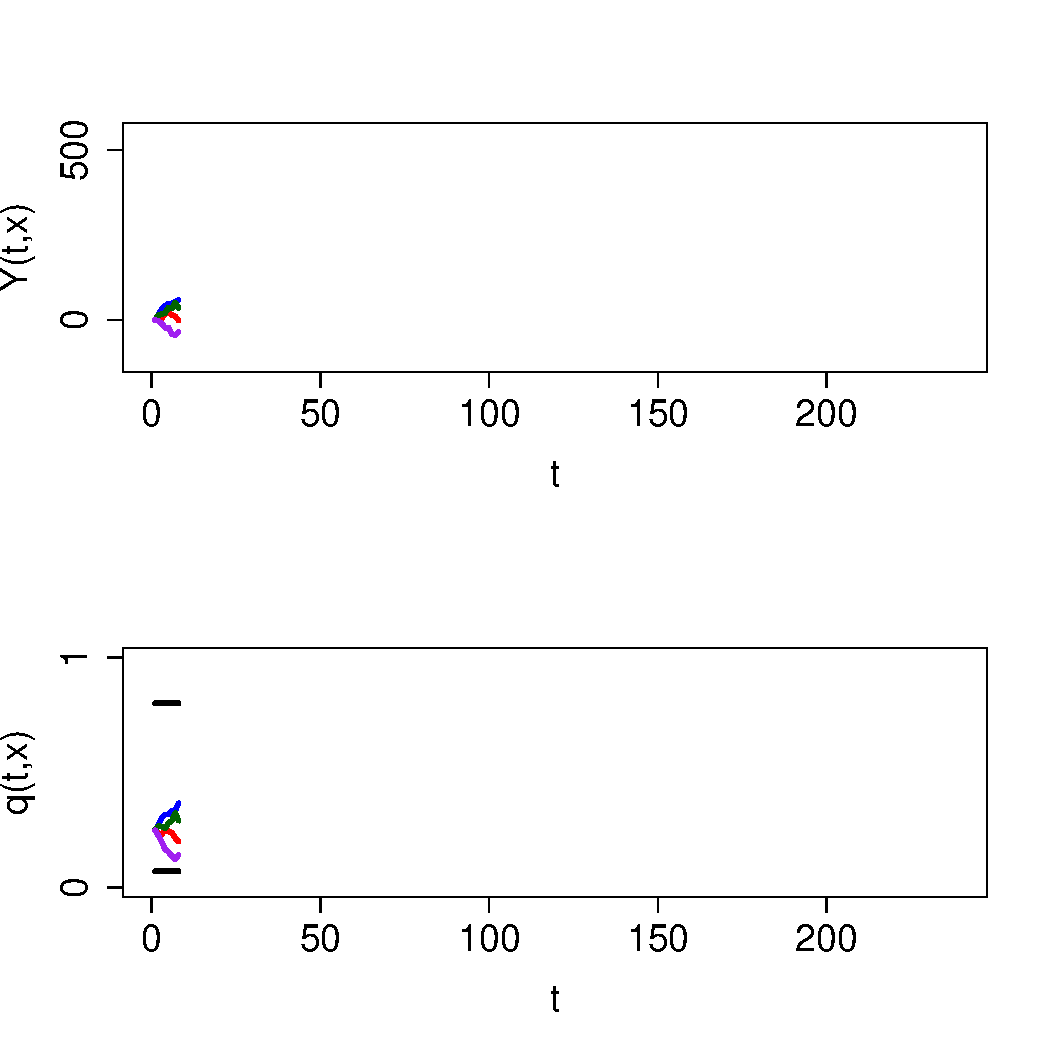
\includegraphics[height=\textheight]{\figdir/biz/AFOSR2013/animation/pdf2/animation_0008.pdf}\end{figure}\end{frame}
\begin{frame}\frametitle{A Typical Ranking \& Selection Procedure}\begin{figure}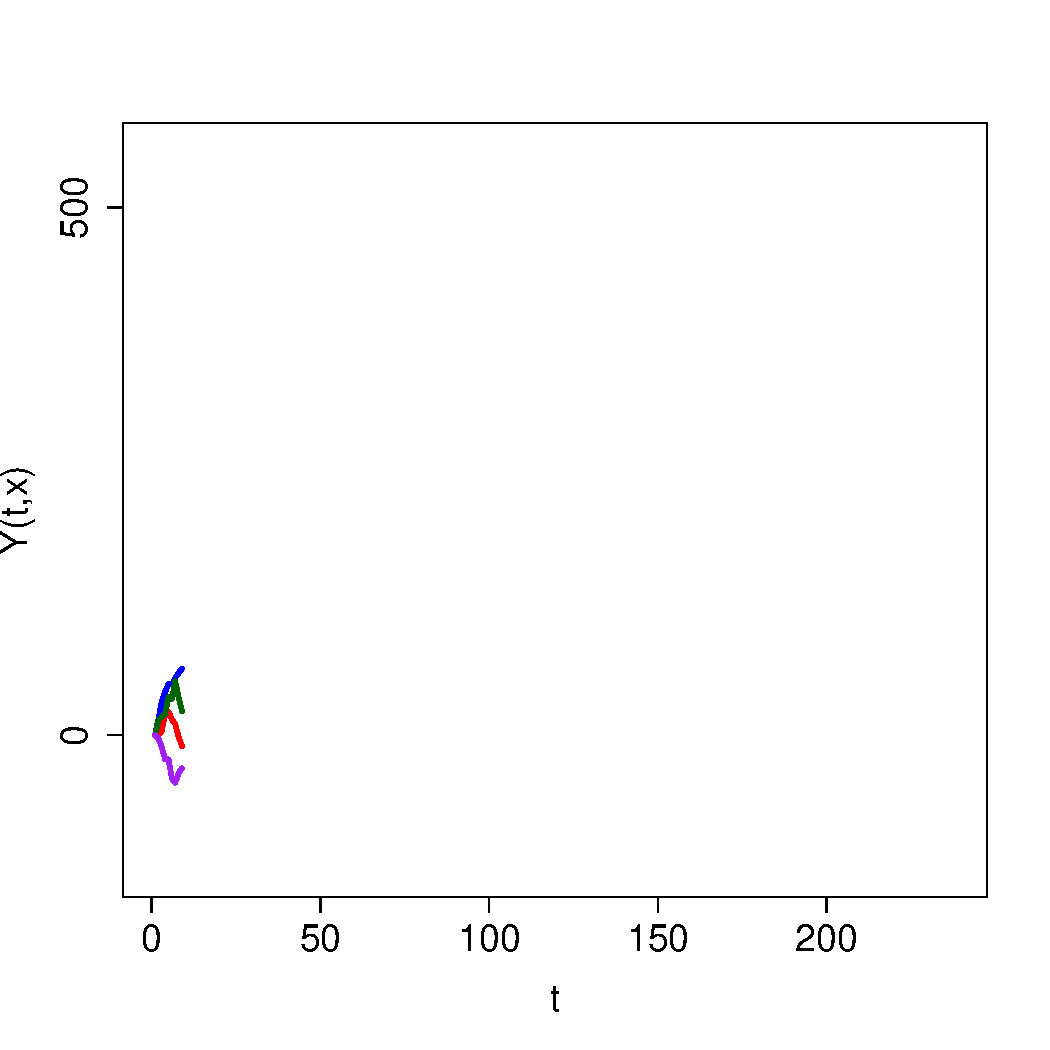
\includegraphics[height=\textheight]{\figdir/biz/AFOSR2013/animation/pdf2/animation_0009.pdf}\end{figure}\end{frame}
\begin{frame}\frametitle{A Typical Ranking \& Selection Procedure}\begin{figure}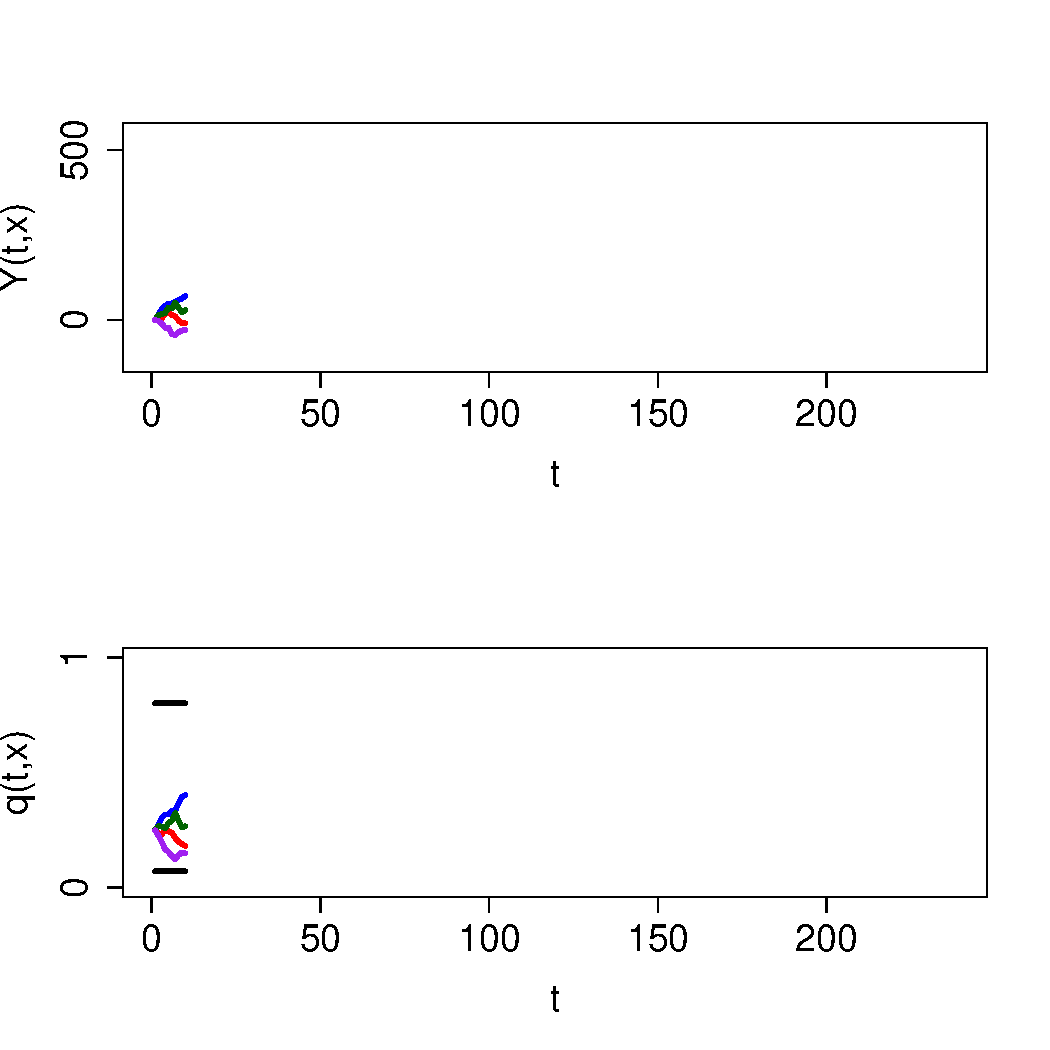
\includegraphics[height=\textheight]{\figdir/biz/AFOSR2013/animation/pdf2/animation_0010.pdf}\end{figure}\end{frame}
\begin{frame}\frametitle{A Typical Ranking \& Selection Procedure}\begin{figure}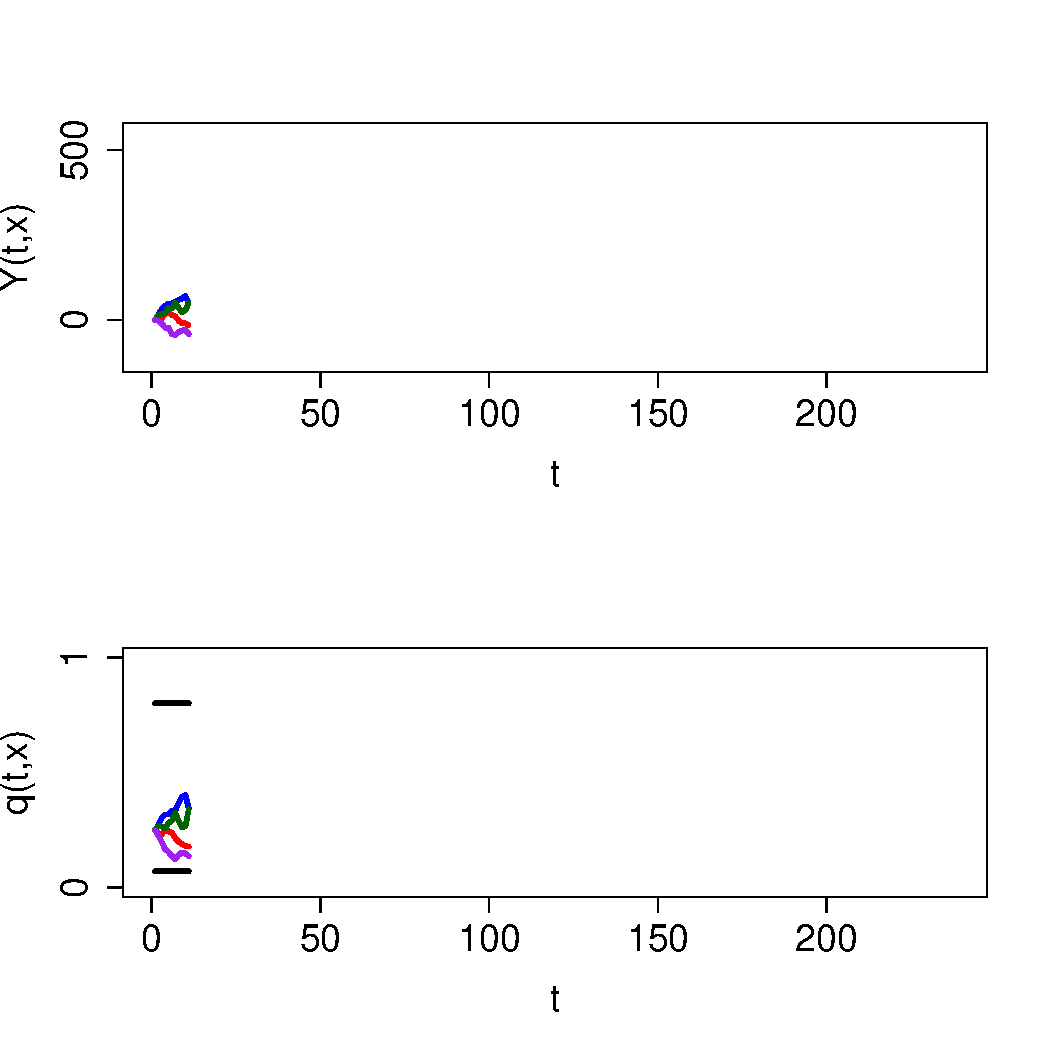
\includegraphics[height=\textheight]{\figdir/biz/AFOSR2013/animation/pdf2/animation_0011.pdf}\end{figure}\end{frame}
\begin{frame}\frametitle{A Typical Ranking \& Selection Procedure}\begin{figure}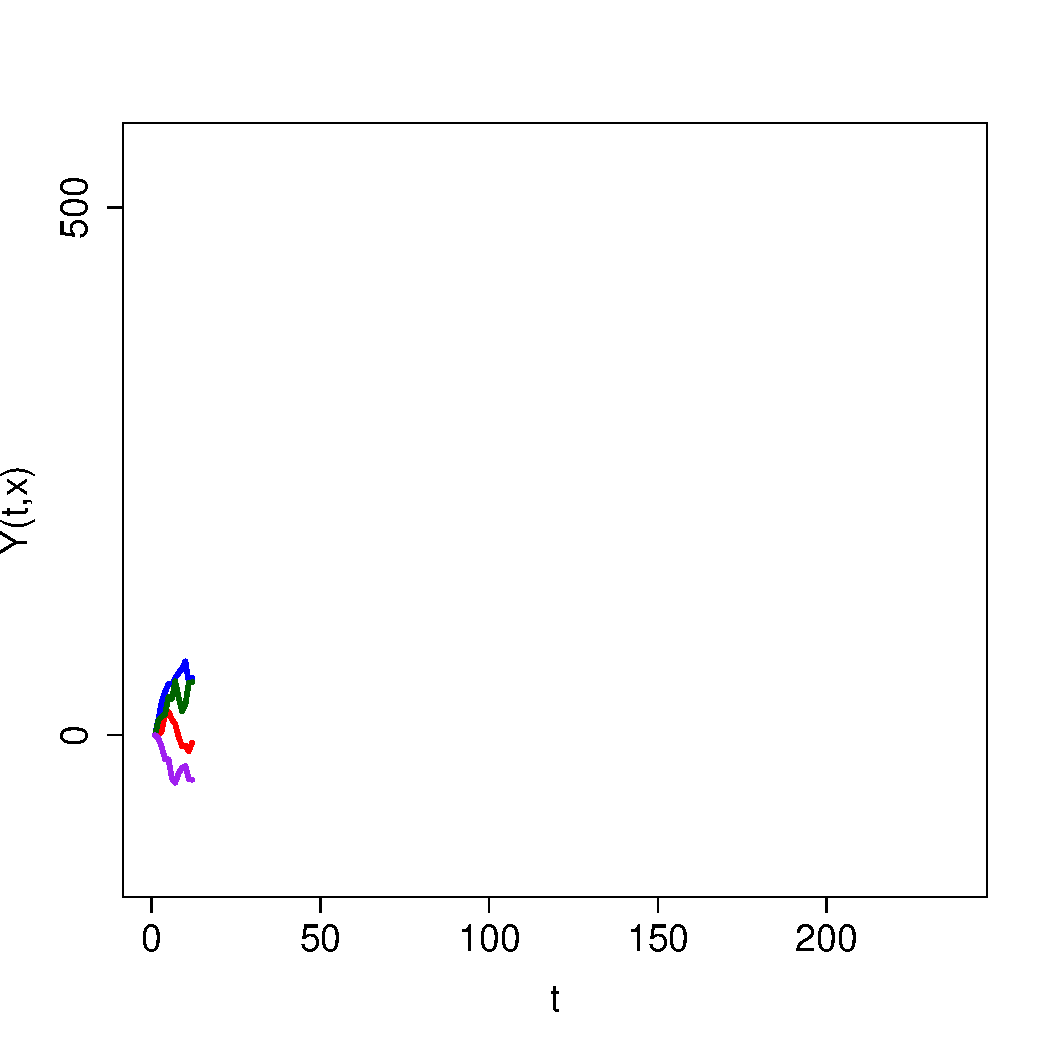
\includegraphics[height=\textheight]{\figdir/biz/AFOSR2013/animation/pdf2/animation_0012.pdf}\end{figure}\end{frame}
\begin{frame}\frametitle{A Typical Ranking \& Selection Procedure}\begin{figure}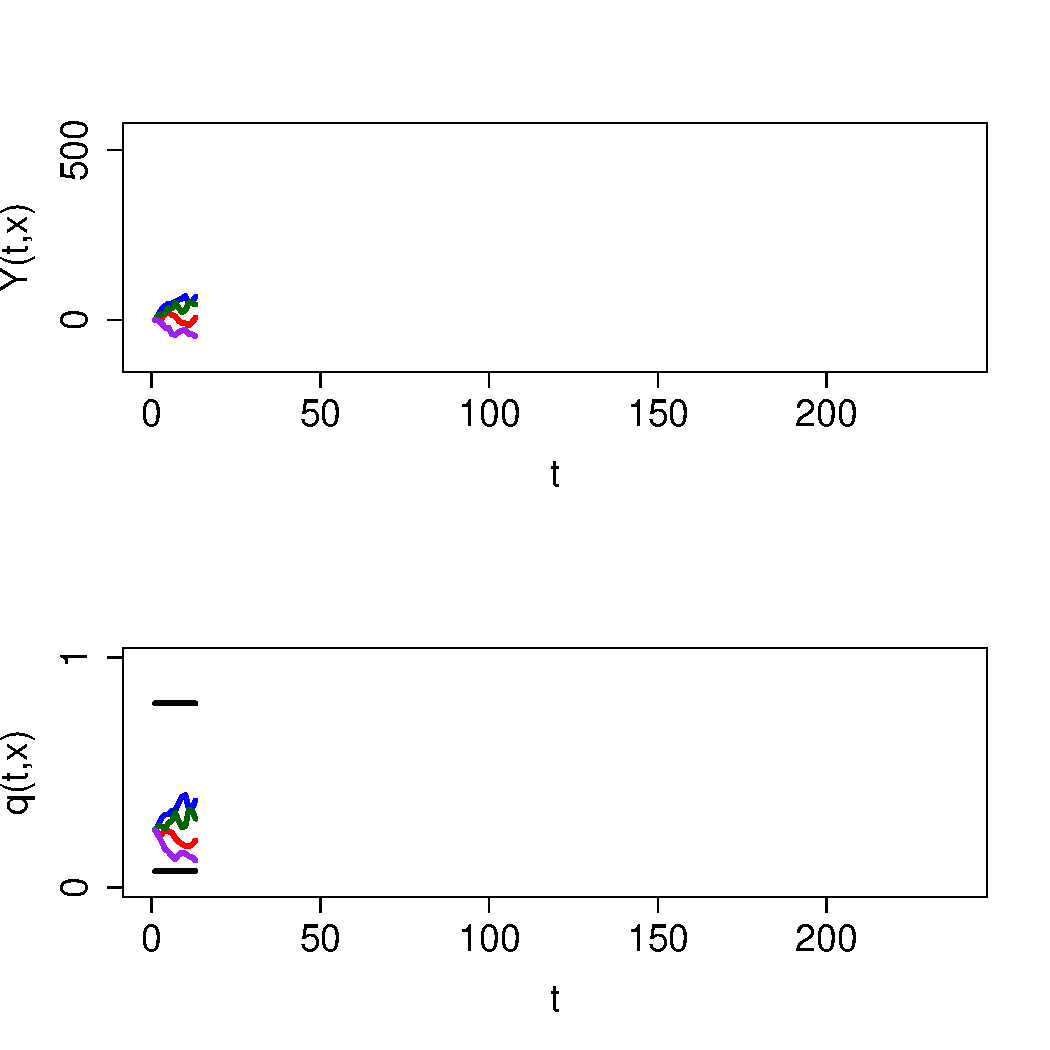
\includegraphics[height=\textheight]{\figdir/biz/AFOSR2013/animation/pdf2/animation_0013.pdf}\end{figure}\end{frame}
\begin{frame}\frametitle{A Typical Ranking \& Selection Procedure}\begin{figure}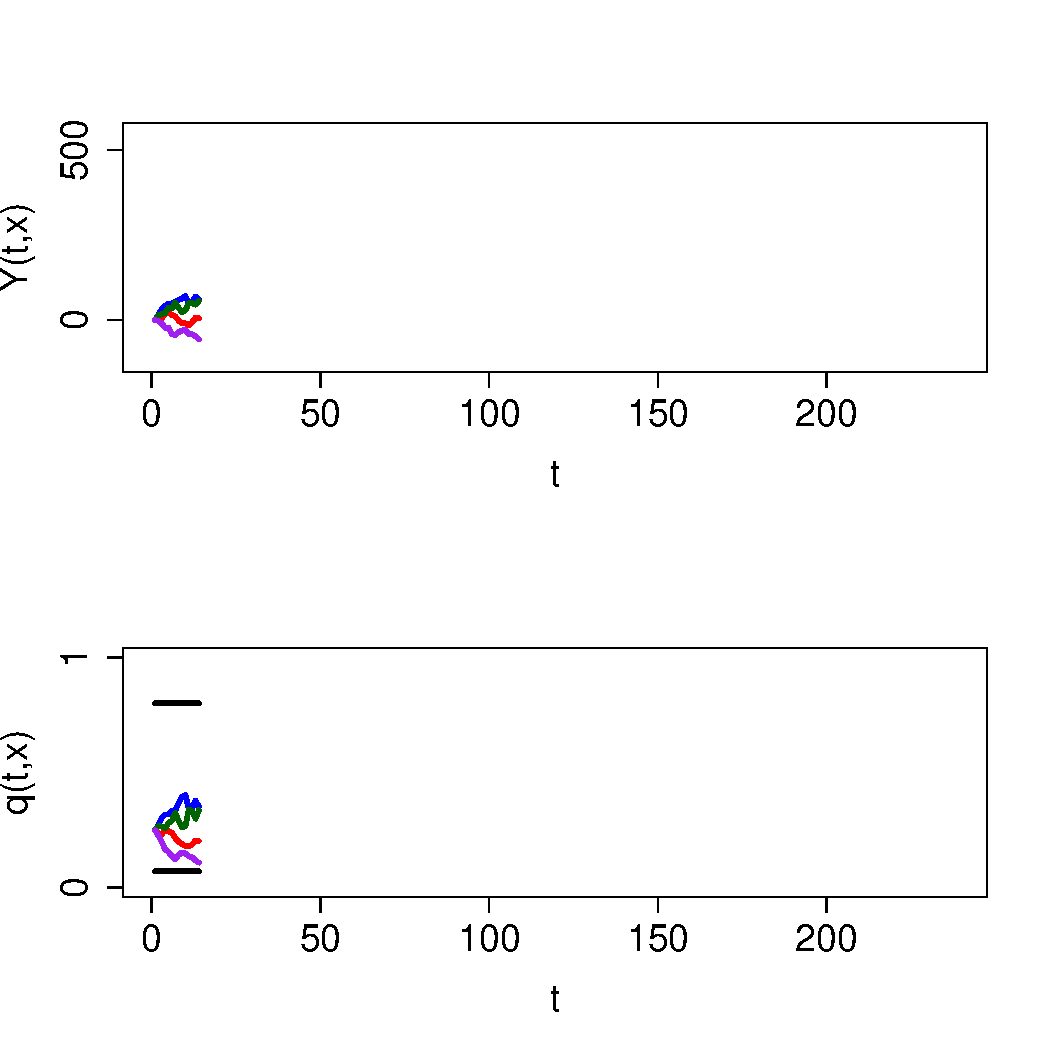
\includegraphics[height=\textheight]{\figdir/biz/AFOSR2013/animation/pdf2/animation_0014.pdf}\end{figure}\end{frame}
\begin{frame}\frametitle{A Typical Ranking \& Selection Procedure}\begin{figure}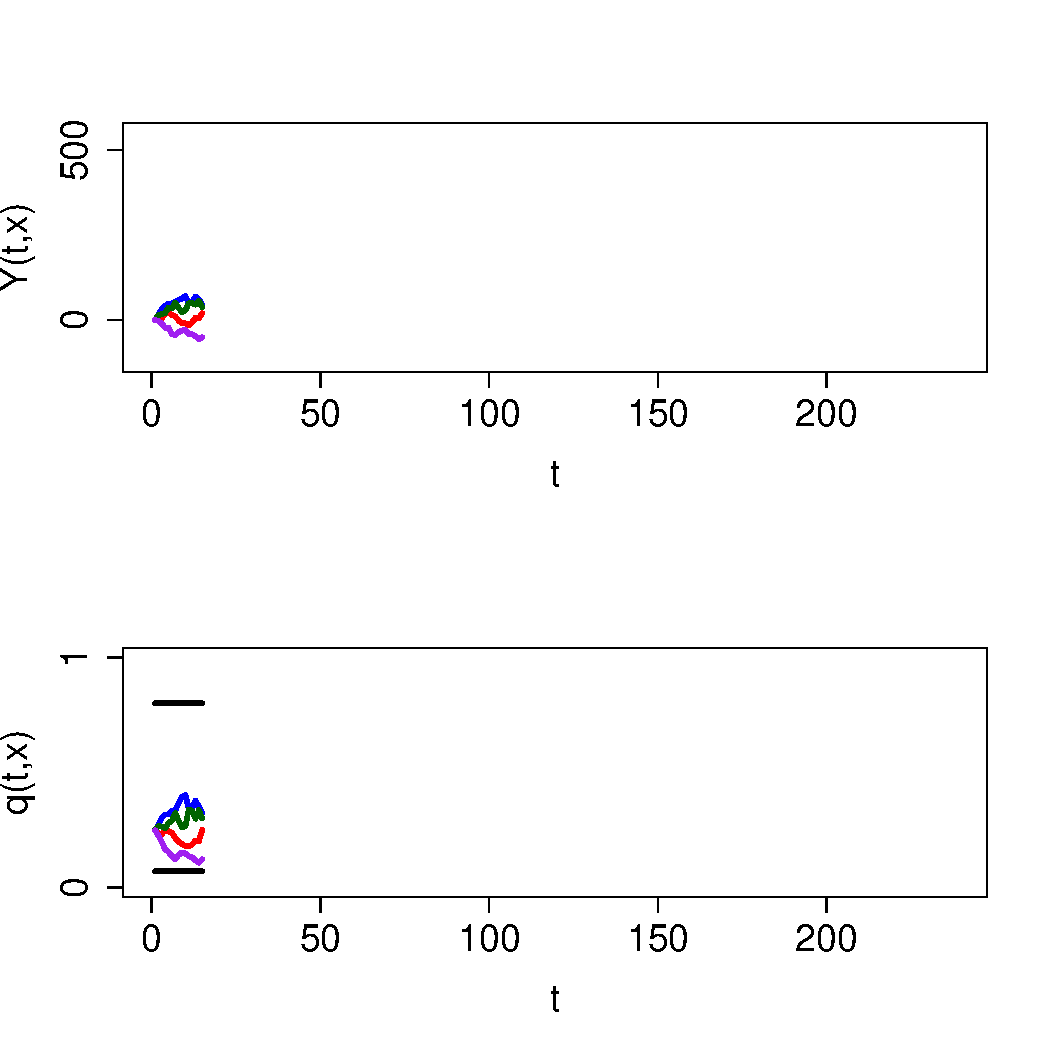
\includegraphics[height=\textheight]{\figdir/biz/AFOSR2013/animation/pdf2/animation_0015.pdf}\end{figure}\end{frame}
\begin{frame}\frametitle{A Typical Ranking \& Selection Procedure}\begin{figure}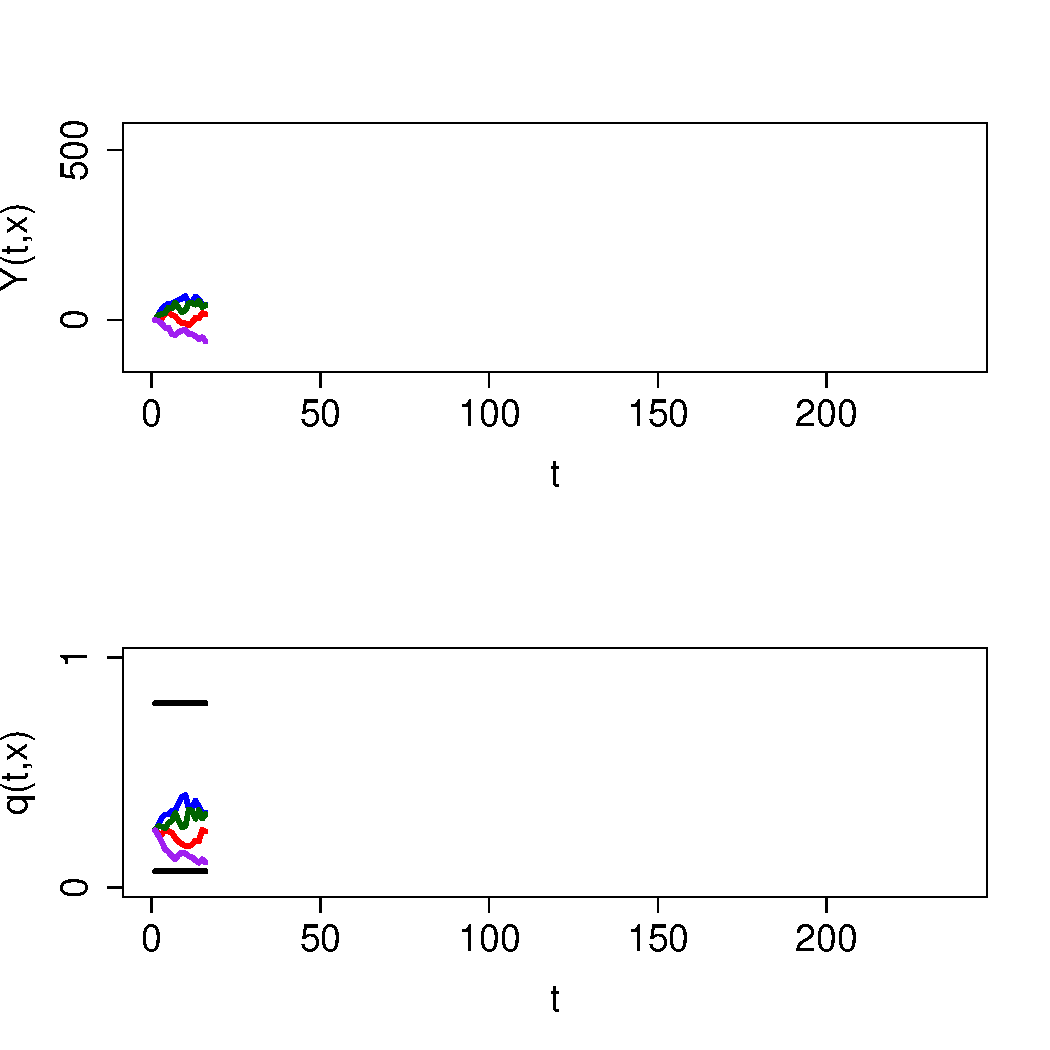
\includegraphics[height=\textheight]{\figdir/biz/AFOSR2013/animation/pdf2/animation_0016.pdf}\end{figure}\end{frame}
\begin{frame}\frametitle{A Typical Ranking \& Selection Procedure}\begin{figure}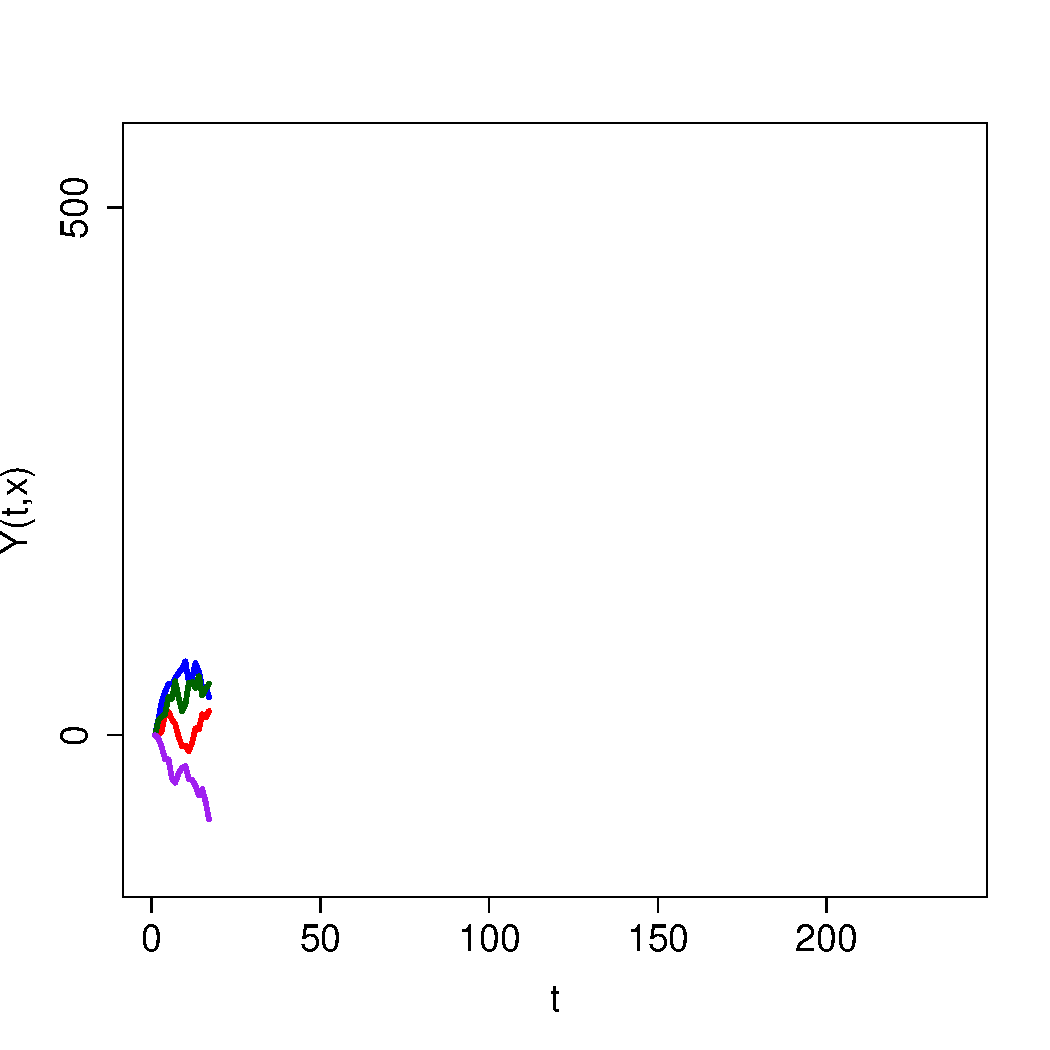
\includegraphics[height=\textheight]{\figdir/biz/AFOSR2013/animation/pdf2/animation_0017.pdf}\end{figure}\end{frame}
\begin{frame}\frametitle{A Typical Ranking \& Selection Procedure}\begin{figure}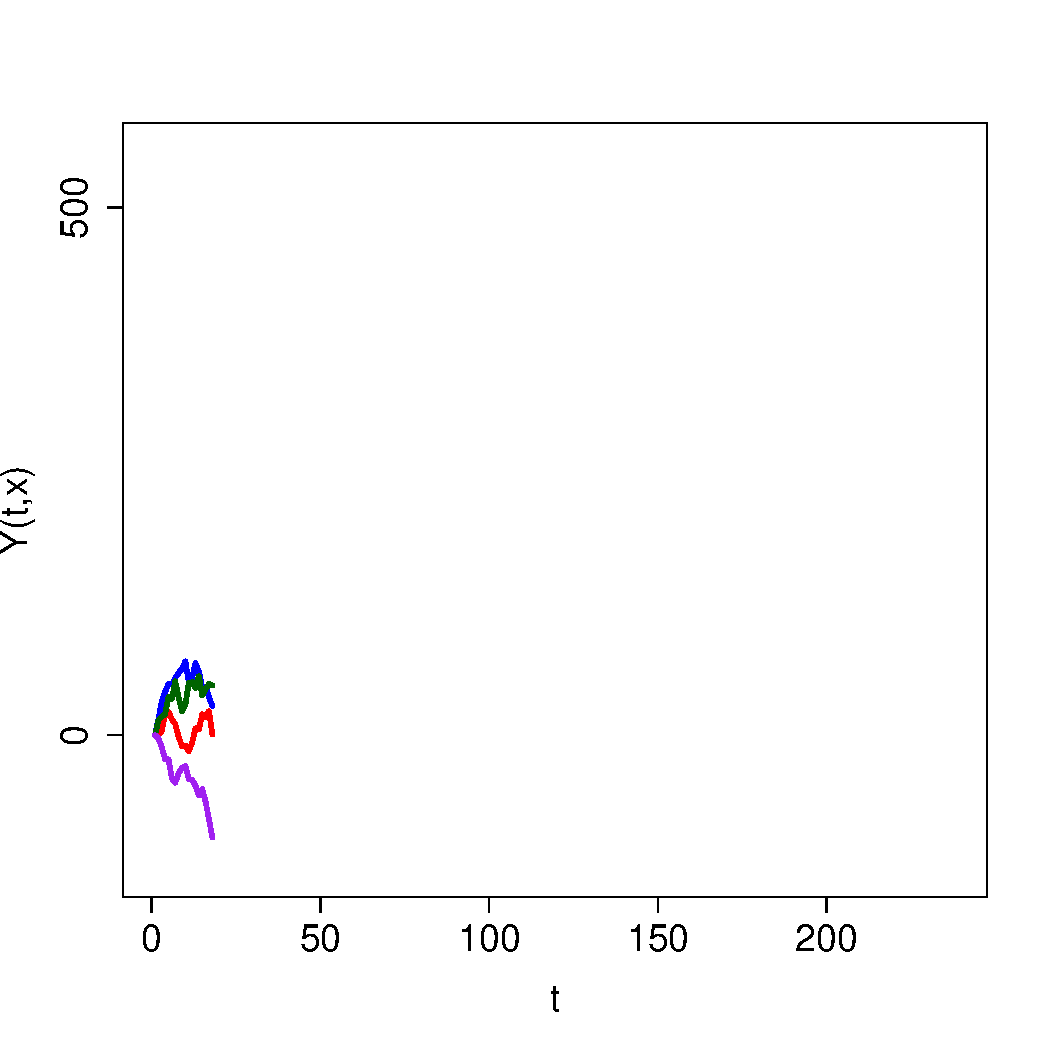
\includegraphics[height=\textheight]{\figdir/biz/AFOSR2013/animation/pdf2/animation_0018.pdf}\end{figure}\end{frame}
\begin{frame}\frametitle{A Typical Ranking \& Selection Procedure}\begin{figure}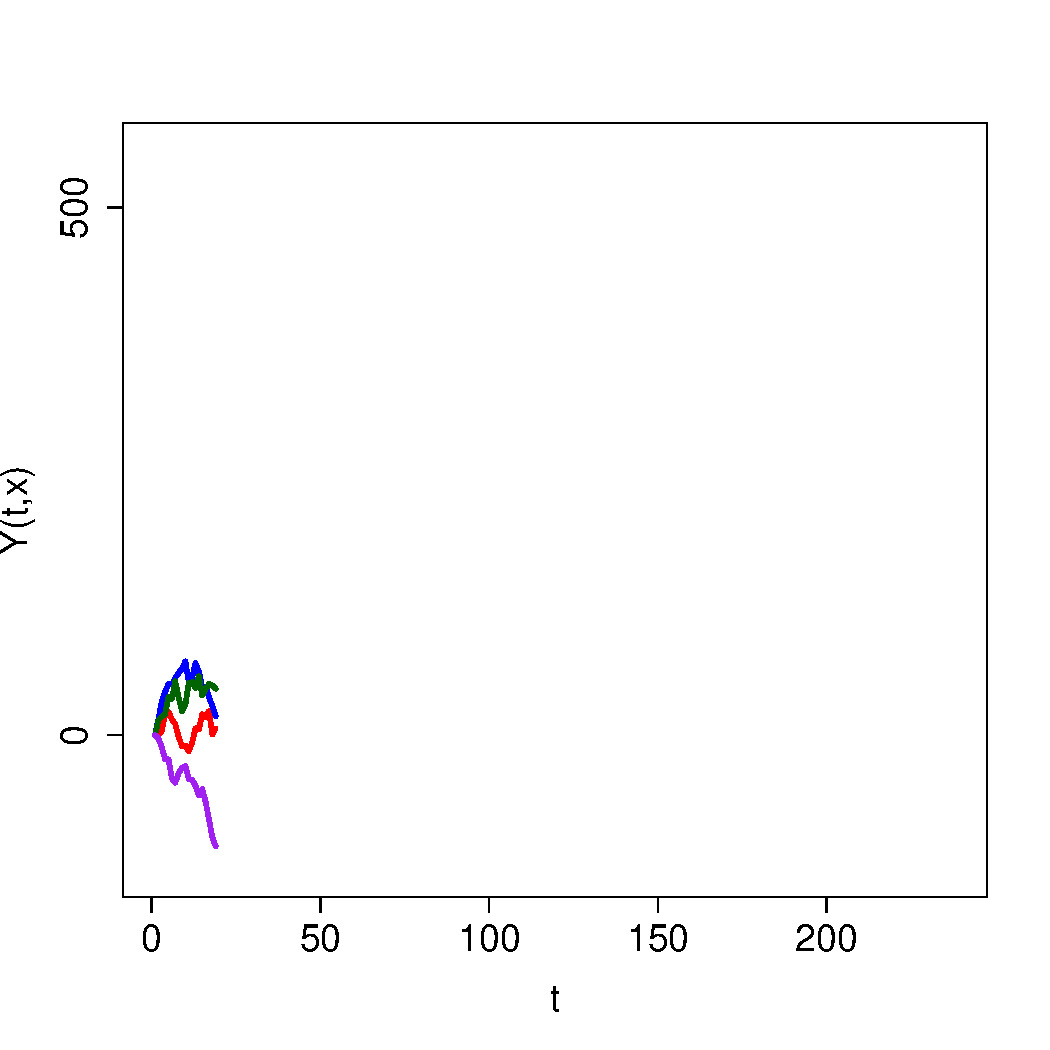
\includegraphics[height=\textheight]{\figdir/biz/AFOSR2013/animation/pdf2/animation_0019.pdf}\end{figure}\end{frame}
\begin{frame}\frametitle{A Typical Ranking \& Selection Procedure}\begin{figure}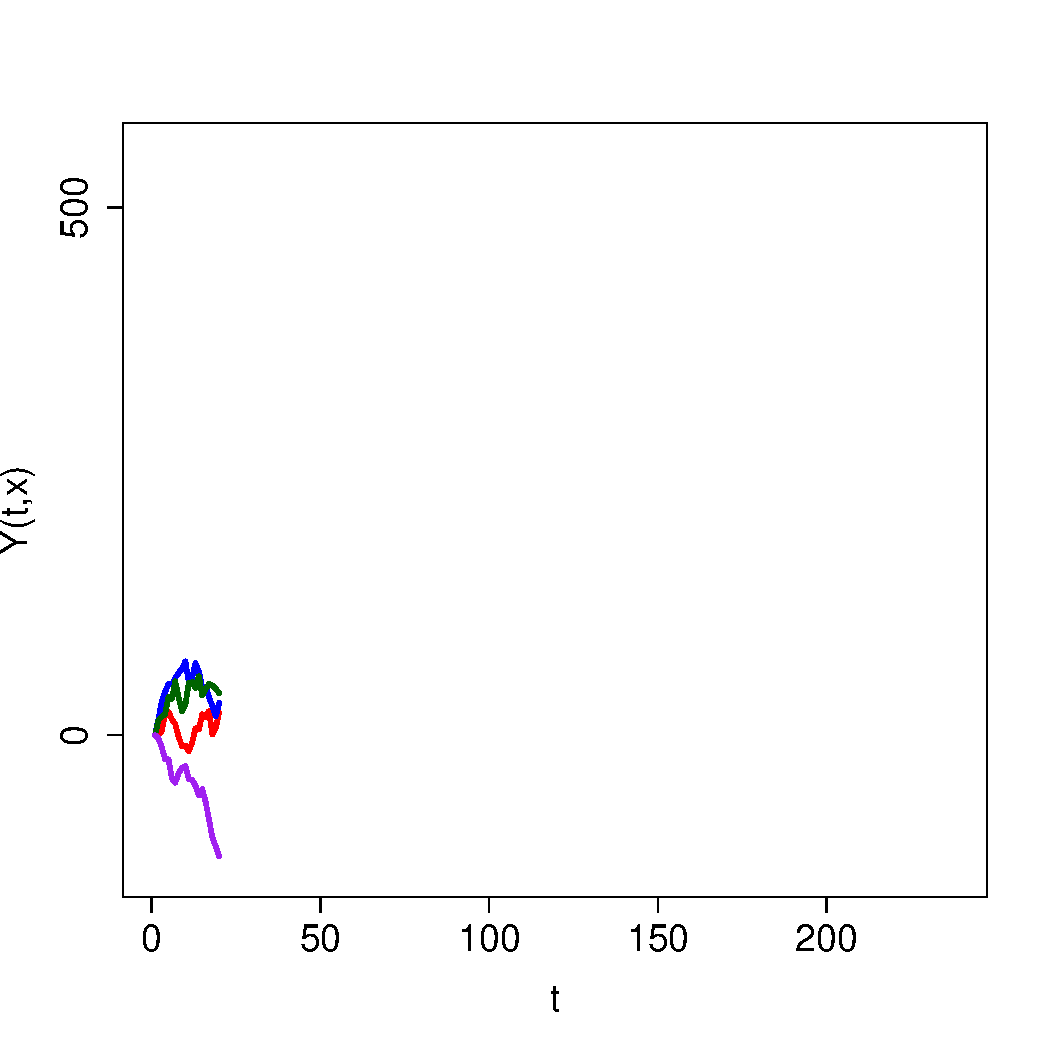
\includegraphics[height=\textheight]{\figdir/biz/AFOSR2013/animation/pdf2/animation_0020.pdf}\end{figure}\end{frame}
\begin{frame}\frametitle{A Typical Ranking \& Selection Procedure}\begin{figure}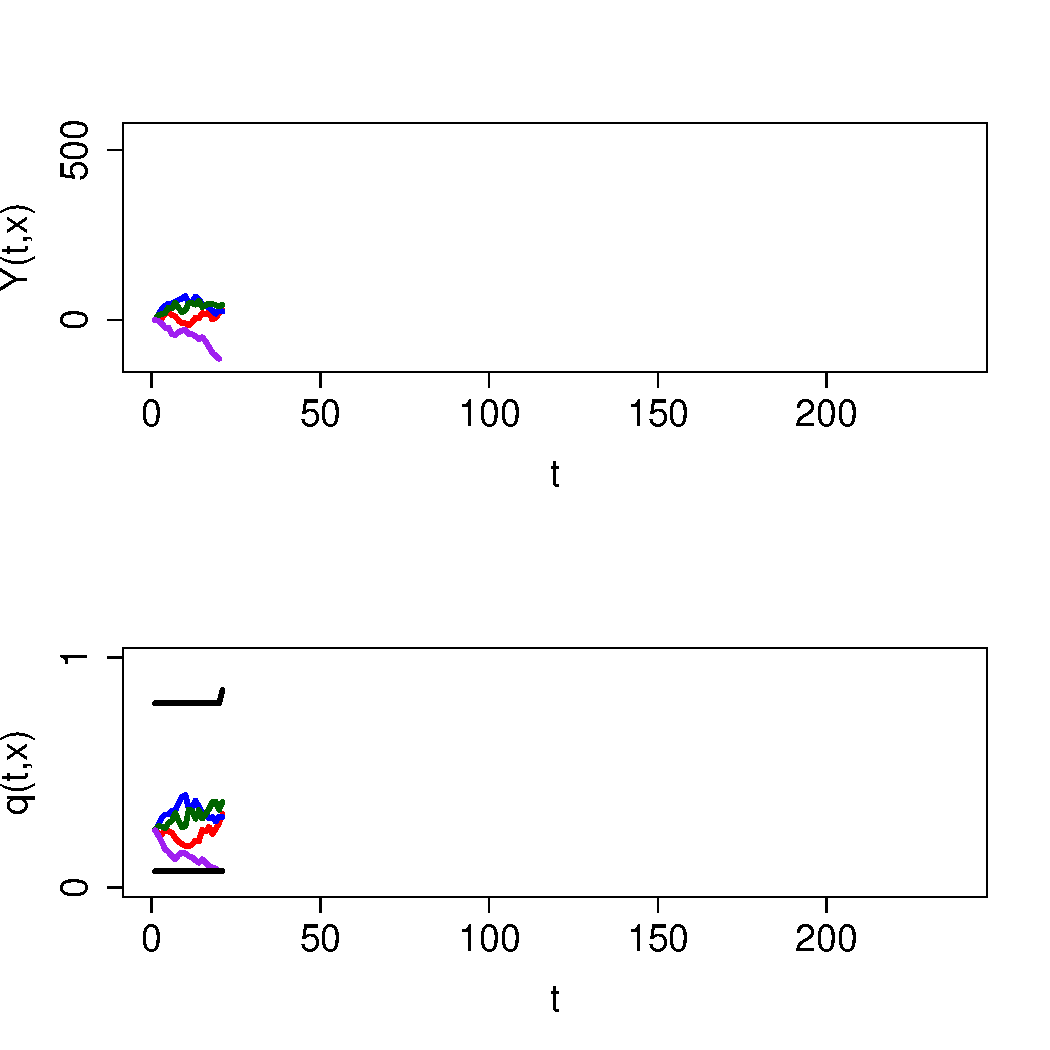
\includegraphics[height=\textheight]{\figdir/biz/AFOSR2013/animation/pdf2/animation_0021.pdf}\end{figure}\end{frame}
\begin{frame}\frametitle{A Typical Ranking \& Selection Procedure}\begin{figure}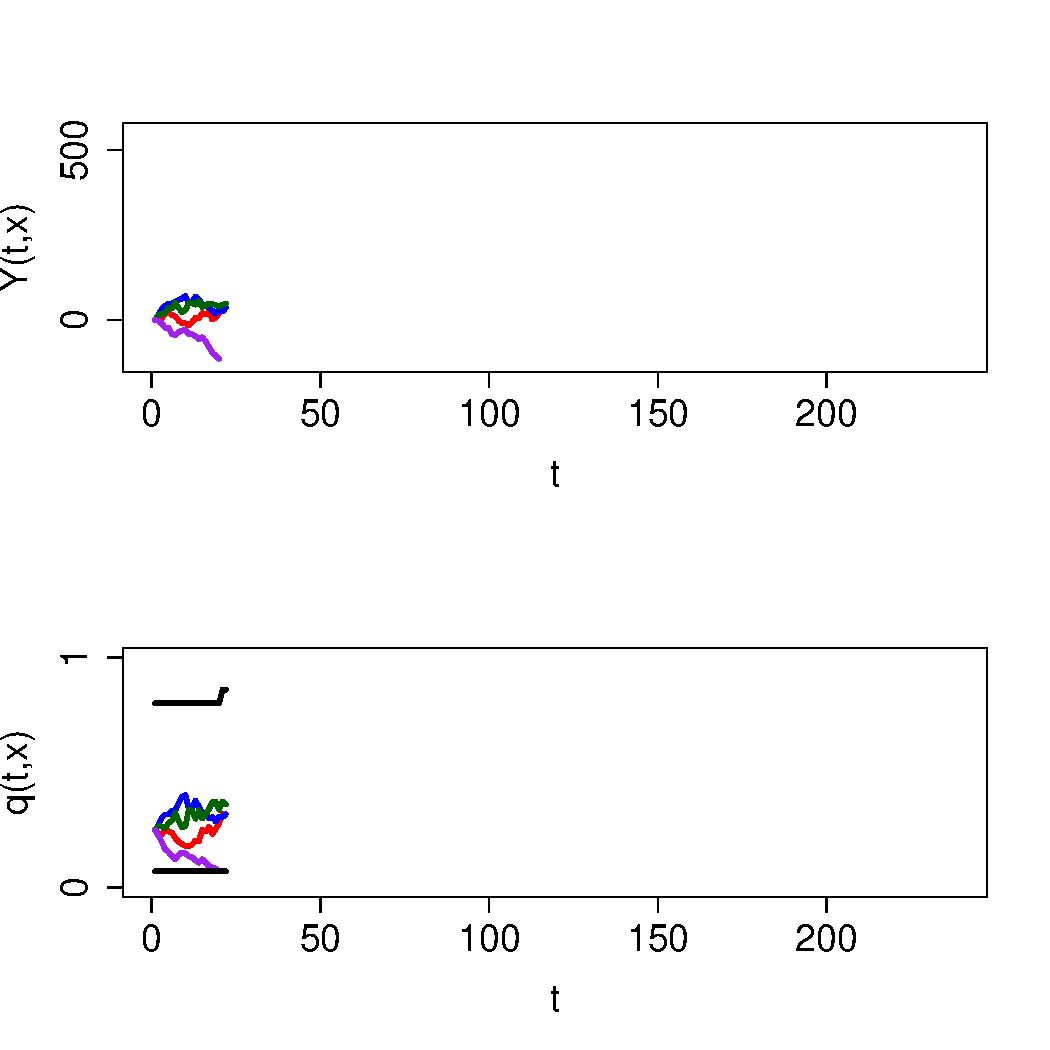
\includegraphics[height=\textheight]{\figdir/biz/AFOSR2013/animation/pdf2/animation_0022.pdf}\end{figure}\end{frame}
\begin{frame}\frametitle{A Typical Ranking \& Selection Procedure}\begin{figure}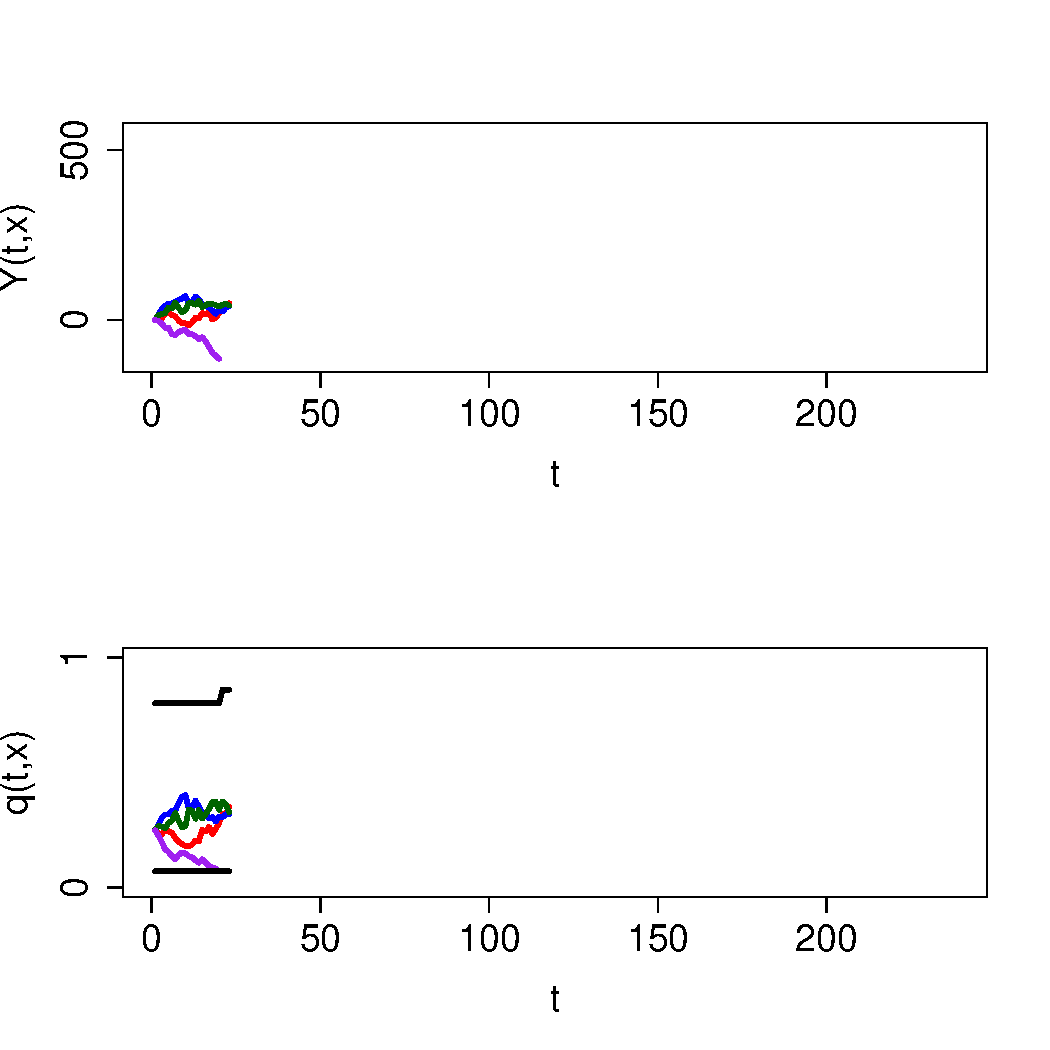
\includegraphics[height=\textheight]{\figdir/biz/AFOSR2013/animation/pdf2/animation_0023.pdf}\end{figure}\end{frame}
\begin{frame}\frametitle{A Typical Ranking \& Selection Procedure}\begin{figure}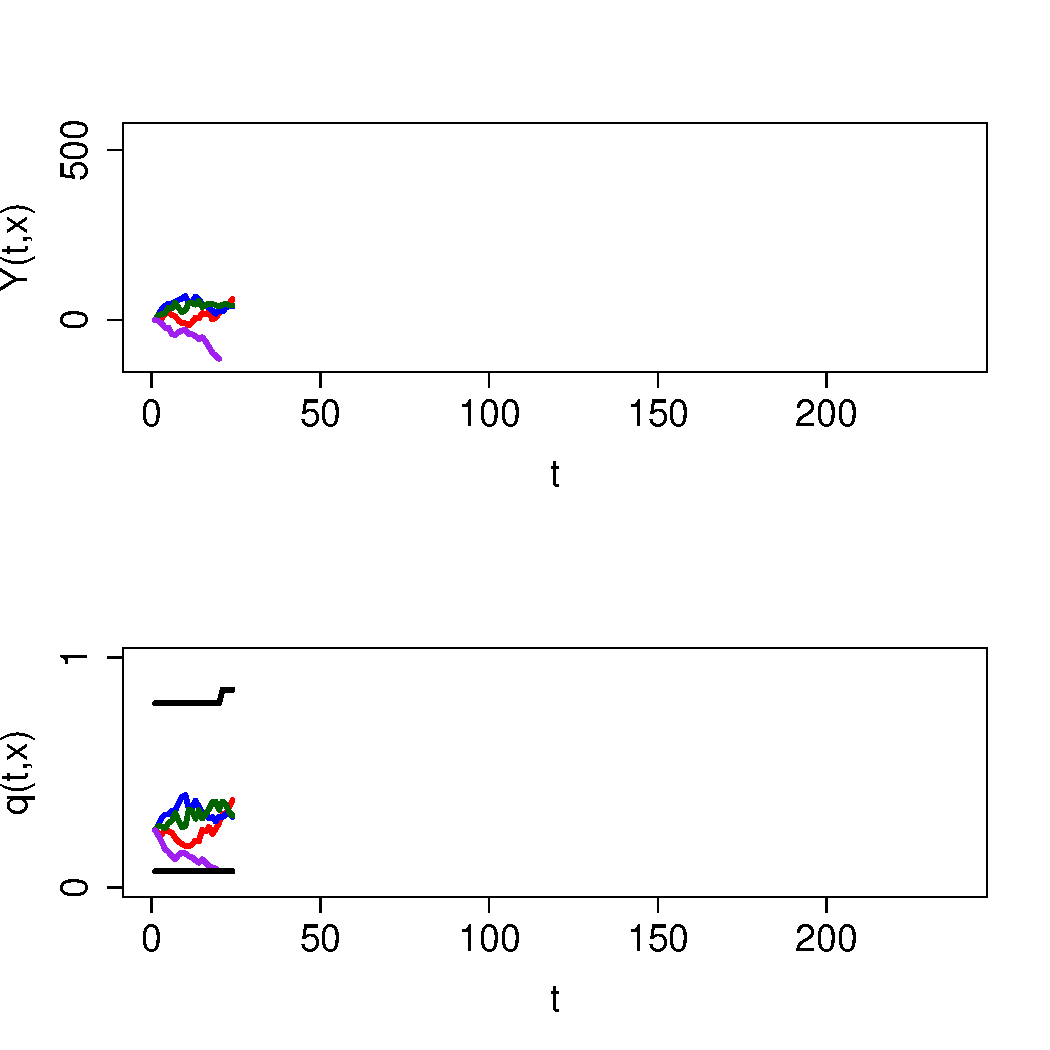
\includegraphics[height=\textheight]{\figdir/biz/AFOSR2013/animation/pdf2/animation_0024.pdf}\end{figure}\end{frame}
\begin{frame}\frametitle{A Typical Ranking \& Selection Procedure}\begin{figure}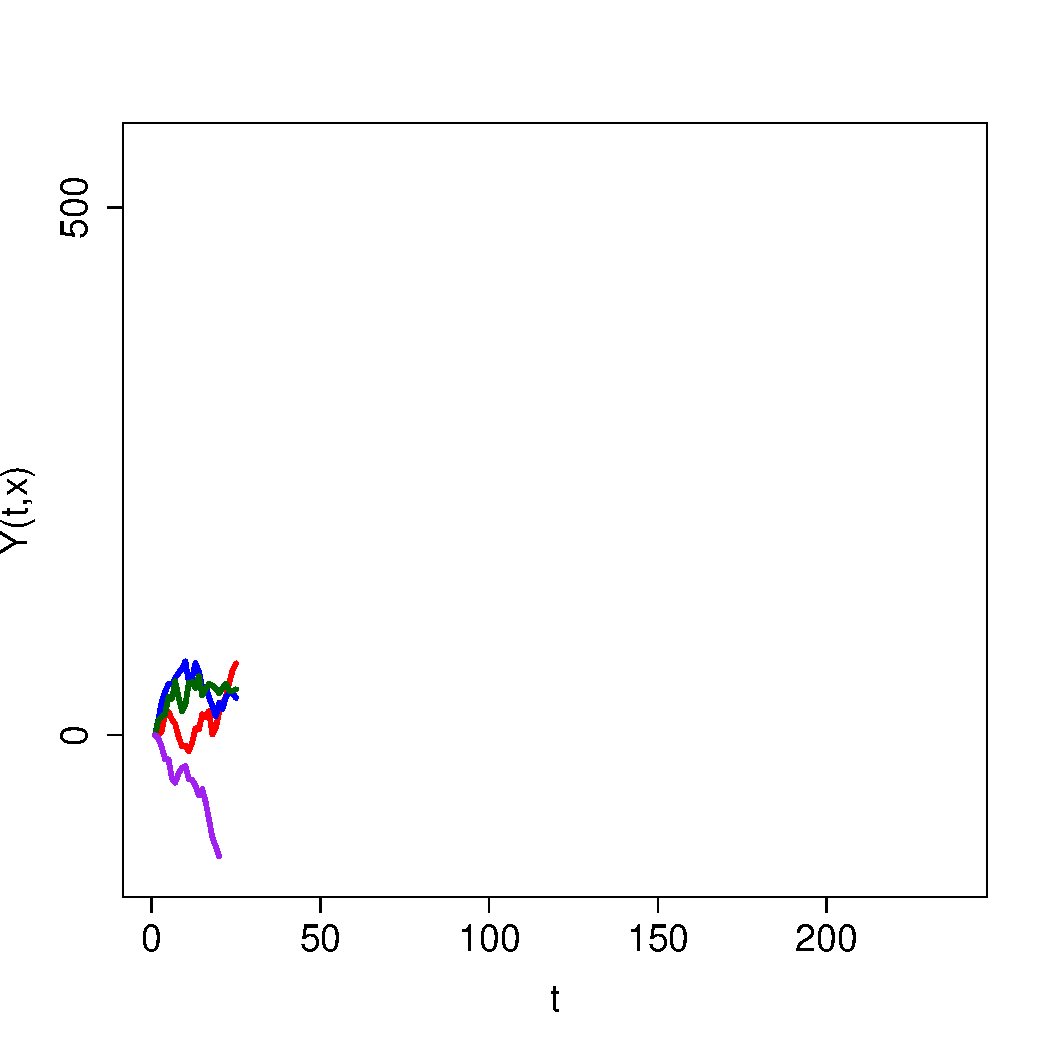
\includegraphics[height=\textheight]{\figdir/biz/AFOSR2013/animation/pdf2/animation_0025.pdf}\end{figure}\end{frame}
\begin{frame}\frametitle{A Typical Ranking \& Selection Procedure}\begin{figure}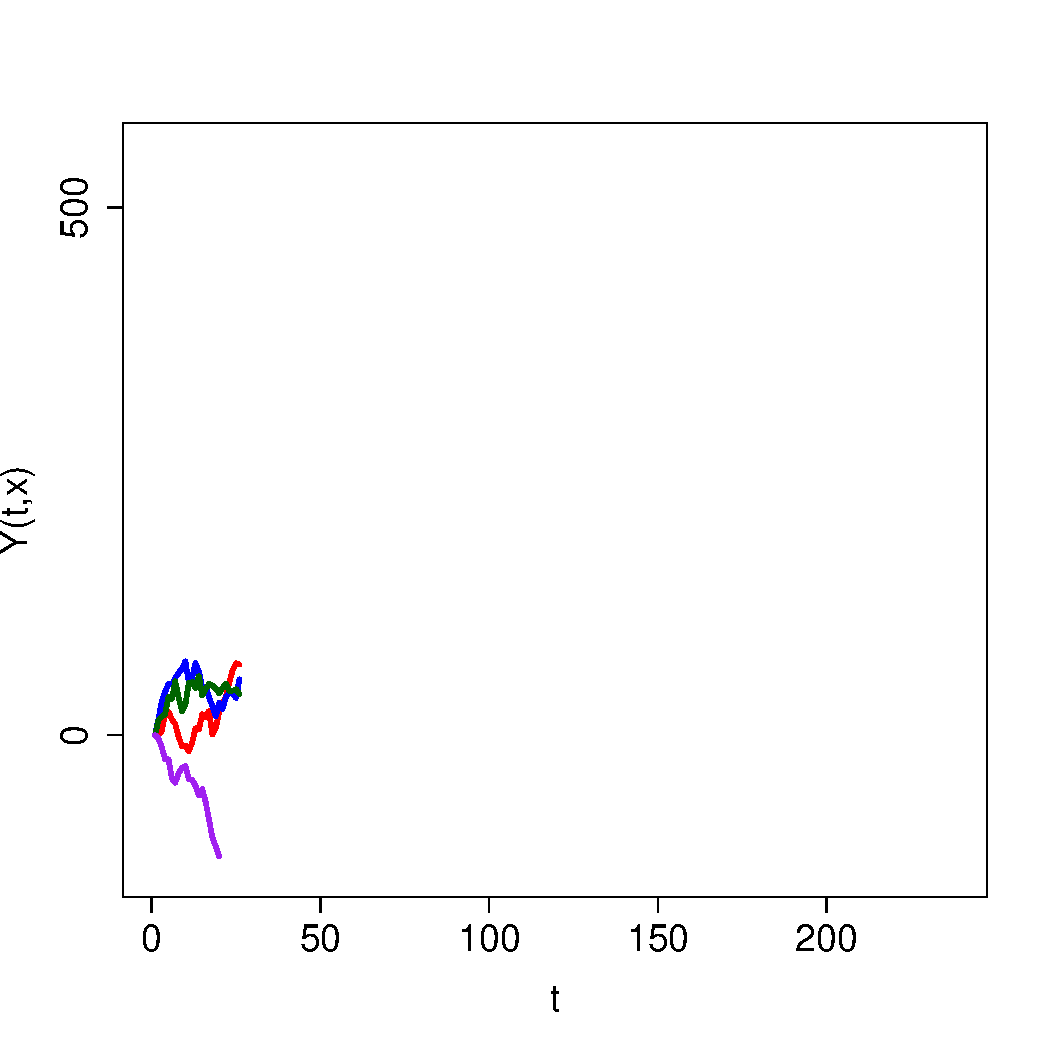
\includegraphics[height=\textheight]{\figdir/biz/AFOSR2013/animation/pdf2/animation_0026.pdf}\end{figure}\end{frame}
\begin{frame}\frametitle{A Typical Ranking \& Selection Procedure}\begin{figure}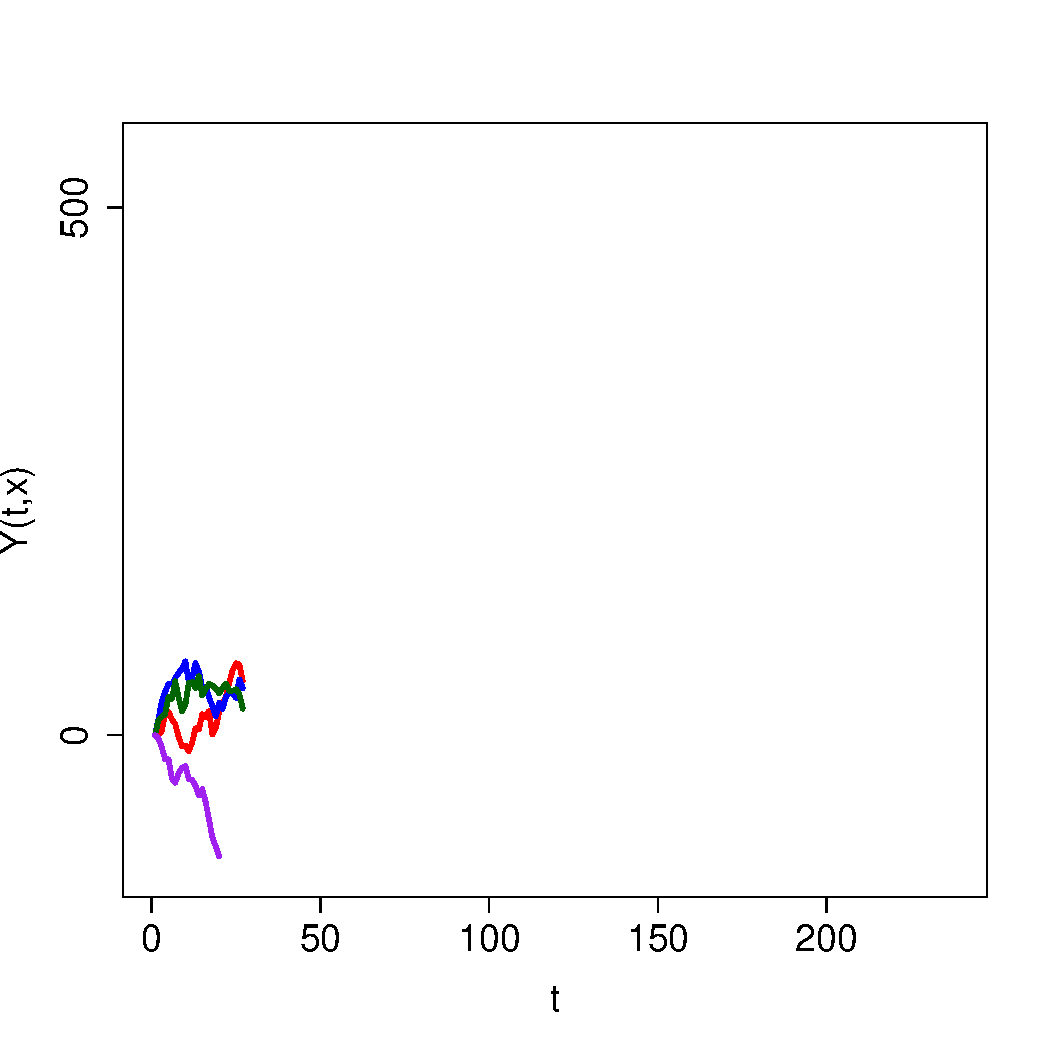
\includegraphics[height=\textheight]{\figdir/biz/AFOSR2013/animation/pdf2/animation_0027.pdf}\end{figure}\end{frame}
\begin{frame}\frametitle{A Typical Ranking \& Selection Procedure}\begin{figure}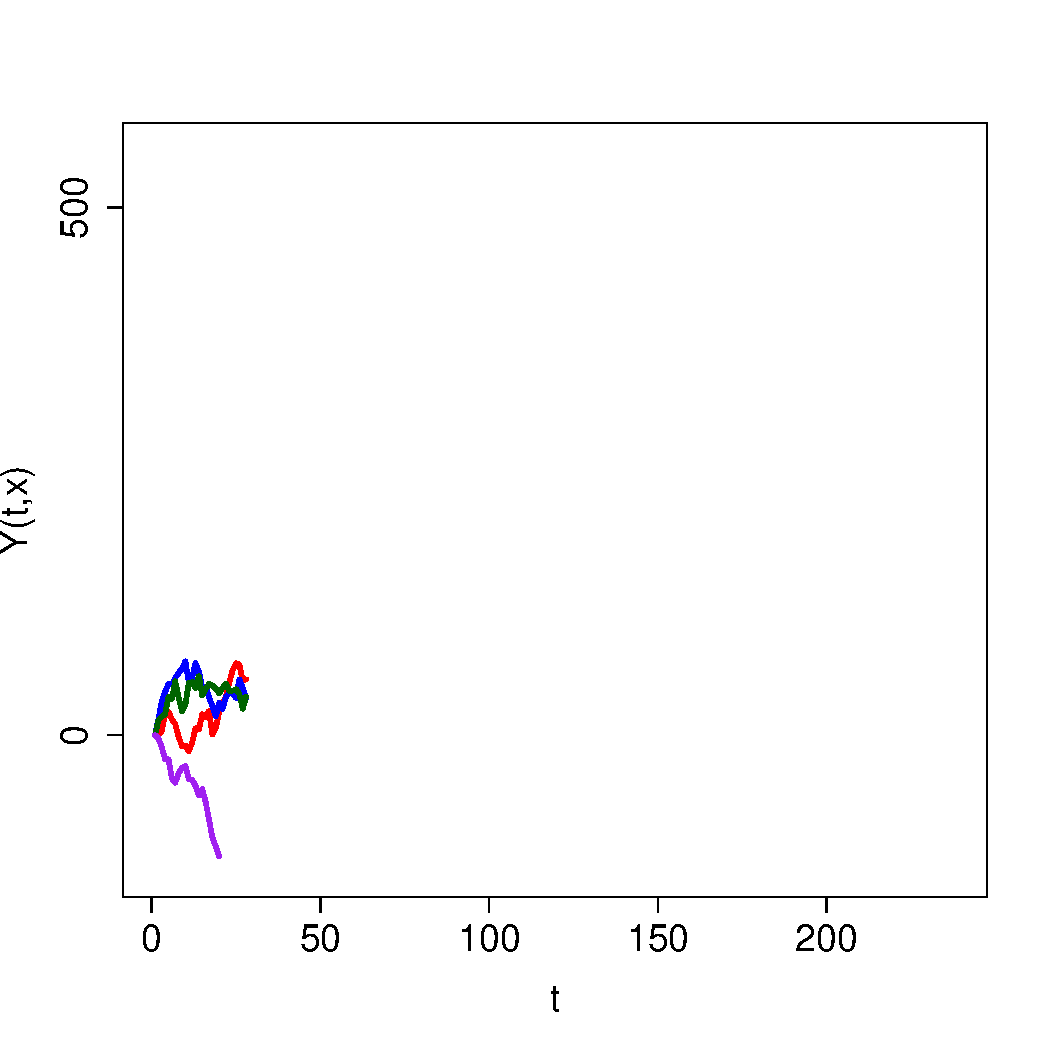
\includegraphics[height=\textheight]{\figdir/biz/AFOSR2013/animation/pdf2/animation_0028.pdf}\end{figure}\end{frame}
\begin{frame}\frametitle{A Typical Ranking \& Selection Procedure}\begin{figure}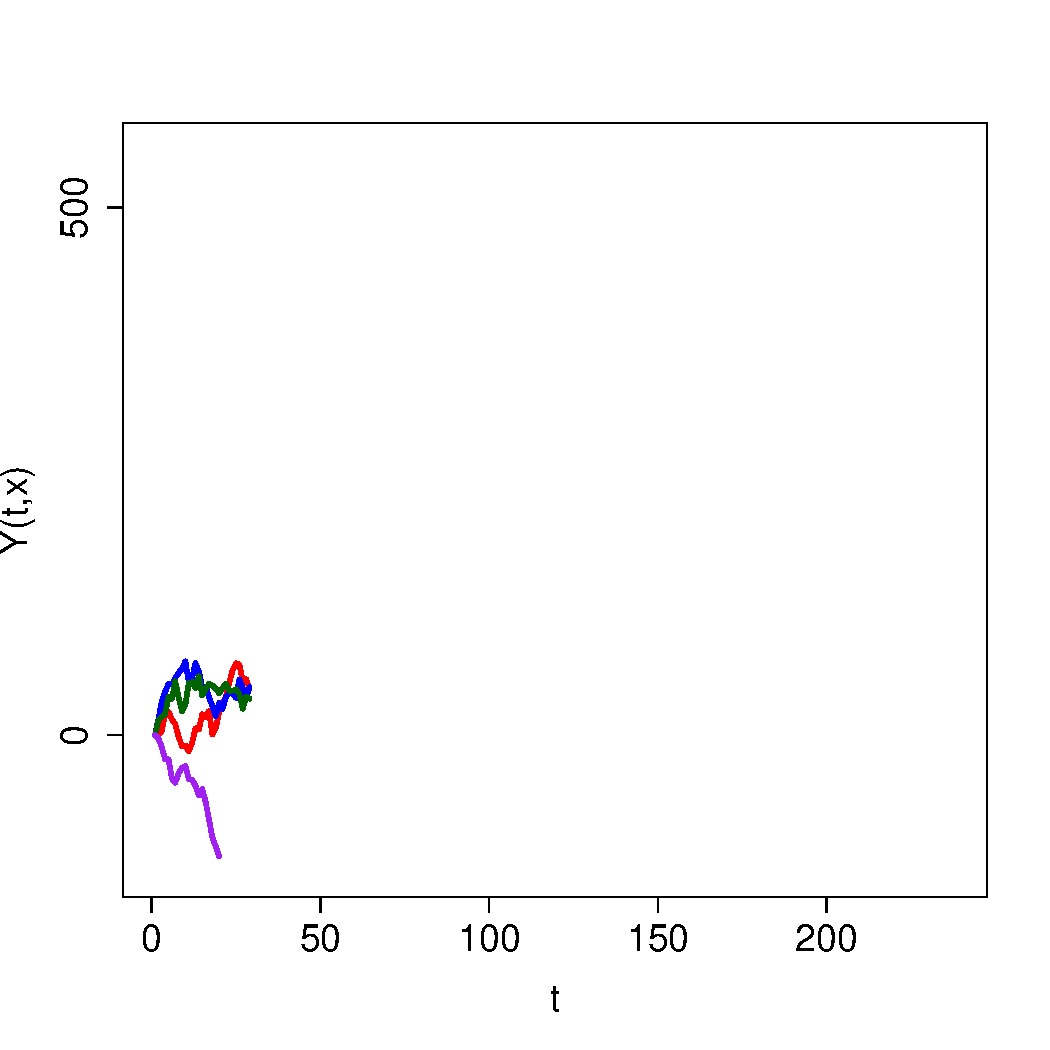
\includegraphics[height=\textheight]{\figdir/biz/AFOSR2013/animation/pdf2/animation_0029.pdf}\end{figure}\end{frame}
\begin{frame}\frametitle{A Typical Ranking \& Selection Procedure}\begin{figure}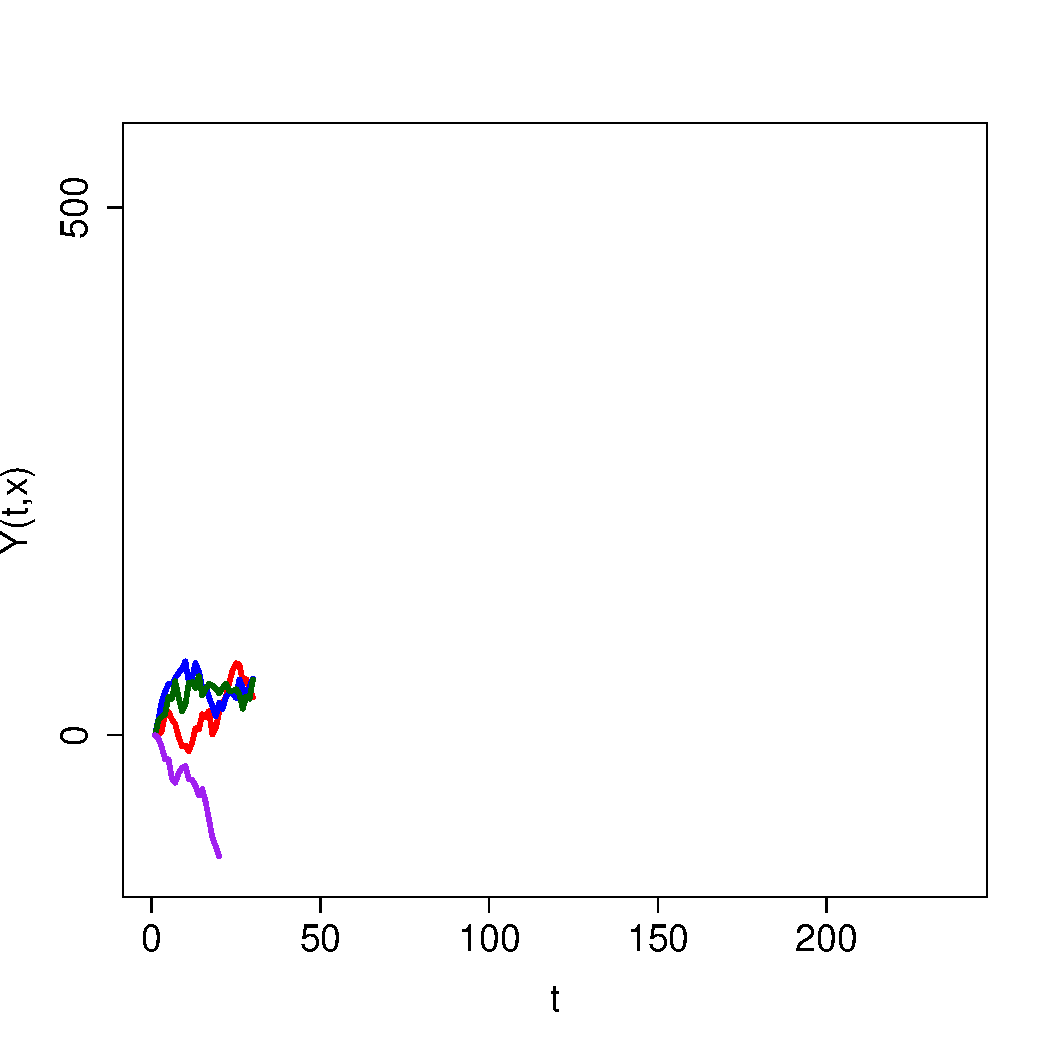
\includegraphics[height=\textheight]{\figdir/biz/AFOSR2013/animation/pdf2/animation_0030.pdf}\end{figure}\end{frame}
\begin{frame}\frametitle{A Typical Ranking \& Selection Procedure}\begin{figure}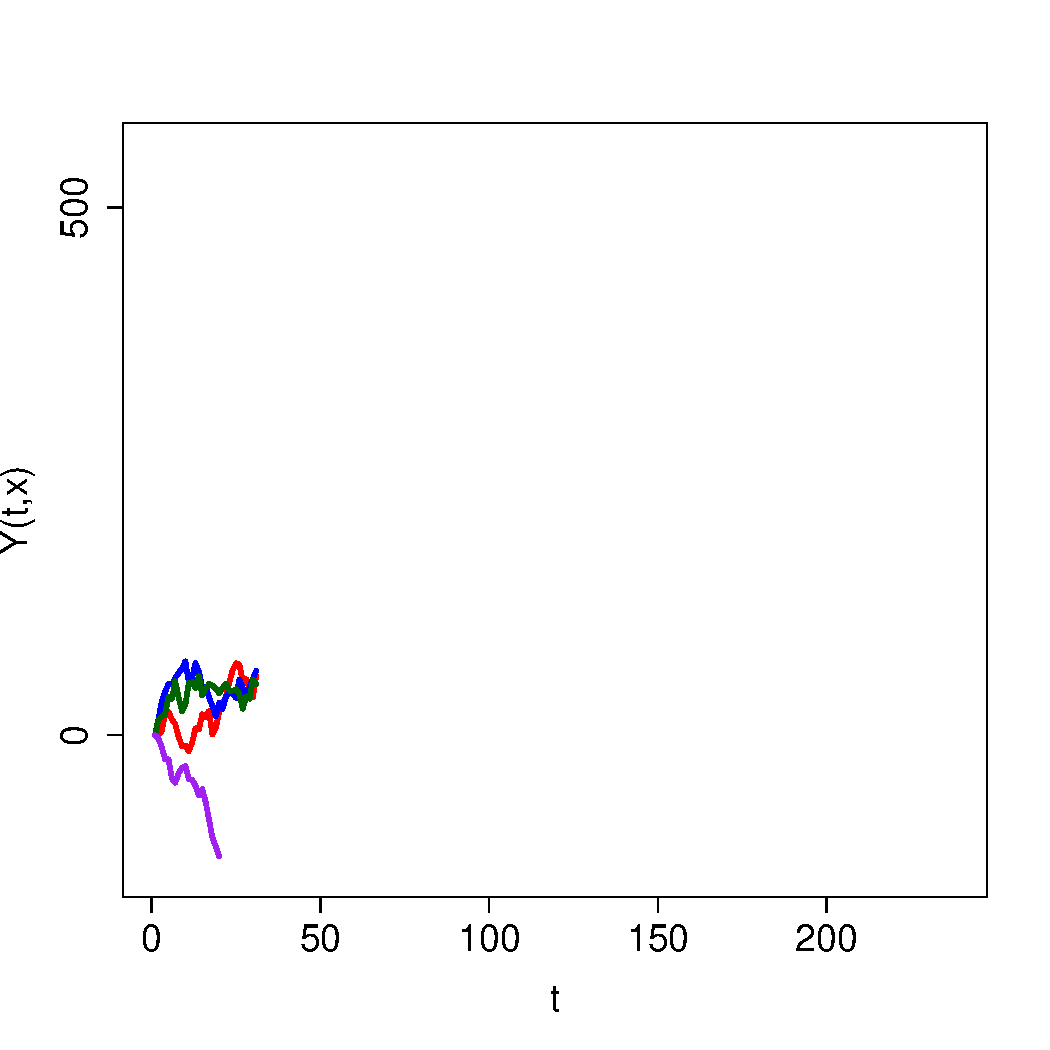
\includegraphics[height=\textheight]{\figdir/biz/AFOSR2013/animation/pdf2/animation_0031.pdf}\end{figure}\end{frame}
\begin{frame}\frametitle{A Typical Ranking \& Selection Procedure}\begin{figure}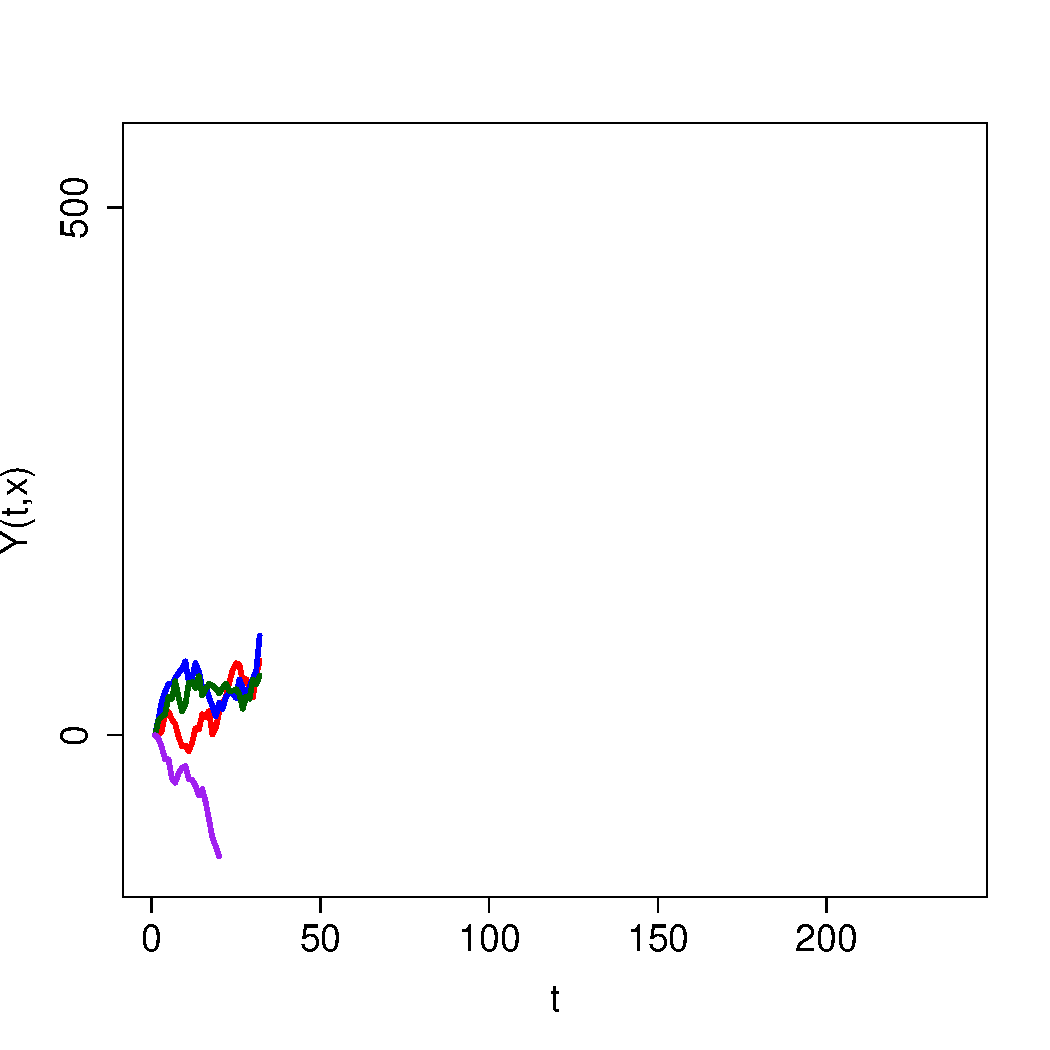
\includegraphics[height=\textheight]{\figdir/biz/AFOSR2013/animation/pdf2/animation_0032.pdf}\end{figure}\end{frame}
\begin{frame}\frametitle{A Typical Ranking \& Selection Procedure}\begin{figure}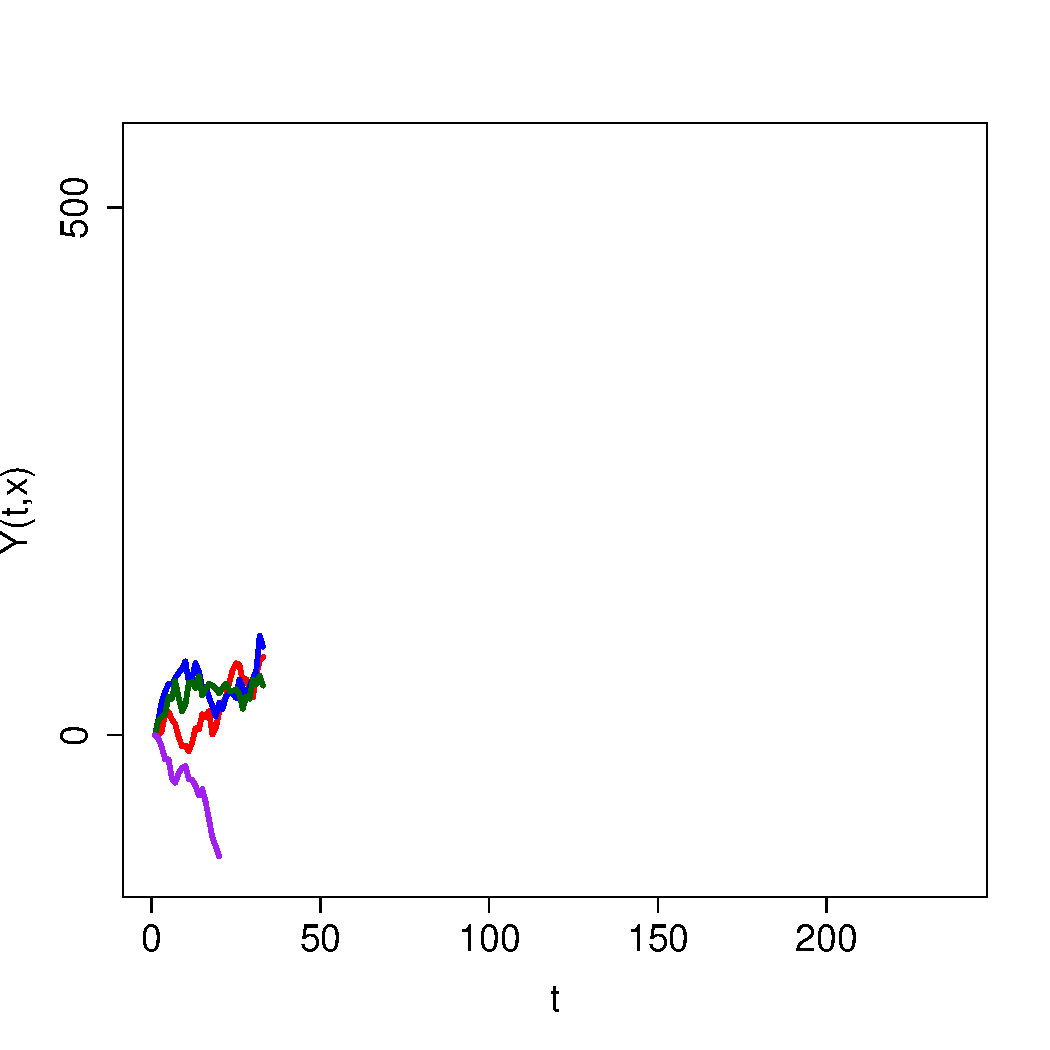
\includegraphics[height=\textheight]{\figdir/biz/AFOSR2013/animation/pdf2/animation_0033.pdf}\end{figure}\end{frame}
\begin{frame}\frametitle{A Typical Ranking \& Selection Procedure}\begin{figure}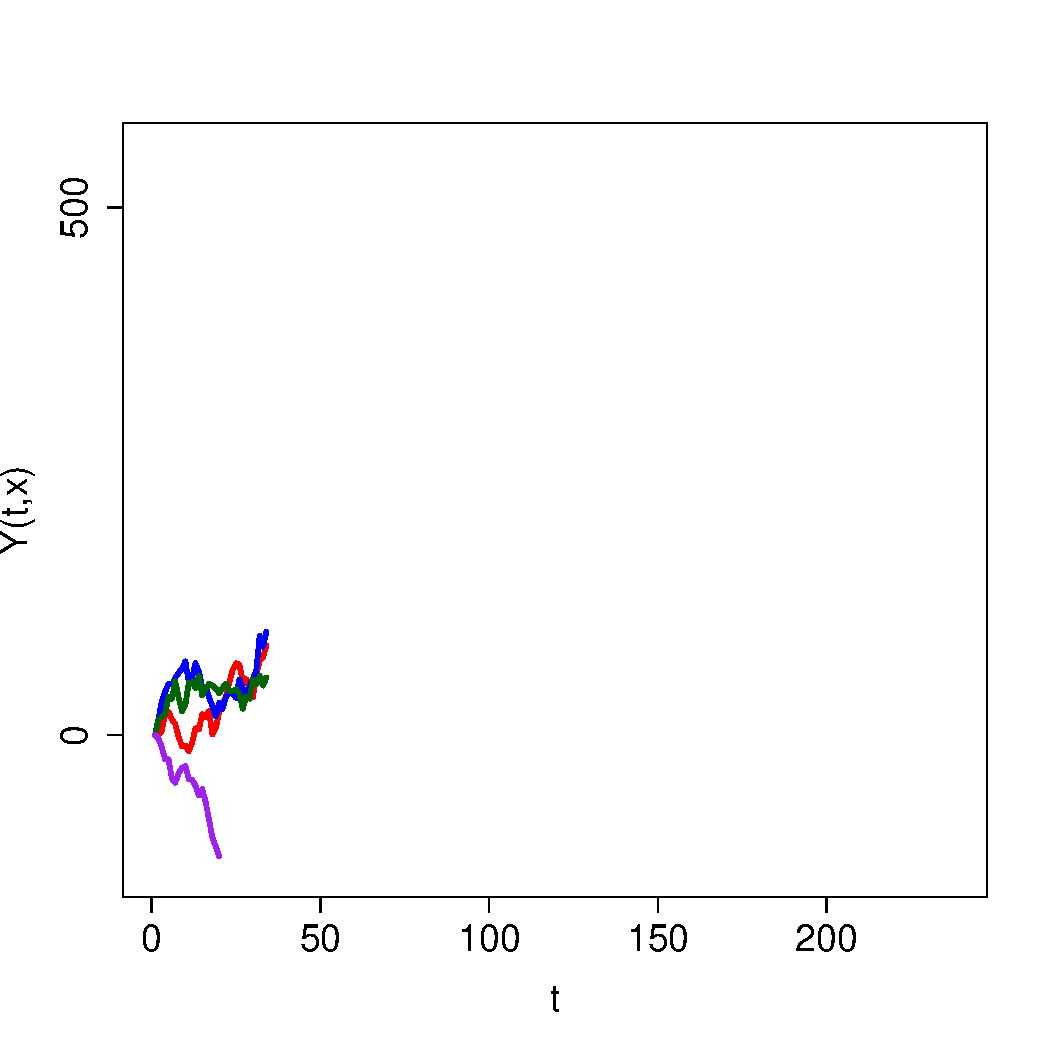
\includegraphics[height=\textheight]{\figdir/biz/AFOSR2013/animation/pdf2/animation_0034.pdf}\end{figure}\end{frame}
\begin{frame}\frametitle{A Typical Ranking \& Selection Procedure}\begin{figure}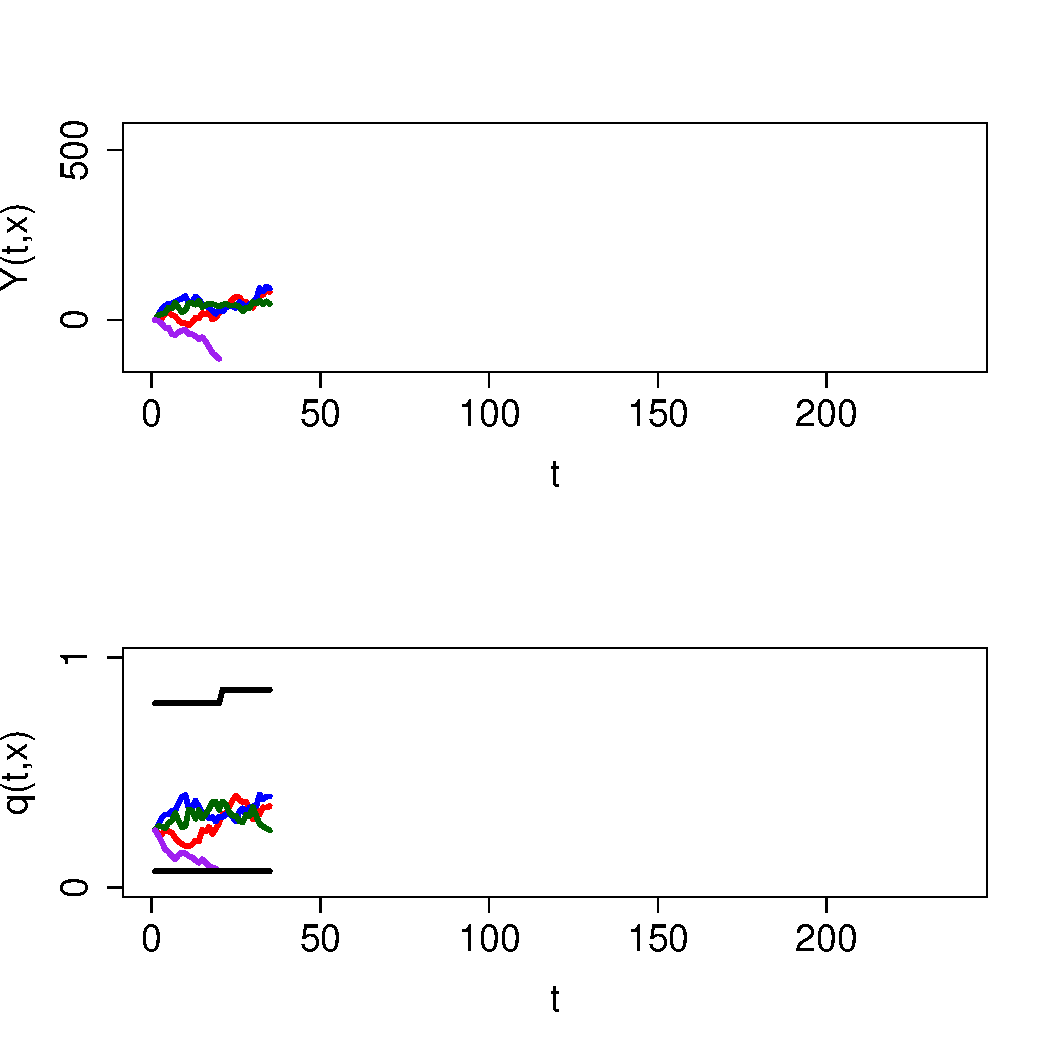
\includegraphics[height=\textheight]{\figdir/biz/AFOSR2013/animation/pdf2/animation_0035.pdf}\end{figure}\end{frame}
\begin{frame}\frametitle{A Typical Ranking \& Selection Procedure}\begin{figure}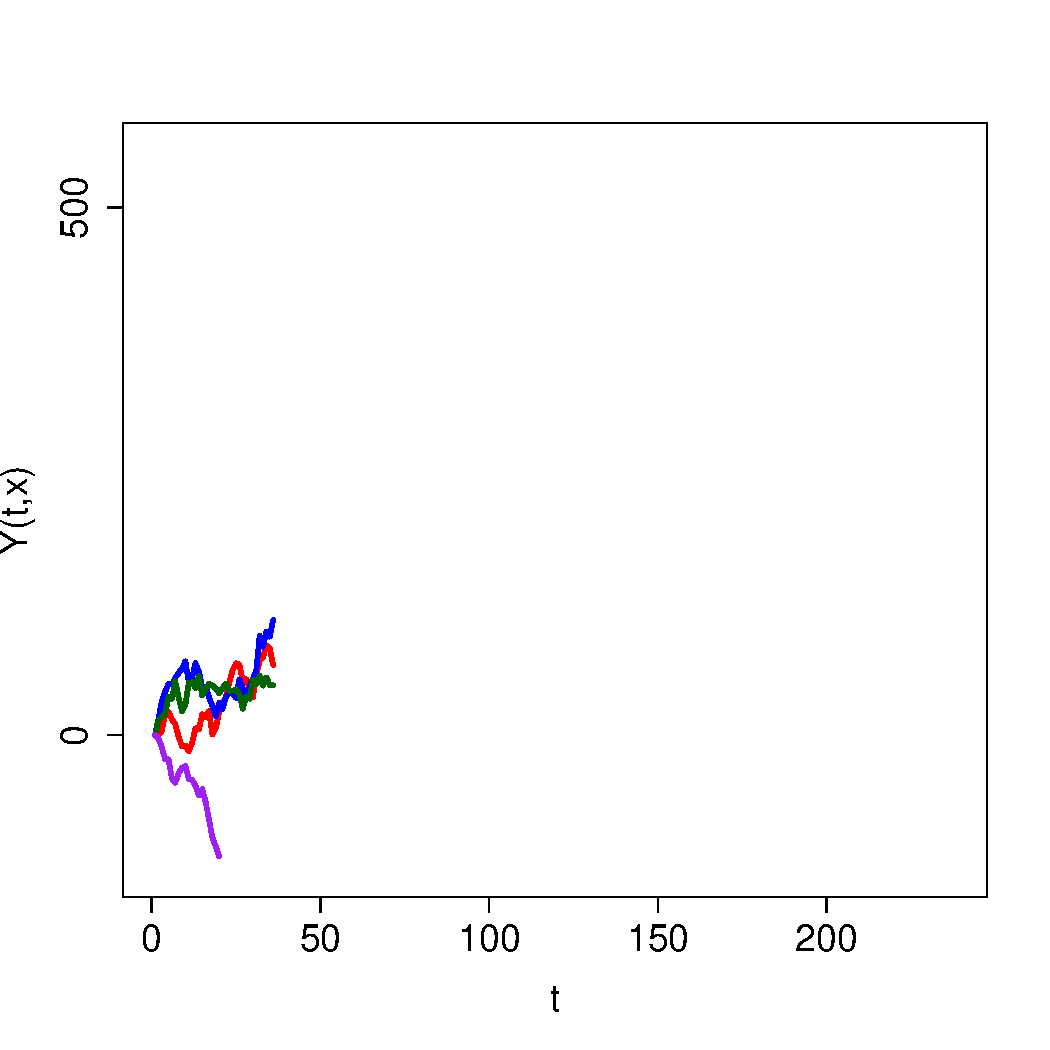
\includegraphics[height=\textheight]{\figdir/biz/AFOSR2013/animation/pdf2/animation_0036.pdf}\end{figure}\end{frame}
\begin{frame}\frametitle{A Typical Ranking \& Selection Procedure}\begin{figure}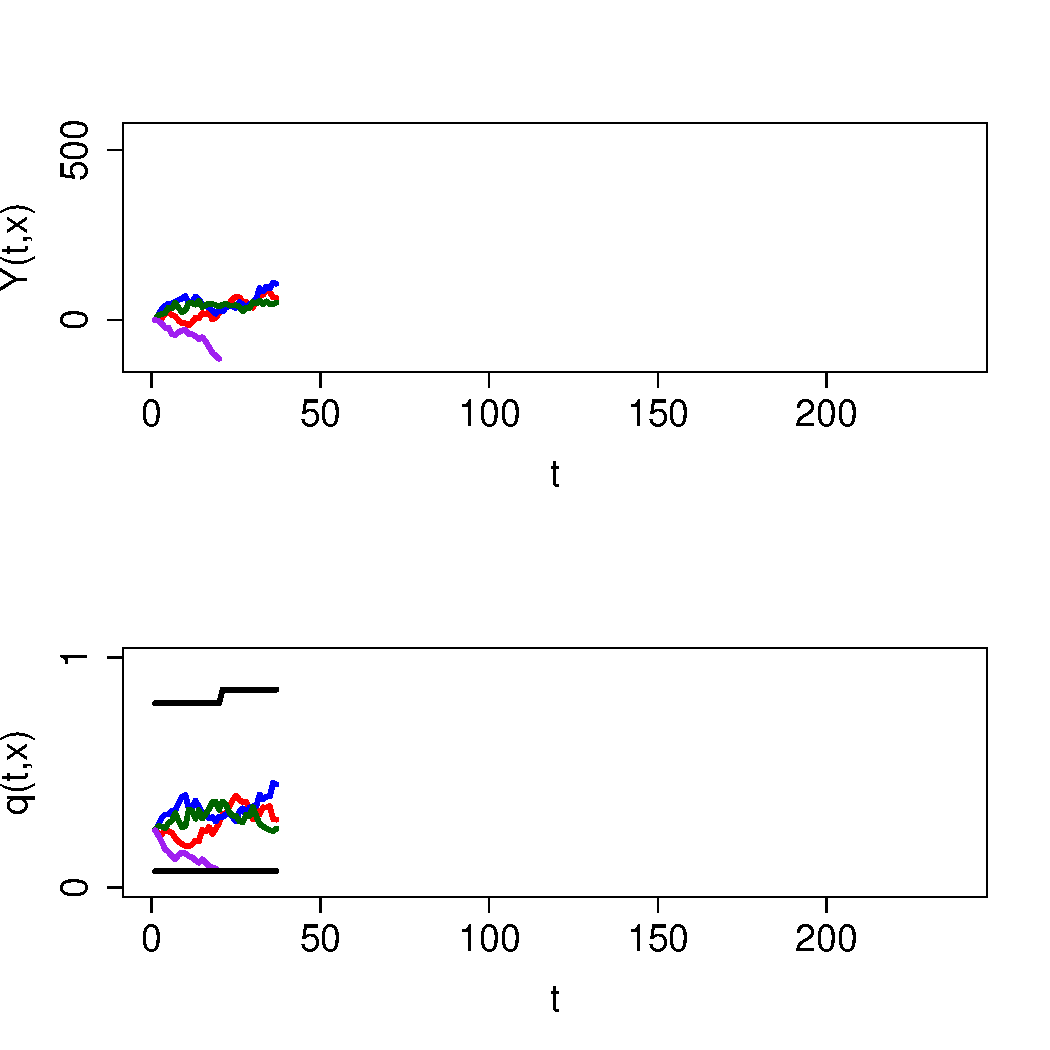
\includegraphics[height=\textheight]{\figdir/biz/AFOSR2013/animation/pdf2/animation_0037.pdf}\end{figure}\end{frame}
\begin{frame}\frametitle{A Typical Ranking \& Selection Procedure}\begin{figure}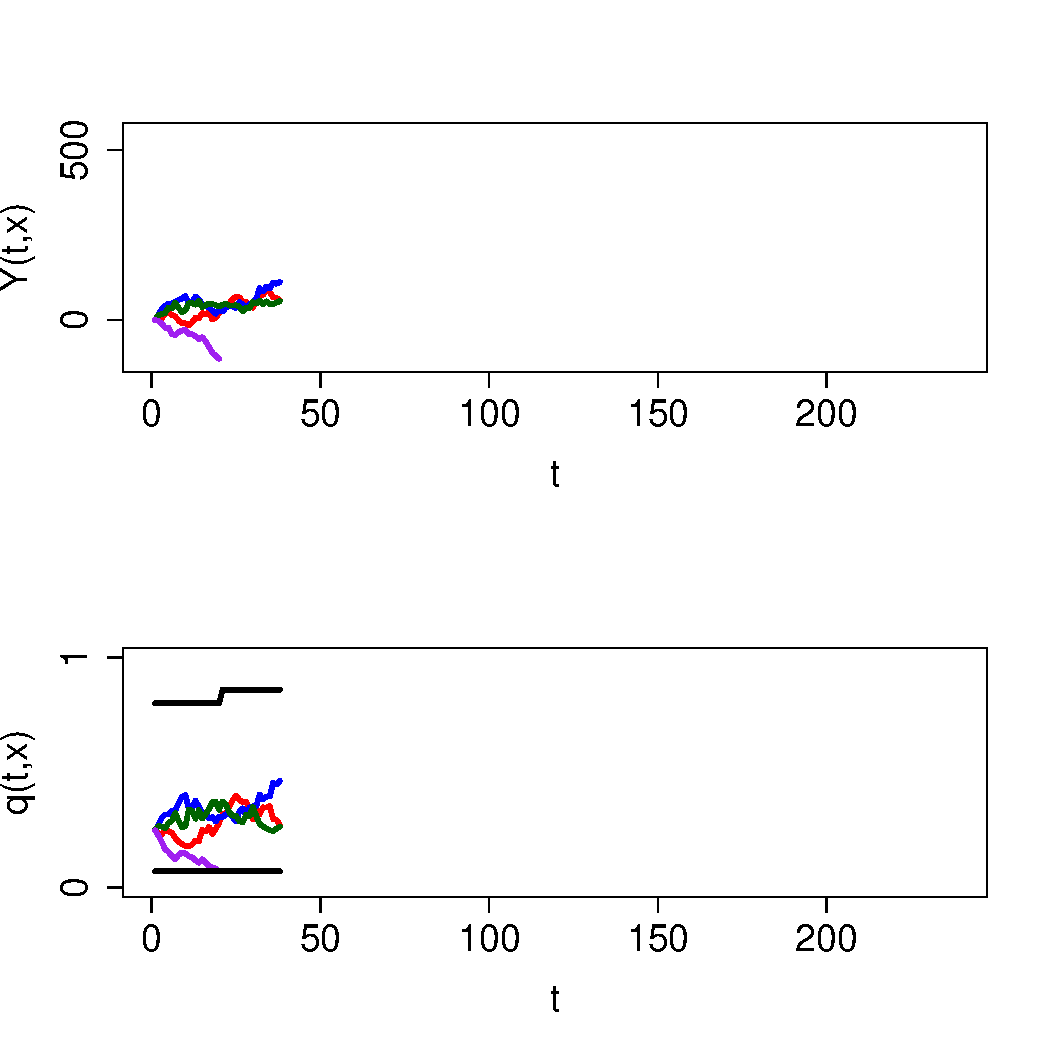
\includegraphics[height=\textheight]{\figdir/biz/AFOSR2013/animation/pdf2/animation_0038.pdf}\end{figure}\end{frame}
\begin{frame}\frametitle{A Typical Ranking \& Selection Procedure}\begin{figure}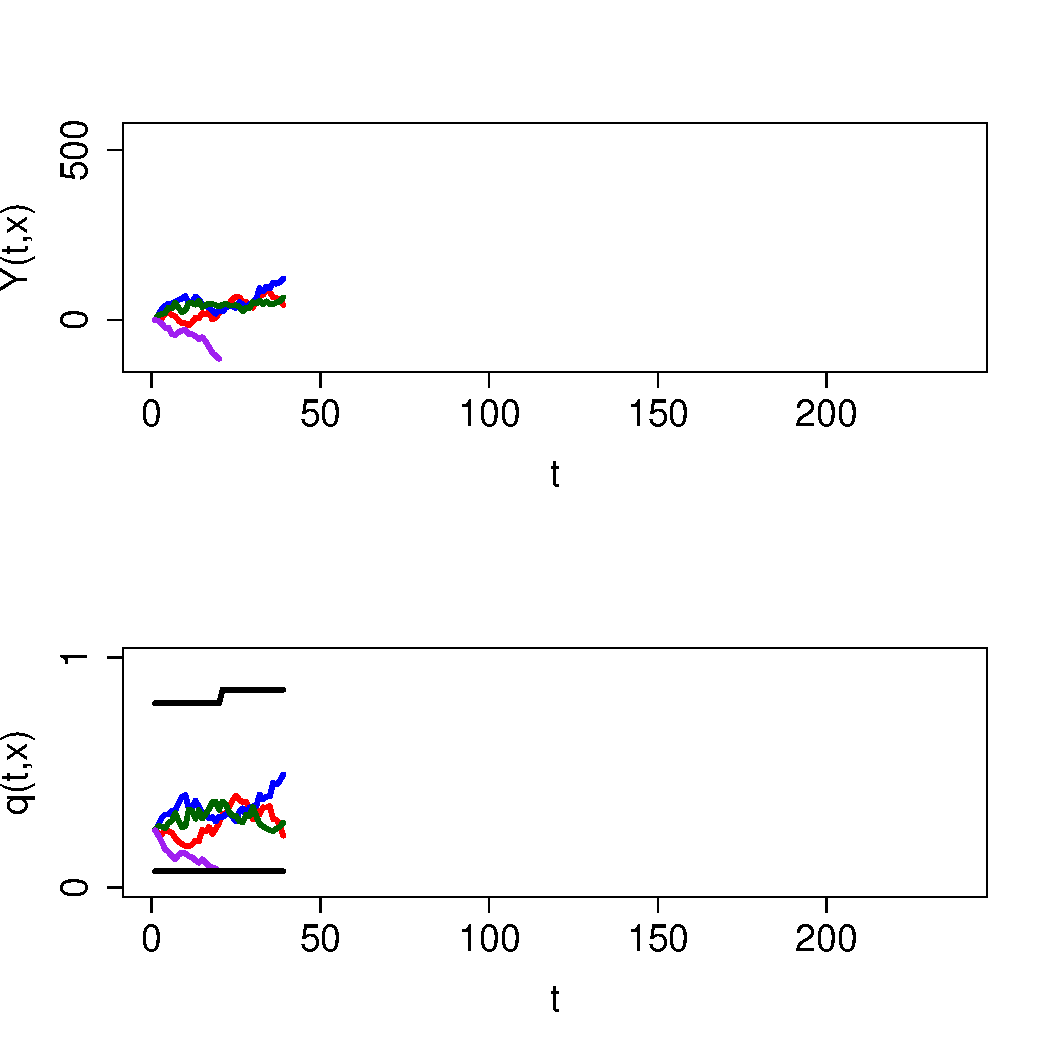
\includegraphics[height=\textheight]{\figdir/biz/AFOSR2013/animation/pdf2/animation_0039.pdf}\end{figure}\end{frame}
\begin{frame}\frametitle{A Typical Ranking \& Selection Procedure}\begin{figure}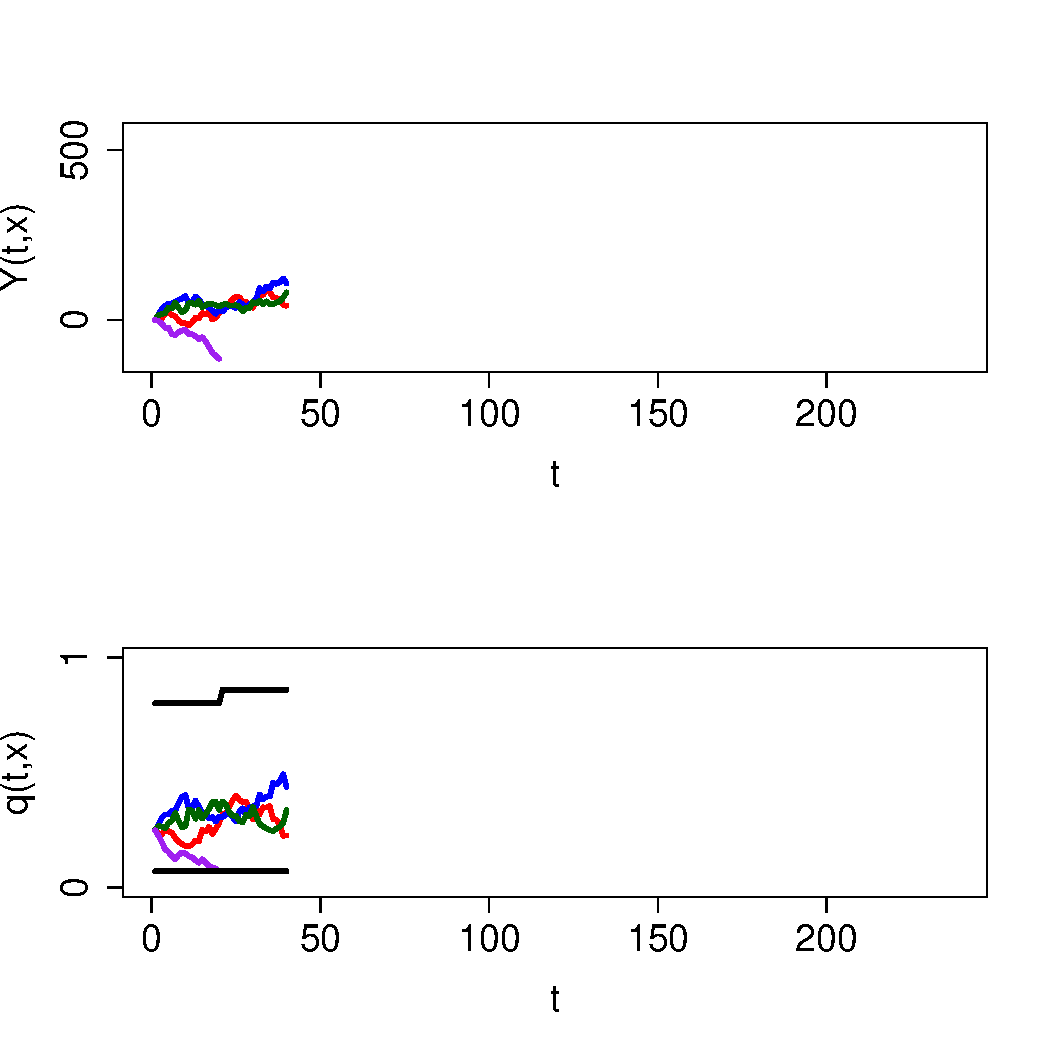
\includegraphics[height=\textheight]{\figdir/biz/AFOSR2013/animation/pdf2/animation_0040.pdf}\end{figure}\end{frame}
\begin{frame}\frametitle{A Typical Ranking \& Selection Procedure}\begin{figure}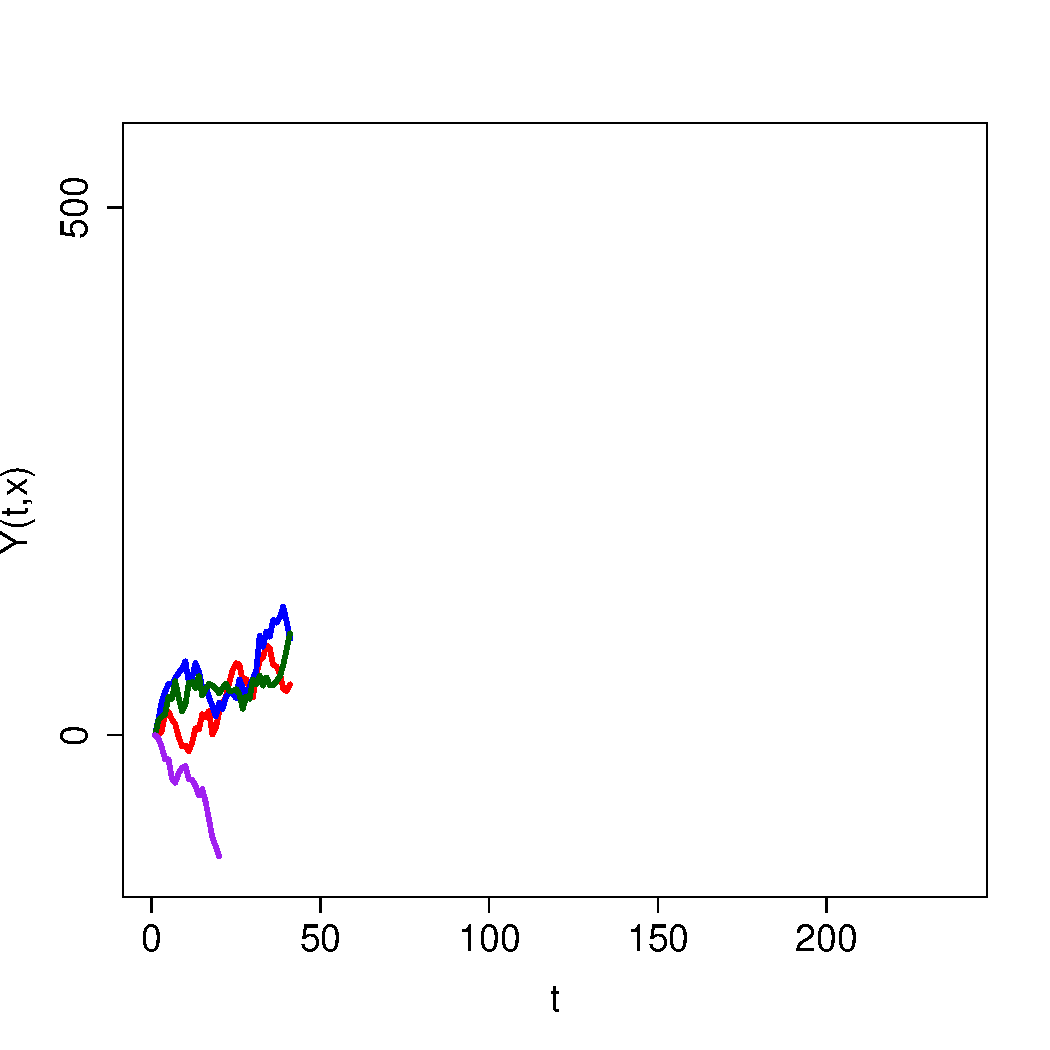
\includegraphics[height=\textheight]{\figdir/biz/AFOSR2013/animation/pdf2/animation_0041.pdf}\end{figure}\end{frame}
\begin{frame}\frametitle{A Typical Ranking \& Selection Procedure}\begin{figure}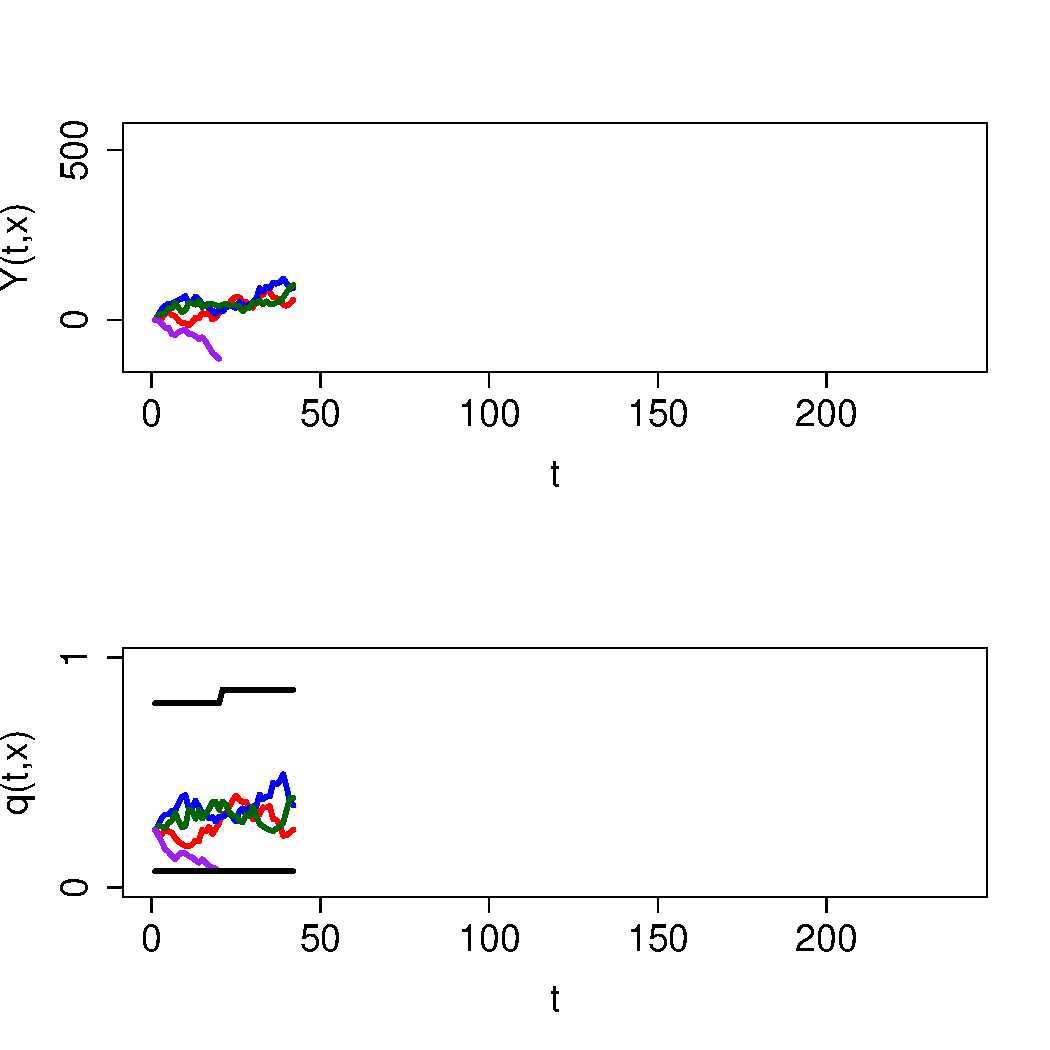
\includegraphics[height=\textheight]{\figdir/biz/AFOSR2013/animation/pdf2/animation_0042.pdf}\end{figure}\end{frame}
\begin{frame}\frametitle{A Typical Ranking \& Selection Procedure}\begin{figure}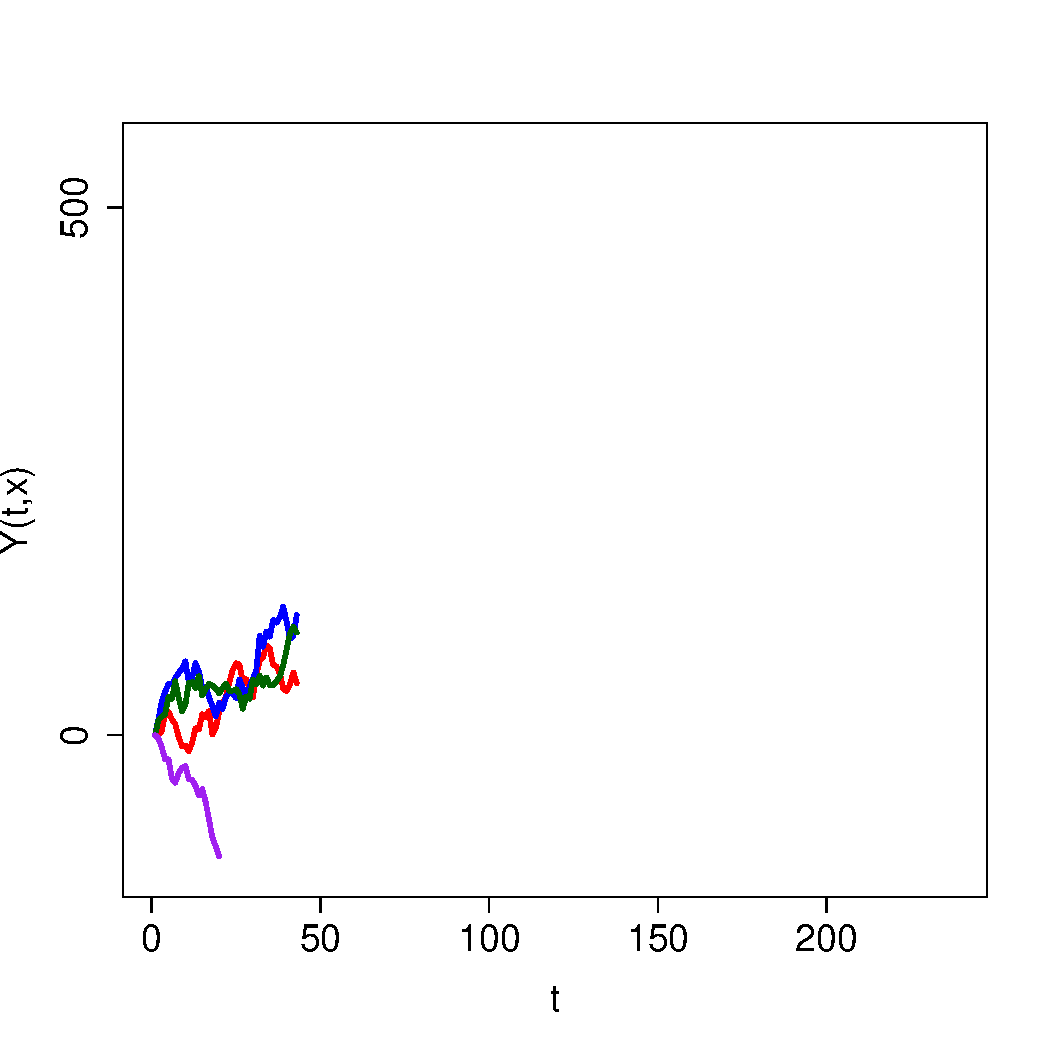
\includegraphics[height=\textheight]{\figdir/biz/AFOSR2013/animation/pdf2/animation_0043.pdf}\end{figure}\end{frame}
\begin{frame}\frametitle{A Typical Ranking \& Selection Procedure}\begin{figure}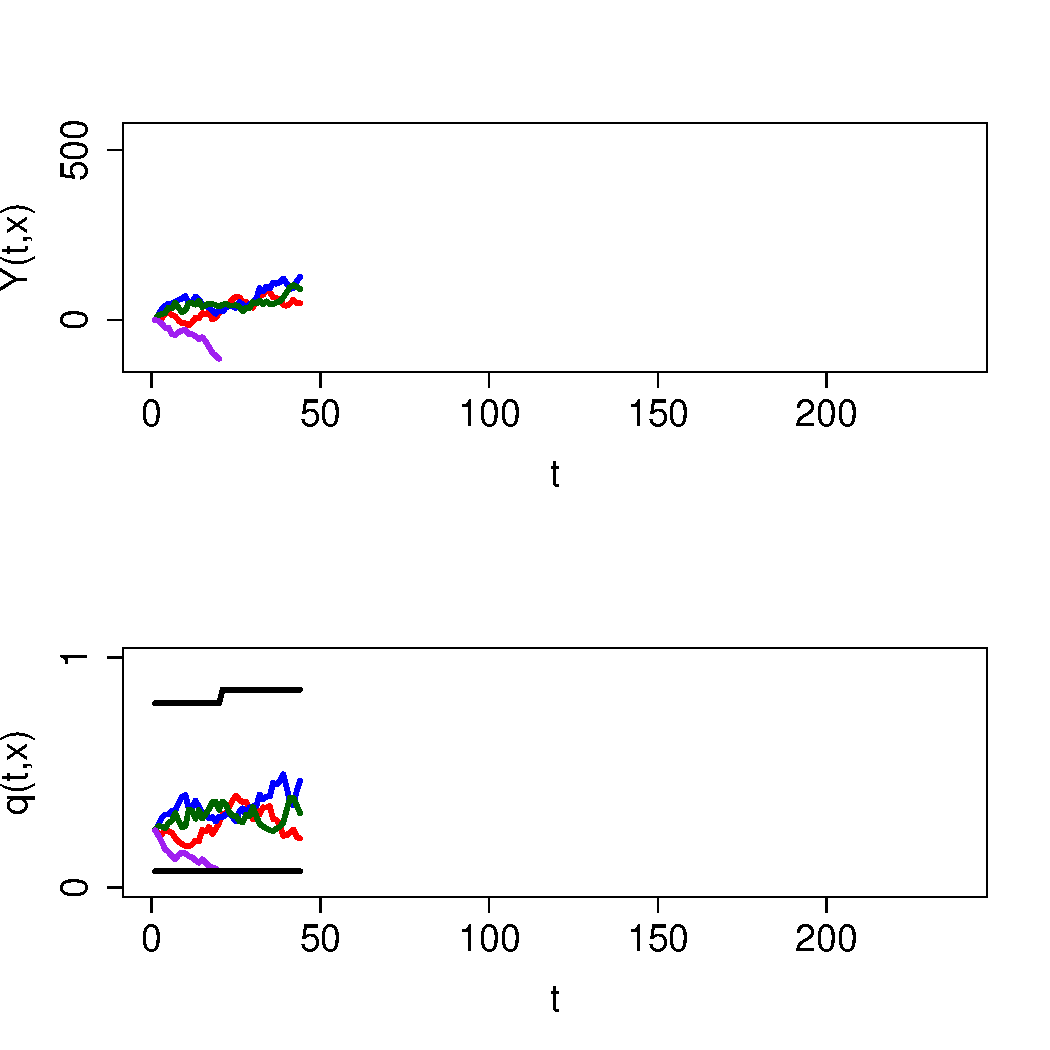
\includegraphics[height=\textheight]{\figdir/biz/AFOSR2013/animation/pdf2/animation_0044.pdf}\end{figure}\end{frame}
\begin{frame}\frametitle{A Typical Ranking \& Selection Procedure}\begin{figure}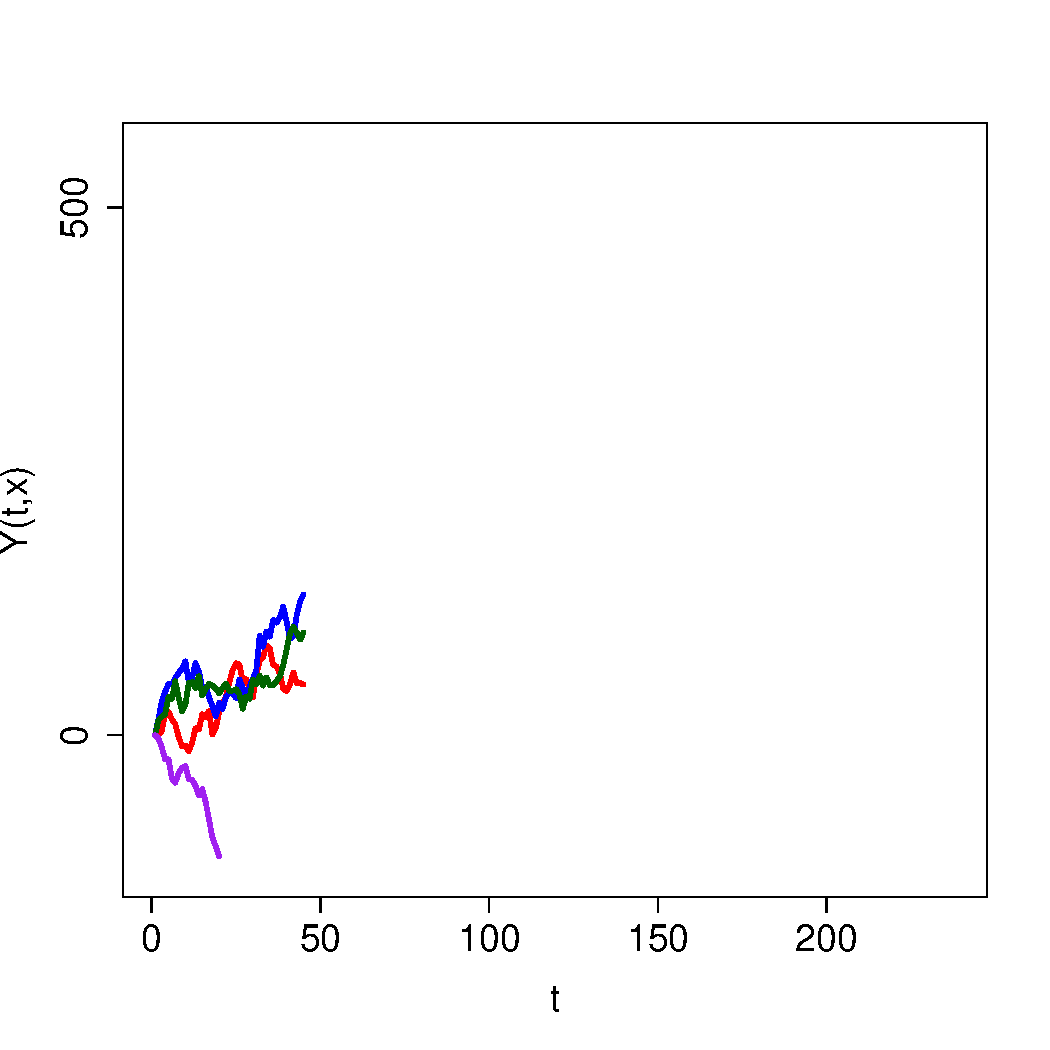
\includegraphics[height=\textheight]{\figdir/biz/AFOSR2013/animation/pdf2/animation_0045.pdf}\end{figure}\end{frame}
\begin{frame}\frametitle{A Typical Ranking \& Selection Procedure}\begin{figure}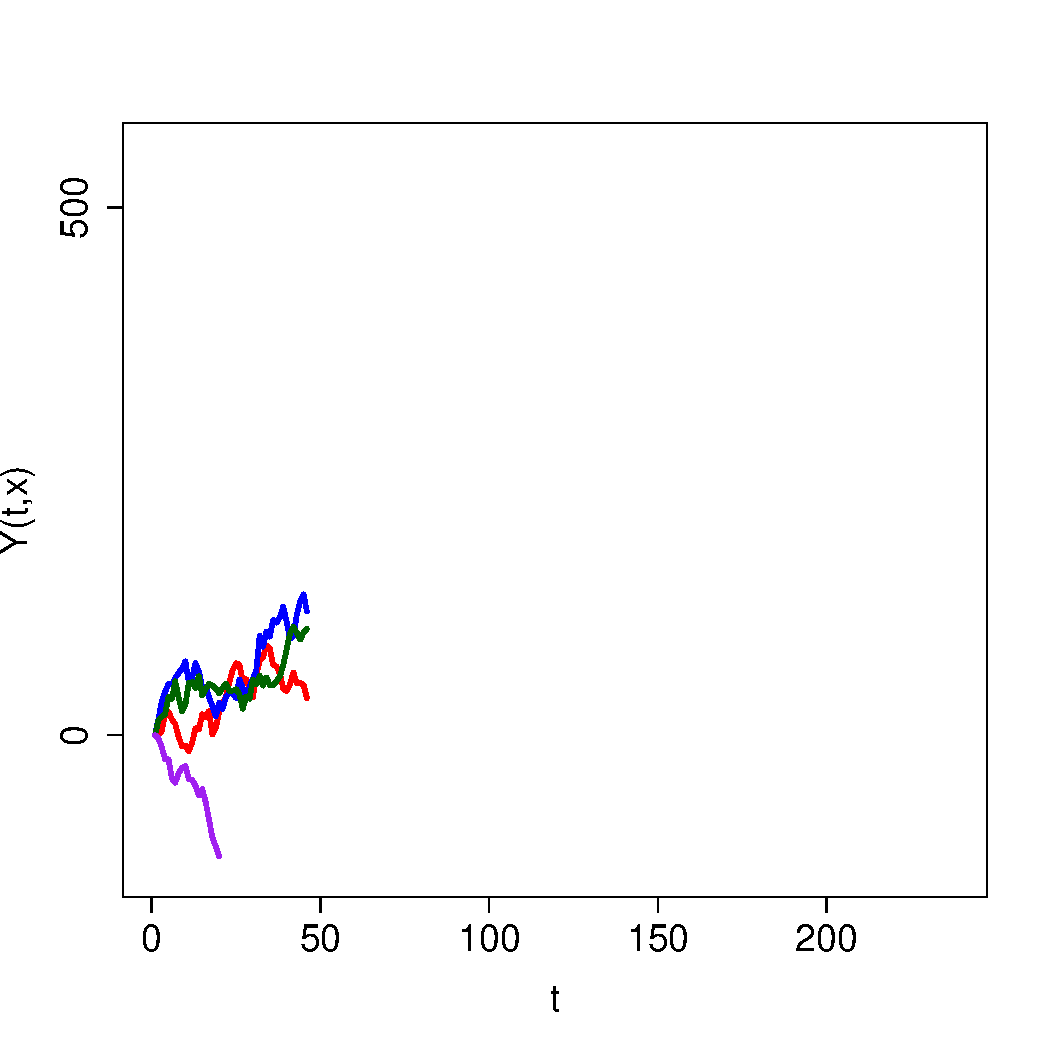
\includegraphics[height=\textheight]{\figdir/biz/AFOSR2013/animation/pdf2/animation_0046.pdf}\end{figure}\end{frame}
\begin{frame}\frametitle{A Typical Ranking \& Selection Procedure}\begin{figure}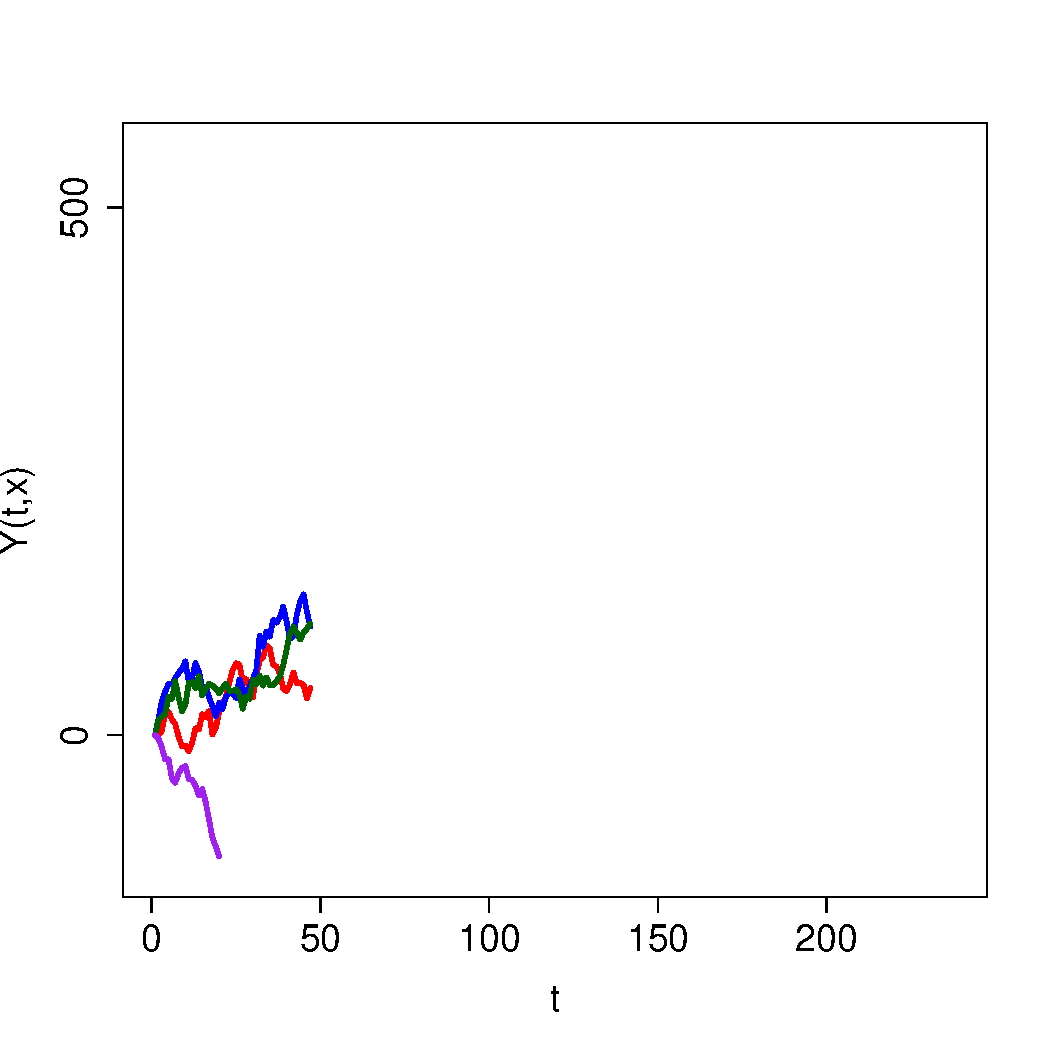
\includegraphics[height=\textheight]{\figdir/biz/AFOSR2013/animation/pdf2/animation_0047.pdf}\end{figure}\end{frame}
\begin{frame}\frametitle{A Typical Ranking \& Selection Procedure}\begin{figure}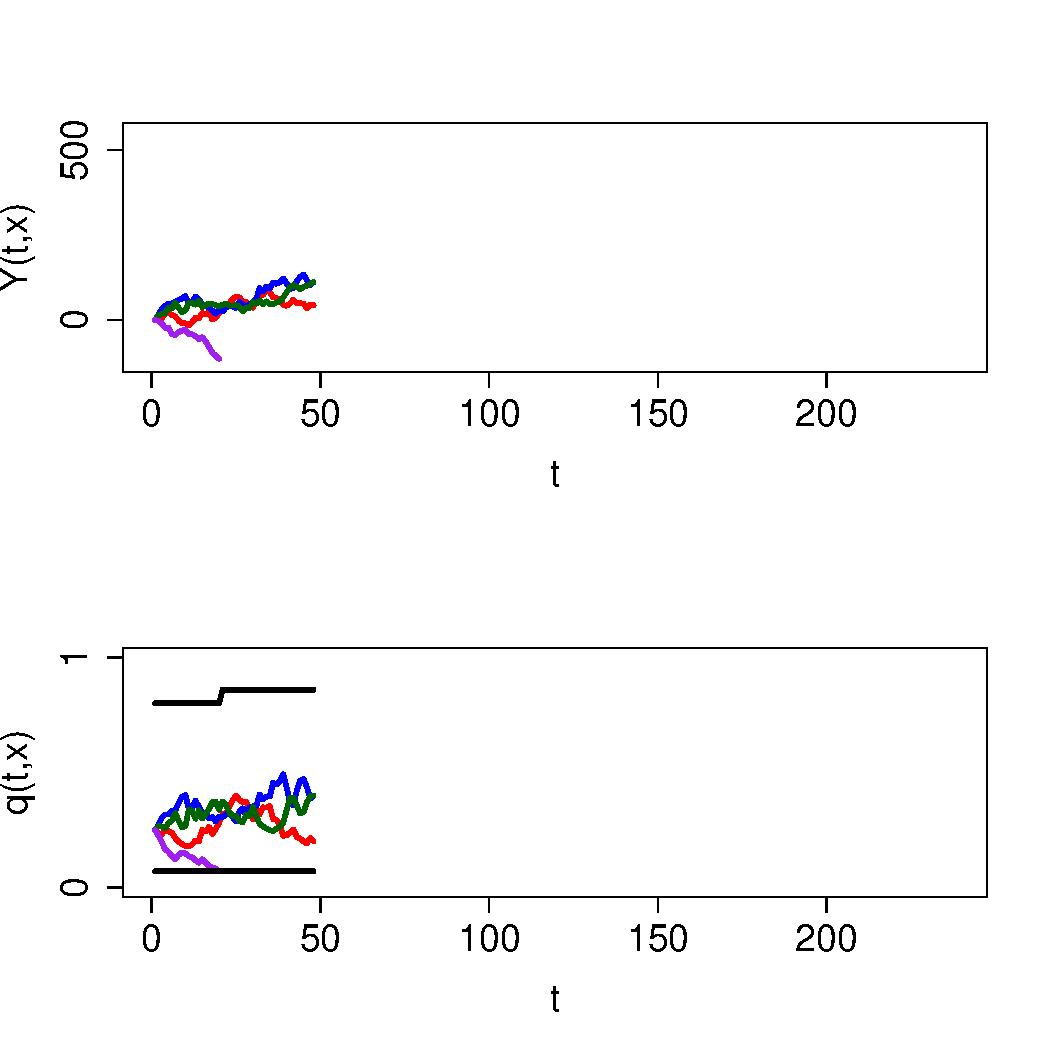
\includegraphics[height=\textheight]{\figdir/biz/AFOSR2013/animation/pdf2/animation_0048.pdf}\end{figure}\end{frame}
\begin{frame}\frametitle{A Typical Ranking \& Selection Procedure}\begin{figure}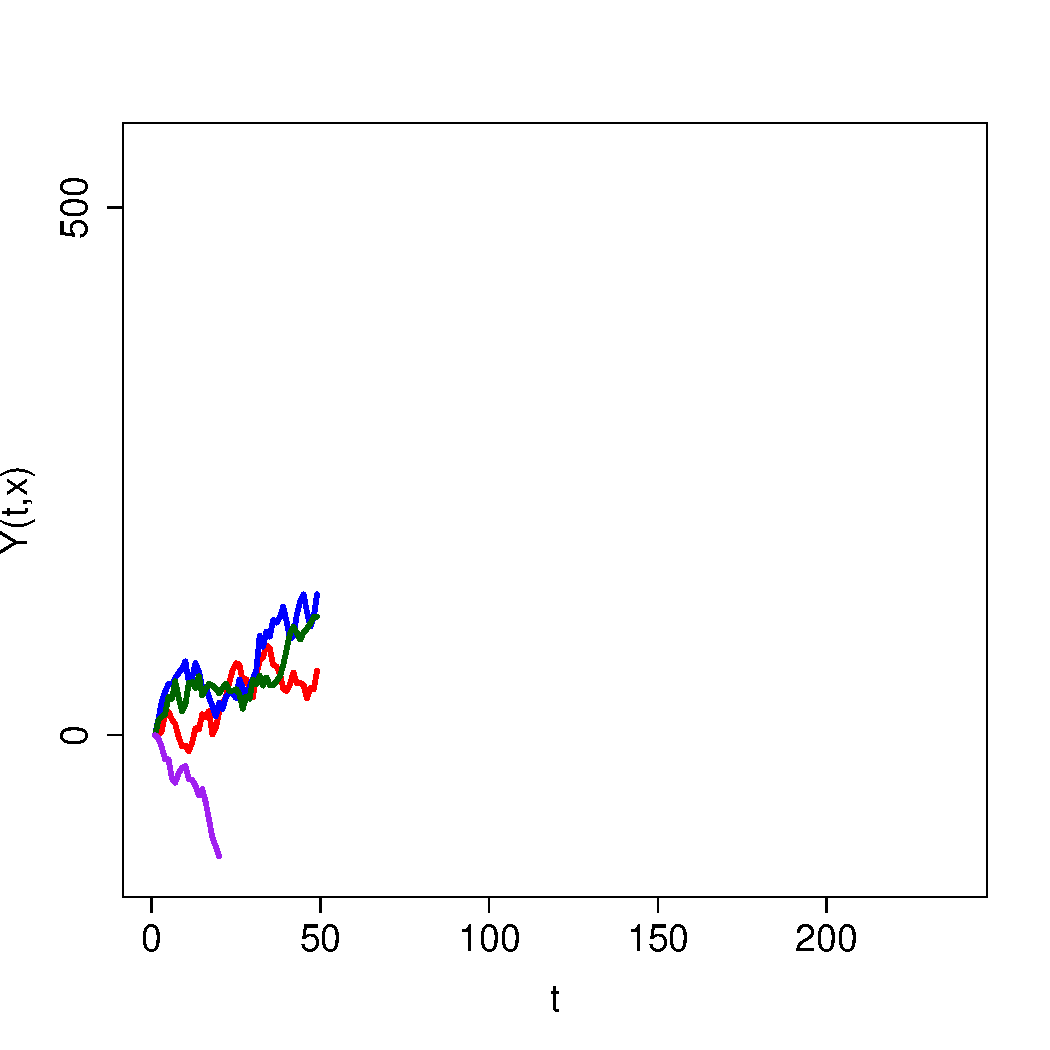
\includegraphics[height=\textheight]{\figdir/biz/AFOSR2013/animation/pdf2/animation_0049.pdf}\end{figure}\end{frame}
\begin{frame}\frametitle{A Typical Ranking \& Selection Procedure}\begin{figure}\includegraphics[height=\textheight]{\figdir/biz/AFOSR2013/animation/pdf2/animation_0050.pdf}\end{figure}\end{frame}
\begin{frame}\frametitle{A Typical Ranking \& Selection Procedure}\begin{figure}\includegraphics[height=\textheight]{\figdir/biz/AFOSR2013/animation/pdf2/animation_0051.pdf}\end{figure}\end{frame}
\begin{frame}\frametitle{A Typical Ranking \& Selection Procedure}\begin{figure}\includegraphics[height=\textheight]{\figdir/biz/AFOSR2013/animation/pdf2/animation_0052.pdf}\end{figure}\end{frame}
\begin{frame}\frametitle{A Typical Ranking \& Selection Procedure}\begin{figure}\includegraphics[height=\textheight]{\figdir/biz/AFOSR2013/animation/pdf2/animation_0053.pdf}\end{figure}\end{frame}
\begin{frame}\frametitle{A Typical Ranking \& Selection Procedure}\begin{figure}\includegraphics[height=\textheight]{\figdir/biz/AFOSR2013/animation/pdf2/animation_0054.pdf}\end{figure}\end{frame}
\begin{frame}\frametitle{A Typical Ranking \& Selection Procedure}\begin{figure}\includegraphics[height=\textheight]{\figdir/biz/AFOSR2013/animation/pdf2/animation_0055.pdf}\end{figure}\end{frame}
\begin{frame}\frametitle{A Typical Ranking \& Selection Procedure}\begin{figure}\includegraphics[height=\textheight]{\figdir/biz/AFOSR2013/animation/pdf2/animation_0056.pdf}\end{figure}\end{frame}
\begin{frame}\frametitle{A Typical Ranking \& Selection Procedure}\begin{figure}\includegraphics[height=\textheight]{\figdir/biz/AFOSR2013/animation/pdf2/animation_0057.pdf}\end{figure}\end{frame}
\begin{frame}\frametitle{A Typical Ranking \& Selection Procedure}\begin{figure}\includegraphics[height=\textheight]{\figdir/biz/AFOSR2013/animation/pdf2/animation_0058.pdf}\end{figure}\end{frame}
\begin{frame}\frametitle{A Typical Ranking \& Selection Procedure}\begin{figure}\includegraphics[height=\textheight]{\figdir/biz/AFOSR2013/animation/pdf2/animation_0059.pdf}\end{figure}\end{frame}
\begin{frame}\frametitle{A Typical Ranking \& Selection Procedure}\begin{figure}\includegraphics[height=\textheight]{\figdir/biz/AFOSR2013/animation/pdf2/animation_0060.pdf}\end{figure}\end{frame}
\begin{frame}\frametitle{A Typical Ranking \& Selection Procedure}\begin{figure}\includegraphics[height=\textheight]{\figdir/biz/AFOSR2013/animation/pdf2/animation_0061.pdf}\end{figure}\end{frame}
\begin{frame}\frametitle{A Typical Ranking \& Selection Procedure}\begin{figure}\includegraphics[height=\textheight]{\figdir/biz/AFOSR2013/animation/pdf2/animation_0062.pdf}\end{figure}\end{frame}
\begin{frame}\frametitle{A Typical Ranking \& Selection Procedure}\begin{figure}\includegraphics[height=\textheight]{\figdir/biz/AFOSR2013/animation/pdf2/animation_0063.pdf}\end{figure}\end{frame}
\begin{frame}\frametitle{A Typical Ranking \& Selection Procedure}\begin{figure}\includegraphics[height=\textheight]{\figdir/biz/AFOSR2013/animation/pdf2/animation_0064.pdf}\end{figure}\end{frame}
\begin{frame}\frametitle{A Typical Ranking \& Selection Procedure}\begin{figure}\includegraphics[height=\textheight]{\figdir/biz/AFOSR2013/animation/pdf2/animation_0065.pdf}\end{figure}\end{frame}
\begin{frame}\frametitle{A Typical Ranking \& Selection Procedure}\begin{figure}\includegraphics[height=\textheight]{\figdir/biz/AFOSR2013/animation/pdf2/animation_0066.pdf}\end{figure}\end{frame}
\begin{frame}\frametitle{A Typical Ranking \& Selection Procedure}\begin{figure}\includegraphics[height=\textheight]{\figdir/biz/AFOSR2013/animation/pdf2/animation_0067.pdf}\end{figure}\end{frame}
\begin{frame}\frametitle{A Typical Ranking \& Selection Procedure}\begin{figure}\includegraphics[height=\textheight]{\figdir/biz/AFOSR2013/animation/pdf2/animation_0068.pdf}\end{figure}\end{frame}
\begin{frame}\frametitle{A Typical Ranking \& Selection Procedure}\begin{figure}\includegraphics[height=\textheight]{\figdir/biz/AFOSR2013/animation/pdf2/animation_0069.pdf}\end{figure}\end{frame}
\begin{frame}\frametitle{A Typical Ranking \& Selection Procedure}\begin{figure}\includegraphics[height=\textheight]{\figdir/biz/AFOSR2013/animation/pdf2/animation_0070.pdf}\end{figure}\end{frame}
\begin{frame}\frametitle{A Typical Ranking \& Selection Procedure}\begin{figure}\includegraphics[height=\textheight]{\figdir/biz/AFOSR2013/animation/pdf2/animation_0071.pdf}\end{figure}\end{frame}
\begin{frame}\frametitle{A Typical Ranking \& Selection Procedure}\begin{figure}\includegraphics[height=\textheight]{\figdir/biz/AFOSR2013/animation/pdf2/animation_0072.pdf}\end{figure}\end{frame}
\begin{frame}\frametitle{A Typical Ranking \& Selection Procedure}\begin{figure}\includegraphics[height=\textheight]{\figdir/biz/AFOSR2013/animation/pdf2/animation_0073.pdf}\end{figure}\end{frame}
\begin{frame}\frametitle{A Typical Ranking \& Selection Procedure}\begin{figure}\includegraphics[height=\textheight]{\figdir/biz/AFOSR2013/animation/pdf2/animation_0074.pdf}\end{figure}\end{frame}
\begin{frame}\frametitle{A Typical Ranking \& Selection Procedure}\begin{figure}\includegraphics[height=\textheight]{\figdir/biz/AFOSR2013/animation/pdf2/animation_0075.pdf}\end{figure}\end{frame}
\begin{frame}\frametitle{A Typical Ranking \& Selection Procedure}\begin{figure}\includegraphics[height=\textheight]{\figdir/biz/AFOSR2013/animation/pdf2/animation_0076.pdf}\end{figure}\end{frame}
\begin{frame}\frametitle{A Typical Ranking \& Selection Procedure}\begin{figure}\includegraphics[height=\textheight]{\figdir/biz/AFOSR2013/animation/pdf2/animation_0077.pdf}\end{figure}\end{frame}
\begin{frame}\frametitle{A Typical Ranking \& Selection Procedure}\begin{figure}\includegraphics[height=\textheight]{\figdir/biz/AFOSR2013/animation/pdf2/animation_0078.pdf}\end{figure}\end{frame}
\begin{frame}\frametitle{A Typical Ranking \& Selection Procedure}\begin{figure}\includegraphics[height=\textheight]{\figdir/biz/AFOSR2013/animation/pdf2/animation_0079.pdf}\end{figure}\end{frame}
\begin{frame}\frametitle{A Typical Ranking \& Selection Procedure}\begin{figure}\includegraphics[height=\textheight]{\figdir/biz/AFOSR2013/animation/pdf2/animation_0080.pdf}\end{figure}\end{frame}
\begin{frame}\frametitle{A Typical Ranking \& Selection Procedure}\begin{figure}\includegraphics[height=\textheight]{\figdir/biz/AFOSR2013/animation/pdf2/animation_0081.pdf}\end{figure}\end{frame}
\begin{frame}\frametitle{A Typical Ranking \& Selection Procedure}\begin{figure}\includegraphics[height=\textheight]{\figdir/biz/AFOSR2013/animation/pdf2/animation_0082.pdf}\end{figure}\end{frame}
\begin{frame}\frametitle{A Typical Ranking \& Selection Procedure}\begin{figure}\includegraphics[height=\textheight]{\figdir/biz/AFOSR2013/animation/pdf2/animation_0083.pdf}\end{figure}\end{frame}
\begin{frame}\frametitle{A Typical Ranking \& Selection Procedure}\begin{figure}\includegraphics[height=\textheight]{\figdir/biz/AFOSR2013/animation/pdf2/animation_0084.pdf}\end{figure}\end{frame}
\begin{frame}\frametitle{A Typical Ranking \& Selection Procedure}\begin{figure}\includegraphics[height=\textheight]{\figdir/biz/AFOSR2013/animation/pdf2/animation_0085.pdf}\end{figure}\end{frame}
\begin{frame}\frametitle{A Typical Ranking \& Selection Procedure}\begin{figure}\includegraphics[height=\textheight]{\figdir/biz/AFOSR2013/animation/pdf2/animation_0086.pdf}\end{figure}\end{frame}
\begin{frame}\frametitle{A Typical Ranking \& Selection Procedure}\begin{figure}\includegraphics[height=\textheight]{\figdir/biz/AFOSR2013/animation/pdf2/animation_0087.pdf}\end{figure}\end{frame}
\begin{frame}\frametitle{A Typical Ranking \& Selection Procedure}\begin{figure}\includegraphics[height=\textheight]{\figdir/biz/AFOSR2013/animation/pdf2/animation_0088.pdf}\end{figure}\end{frame}
\begin{frame}\frametitle{A Typical Ranking \& Selection Procedure}\begin{figure}\includegraphics[height=\textheight]{\figdir/biz/AFOSR2013/animation/pdf2/animation_0089.pdf}\end{figure}\end{frame}
\begin{frame}\frametitle{A Typical Ranking \& Selection Procedure}\begin{figure}\includegraphics[height=\textheight]{\figdir/biz/AFOSR2013/animation/pdf2/animation_0090.pdf}\end{figure}\end{frame}
\begin{frame}\frametitle{A Typical Ranking \& Selection Procedure}\begin{figure}\includegraphics[height=\textheight]{\figdir/biz/AFOSR2013/animation/pdf2/animation_0091.pdf}\end{figure}\end{frame}
\begin{frame}\frametitle{A Typical Ranking \& Selection Procedure}\begin{figure}\includegraphics[height=\textheight]{\figdir/biz/AFOSR2013/animation/pdf2/animation_0092.pdf}\end{figure}\end{frame}
\begin{frame}\frametitle{A Typical Ranking \& Selection Procedure}\begin{figure}\includegraphics[height=\textheight]{\figdir/biz/AFOSR2013/animation/pdf2/animation_0093.pdf}\end{figure}\end{frame}
\begin{frame}\frametitle{A Typical Ranking \& Selection Procedure}\begin{figure}\includegraphics[height=\textheight]{\figdir/biz/AFOSR2013/animation/pdf2/animation_0094.pdf}\end{figure}\end{frame}
\begin{frame}\frametitle{A Typical Ranking \& Selection Procedure}\begin{figure}\includegraphics[height=\textheight]{\figdir/biz/AFOSR2013/animation/pdf2/animation_0095.pdf}\end{figure}\end{frame}
\begin{frame}\frametitle{A Typical Ranking \& Selection Procedure}\begin{figure}\includegraphics[height=\textheight]{\figdir/biz/AFOSR2013/animation/pdf2/animation_0096.pdf}\end{figure}\end{frame}
\begin{frame}\frametitle{A Typical Ranking \& Selection Procedure}\begin{figure}\includegraphics[height=\textheight]{\figdir/biz/AFOSR2013/animation/pdf2/animation_0097.pdf}\end{figure}\end{frame}
\begin{frame}\frametitle{A Typical Ranking \& Selection Procedure}\begin{figure}\includegraphics[height=\textheight]{\figdir/biz/AFOSR2013/animation/pdf2/animation_0098.pdf}\end{figure}\end{frame}
\begin{frame}\frametitle{A Typical Ranking \& Selection Procedure}\begin{figure}\includegraphics[height=\textheight]{\figdir/biz/AFOSR2013/animation/pdf2/animation_0099.pdf}\end{figure}\end{frame}
\begin{frame}\frametitle{A Typical Ranking \& Selection Procedure}\begin{figure}\includegraphics[height=\textheight]{\figdir/biz/AFOSR2013/animation/pdf2/animation_0101.pdf}\end{figure}\end{frame}
\begin{frame}\frametitle{A Typical Ranking \& Selection Procedure}\begin{figure}\includegraphics[height=\textheight]{\figdir/biz/AFOSR2013/animation/pdf2/animation_0102.pdf}\end{figure}\end{frame}
\begin{frame}\frametitle{A Typical Ranking \& Selection Procedure}\begin{figure}\includegraphics[height=\textheight]{\figdir/biz/AFOSR2013/animation/pdf2/animation_0103.pdf}\end{figure}\end{frame}
\begin{frame}\frametitle{A Typical Ranking \& Selection Procedure}\begin{figure}\includegraphics[height=\textheight]{\figdir/biz/AFOSR2013/animation/pdf2/animation_0104.pdf}\end{figure}\end{frame}
\begin{frame}\frametitle{A Typical Ranking \& Selection Procedure}\begin{figure}\includegraphics[height=\textheight]{\figdir/biz/AFOSR2013/animation/pdf2/animation_0105.pdf}\end{figure}\end{frame}
\begin{frame}\frametitle{A Typical Ranking \& Selection Procedure}\begin{figure}\includegraphics[height=\textheight]{\figdir/biz/AFOSR2013/animation/pdf2/animation_0106.pdf}\end{figure}\end{frame}
\begin{frame}\frametitle{A Typical Ranking \& Selection Procedure}\begin{figure}\includegraphics[height=\textheight]{\figdir/biz/AFOSR2013/animation/pdf2/animation_0107.pdf}\end{figure}\end{frame}
\begin{frame}\frametitle{A Typical Ranking \& Selection Procedure}\begin{figure}\includegraphics[height=\textheight]{\figdir/biz/AFOSR2013/animation/pdf2/animation_0108.pdf}\end{figure}\end{frame}
\begin{frame}\frametitle{A Typical Ranking \& Selection Procedure}\begin{figure}\includegraphics[height=\textheight]{\figdir/biz/AFOSR2013/animation/pdf2/animation_0109.pdf}\end{figure}\end{frame}
\begin{frame}\frametitle{A Typical Ranking \& Selection Procedure}\begin{figure}\includegraphics[height=\textheight]{\figdir/biz/AFOSR2013/animation/pdf2/animation_0110.pdf}\end{figure}\end{frame}
\begin{frame}\frametitle{A Typical Ranking \& Selection Procedure}\begin{figure}\includegraphics[height=\textheight]{\figdir/biz/AFOSR2013/animation/pdf2/animation_0111.pdf}\end{figure}\end{frame}
\begin{frame}\frametitle{A Typical Ranking \& Selection Procedure}\begin{figure}\includegraphics[height=\textheight]{\figdir/biz/AFOSR2013/animation/pdf2/animation_0112.pdf}\end{figure}\end{frame}
\begin{frame}\frametitle{A Typical Ranking \& Selection Procedure}\begin{figure}\includegraphics[height=\textheight]{\figdir/biz/AFOSR2013/animation/pdf2/animation_0113.pdf}\end{figure}\end{frame}
\begin{frame}\frametitle{A Typical Ranking \& Selection Procedure}\begin{figure}\includegraphics[height=\textheight]{\figdir/biz/AFOSR2013/animation/pdf2/animation_0114.pdf}\end{figure}\end{frame}
\begin{frame}\frametitle{A Typical Ranking \& Selection Procedure}\begin{figure}\includegraphics[height=\textheight]{\figdir/biz/AFOSR2013/animation/pdf2/animation_0115.pdf}\end{figure}\end{frame}
\begin{frame}\frametitle{A Typical Ranking \& Selection Procedure}\begin{figure}\includegraphics[height=\textheight]{\figdir/biz/AFOSR2013/animation/pdf2/animation_0116.pdf}\end{figure}\end{frame}
\begin{frame}\frametitle{A Typical Ranking \& Selection Procedure}\begin{figure}\includegraphics[height=\textheight]{\figdir/biz/AFOSR2013/animation/pdf2/animation_0117.pdf}\end{figure}\end{frame}
\begin{frame}\frametitle{A Typical Ranking \& Selection Procedure}\begin{figure}\includegraphics[height=\textheight]{\figdir/biz/AFOSR2013/animation/pdf2/animation_0118.pdf}\end{figure}\end{frame}
\begin{frame}\frametitle{A Typical Ranking \& Selection Procedure}\begin{figure}\includegraphics[height=\textheight]{\figdir/biz/AFOSR2013/animation/pdf2/animation_0119.pdf}\end{figure}\end{frame}
\begin{frame}\frametitle{A Typical Ranking \& Selection Procedure}\begin{figure}\includegraphics[height=\textheight]{\figdir/biz/AFOSR2013/animation/pdf2/animation_0120.pdf}\end{figure}\end{frame}
\begin{frame}\frametitle{A Typical Ranking \& Selection Procedure}\begin{figure}\includegraphics[height=\textheight]{\figdir/biz/AFOSR2013/animation/pdf2/animation_0121.pdf}\end{figure}\end{frame}
\begin{frame}\frametitle{A Typical Ranking \& Selection Procedure}\begin{figure}\includegraphics[height=\textheight]{\figdir/biz/AFOSR2013/animation/pdf2/animation_0122.pdf}\end{figure}\end{frame}
\begin{frame}\frametitle{A Typical Ranking \& Selection Procedure}\begin{figure}\includegraphics[height=\textheight]{\figdir/biz/AFOSR2013/animation/pdf2/animation_0123.pdf}\end{figure}\end{frame}
\begin{frame}\frametitle{A Typical Ranking \& Selection Procedure}\begin{figure}\includegraphics[height=\textheight]{\figdir/biz/AFOSR2013/animation/pdf2/animation_0124.pdf}\end{figure}\end{frame}
\begin{frame}\frametitle{A Typical Ranking \& Selection Procedure}\begin{figure}\includegraphics[height=\textheight]{\figdir/biz/AFOSR2013/animation/pdf2/animation_0125.pdf}\end{figure}\end{frame}
\begin{frame}\frametitle{A Typical Ranking \& Selection Procedure}\begin{figure}\includegraphics[height=\textheight]{\figdir/biz/AFOSR2013/animation/pdf2/animation_0126.pdf}\end{figure}\end{frame}
\begin{frame}\frametitle{A Typical Ranking \& Selection Procedure}\begin{figure}\includegraphics[height=\textheight]{\figdir/biz/AFOSR2013/animation/pdf2/animation_0127.pdf}\end{figure}\end{frame}
\begin{frame}\frametitle{A Typical Ranking \& Selection Procedure}\begin{figure}\includegraphics[height=\textheight]{\figdir/biz/AFOSR2013/animation/pdf2/animation_0128.pdf}\end{figure}\end{frame}
\begin{frame}\frametitle{A Typical Ranking \& Selection Procedure}\begin{figure}\includegraphics[height=\textheight]{\figdir/biz/AFOSR2013/animation/pdf2/animation_0129.pdf}\end{figure}\end{frame}
\begin{frame}\frametitle{A Typical Ranking \& Selection Procedure}\begin{figure}\includegraphics[height=\textheight]{\figdir/biz/AFOSR2013/animation/pdf2/animation_0130.pdf}\end{figure}\end{frame}
\begin{frame}\frametitle{A Typical Ranking \& Selection Procedure}\begin{figure}\includegraphics[height=\textheight]{\figdir/biz/AFOSR2013/animation/pdf2/animation_0131.pdf}\end{figure}\end{frame}
\begin{frame}\frametitle{A Typical Ranking \& Selection Procedure}\begin{figure}\includegraphics[height=\textheight]{\figdir/biz/AFOSR2013/animation/pdf2/animation_0132.pdf}\end{figure}\end{frame}
\begin{frame}\frametitle{A Typical Ranking \& Selection Procedure}\begin{figure}\includegraphics[height=\textheight]{\figdir/biz/AFOSR2013/animation/pdf2/animation_0133.pdf}\end{figure}\end{frame}
\begin{frame}\frametitle{A Typical Ranking \& Selection Procedure}\begin{figure}\includegraphics[height=\textheight]{\figdir/biz/AFOSR2013/animation/pdf2/animation_0134.pdf}\end{figure}\end{frame}
\begin{frame}\frametitle{A Typical Ranking \& Selection Procedure}\begin{figure}\includegraphics[height=\textheight]{\figdir/biz/AFOSR2013/animation/pdf2/animation_0135.pdf}\end{figure}\end{frame}
\begin{frame}\frametitle{A Typical Ranking \& Selection Procedure}\begin{figure}\includegraphics[height=\textheight]{\figdir/biz/AFOSR2013/animation/pdf2/animation_0136.pdf}\end{figure}\end{frame}
\begin{frame}\frametitle{A Typical Ranking \& Selection Procedure}\begin{figure}\includegraphics[height=\textheight]{\figdir/biz/AFOSR2013/animation/pdf2/animation_0137.pdf}\end{figure}\end{frame}
\begin{frame}\frametitle{A Typical Ranking \& Selection Procedure}\begin{figure}\includegraphics[height=\textheight]{\figdir/biz/AFOSR2013/animation/pdf2/animation_0138.pdf}\end{figure}\end{frame}
\begin{frame}\frametitle{A Typical Ranking \& Selection Procedure}\begin{figure}\includegraphics[height=\textheight]{\figdir/biz/AFOSR2013/animation/pdf2/animation_0139.pdf}\end{figure}\end{frame}
\begin{frame}\frametitle{A Typical Ranking \& Selection Procedure}\begin{figure}\includegraphics[height=\textheight]{\figdir/biz/AFOSR2013/animation/pdf2/animation_0140.pdf}\end{figure}\end{frame}
\begin{frame}\frametitle{A Typical Ranking \& Selection Procedure}\begin{figure}\includegraphics[height=\textheight]{\figdir/biz/AFOSR2013/animation/pdf2/animation_0141.pdf}\end{figure}\end{frame}
\begin{frame}\frametitle{A Typical Ranking \& Selection Procedure}\begin{figure}\includegraphics[height=\textheight]{\figdir/biz/AFOSR2013/animation/pdf2/animation_0142.pdf}\end{figure}\end{frame}
\begin{frame}\frametitle{A Typical Ranking \& Selection Procedure}\begin{figure}\includegraphics[height=\textheight]{\figdir/biz/AFOSR2013/animation/pdf2/animation_0143.pdf}\end{figure}\end{frame}
\begin{frame}\frametitle{A Typical Ranking \& Selection Procedure}\begin{figure}\includegraphics[height=\textheight]{\figdir/biz/AFOSR2013/animation/pdf2/animation_0144.pdf}\end{figure}\end{frame}
\begin{frame}\frametitle{A Typical Ranking \& Selection Procedure}\begin{figure}\includegraphics[height=\textheight]{\figdir/biz/AFOSR2013/animation/pdf2/animation_0145.pdf}\end{figure}\end{frame}
\begin{frame}\frametitle{A Typical Ranking \& Selection Procedure}\begin{figure}\includegraphics[height=\textheight]{\figdir/biz/AFOSR2013/animation/pdf2/animation_0146.pdf}\end{figure}\end{frame}
\begin{frame}\frametitle{A Typical Ranking \& Selection Procedure}\begin{figure}\includegraphics[height=\textheight]{\figdir/biz/AFOSR2013/animation/pdf2/animation_0147.pdf}\end{figure}\end{frame}
\begin{frame}\frametitle{A Typical Ranking \& Selection Procedure}\begin{figure}\includegraphics[height=\textheight]{\figdir/biz/AFOSR2013/animation/pdf2/animation_0148.pdf}\end{figure}\end{frame}
\begin{frame}\frametitle{A Typical Ranking \& Selection Procedure}\begin{figure}\includegraphics[height=\textheight]{\figdir/biz/AFOSR2013/animation/pdf2/animation_0149.pdf}\end{figure}\end{frame}
\begin{frame}\frametitle{A Typical Ranking \& Selection Procedure}\begin{figure}\includegraphics[height=\textheight]{\figdir/biz/AFOSR2013/animation/pdf2/animation_0150.pdf}\end{figure}\end{frame}
\begin{frame}\frametitle{A Typical Ranking \& Selection Procedure}\begin{figure}\includegraphics[height=\textheight]{\figdir/biz/AFOSR2013/animation/pdf2/animation_0151.pdf}\end{figure}\end{frame}
\begin{frame}\frametitle{A Typical Ranking \& Selection Procedure}\begin{figure}\includegraphics[height=\textheight]{\figdir/biz/AFOSR2013/animation/pdf2/animation_0152.pdf}\end{figure}\end{frame}
\begin{frame}\frametitle{A Typical Ranking \& Selection Procedure}\begin{figure}\includegraphics[height=\textheight]{\figdir/biz/AFOSR2013/animation/pdf2/animation_0153.pdf}\end{figure}\end{frame}
\begin{frame}\frametitle{A Typical Ranking \& Selection Procedure}\begin{figure}\includegraphics[height=\textheight]{\figdir/biz/AFOSR2013/animation/pdf2/animation_0154.pdf}\end{figure}\end{frame}
\begin{frame}\frametitle{A Typical Ranking \& Selection Procedure}\begin{figure}\includegraphics[height=\textheight]{\figdir/biz/AFOSR2013/animation/pdf2/animation_0155.pdf}\end{figure}\end{frame}
\begin{frame}\frametitle{A Typical Ranking \& Selection Procedure}\begin{figure}\includegraphics[height=\textheight]{\figdir/biz/AFOSR2013/animation/pdf2/animation_0156.pdf}\end{figure}\end{frame}
\begin{frame}\frametitle{A Typical Ranking \& Selection Procedure}\begin{figure}\includegraphics[height=\textheight]{\figdir/biz/AFOSR2013/animation/pdf2/animation_0157.pdf}\end{figure}\end{frame}
\begin{frame}\frametitle{A Typical Ranking \& Selection Procedure}\begin{figure}\includegraphics[height=\textheight]{\figdir/biz/AFOSR2013/animation/pdf2/animation_0158.pdf}\end{figure}\end{frame}
\begin{frame}\frametitle{A Typical Ranking \& Selection Procedure}\begin{figure}\includegraphics[height=\textheight]{\figdir/biz/AFOSR2013/animation/pdf2/animation_0159.pdf}\end{figure}\end{frame}
\begin{frame}\frametitle{A Typical Ranking \& Selection Procedure}\begin{figure}\includegraphics[height=\textheight]{\figdir/biz/AFOSR2013/animation/pdf2/animation_0160.pdf}\end{figure}\end{frame}
\begin{frame}\frametitle{A Typical Ranking \& Selection Procedure}\begin{figure}\includegraphics[height=\textheight]{\figdir/biz/AFOSR2013/animation/pdf2/animation_0161.pdf}\end{figure}\end{frame}
\begin{frame}\frametitle{A Typical Ranking \& Selection Procedure}\begin{figure}\includegraphics[height=\textheight]{\figdir/biz/AFOSR2013/animation/pdf2/animation_0162.pdf}\end{figure}\end{frame}
\begin{frame}\frametitle{A Typical Ranking \& Selection Procedure}\begin{figure}\includegraphics[height=\textheight]{\figdir/biz/AFOSR2013/animation/pdf2/animation_0163.pdf}\end{figure}\end{frame}
\begin{frame}\frametitle{A Typical Ranking \& Selection Procedure}\begin{figure}\includegraphics[height=\textheight]{\figdir/biz/AFOSR2013/animation/pdf2/animation_0164.pdf}\end{figure}\end{frame}
\begin{frame}\frametitle{A Typical Ranking \& Selection Procedure}\begin{figure}\includegraphics[height=\textheight]{\figdir/biz/AFOSR2013/animation/pdf2/animation_0165.pdf}\end{figure}\end{frame}
\begin{frame}\frametitle{A Typical Ranking \& Selection Procedure}\begin{figure}\includegraphics[height=\textheight]{\figdir/biz/AFOSR2013/animation/pdf2/animation_0166.pdf}\end{figure}\end{frame}
\begin{frame}\frametitle{A Typical Ranking \& Selection Procedure}\begin{figure}\includegraphics[height=\textheight]{\figdir/biz/AFOSR2013/animation/pdf2/animation_0167.pdf}\end{figure}\end{frame}
\begin{frame}\frametitle{A Typical Ranking \& Selection Procedure}\begin{figure}\includegraphics[height=\textheight]{\figdir/biz/AFOSR2013/animation/pdf2/animation_0168.pdf}\end{figure}\end{frame}
\begin{frame}\frametitle{A Typical Ranking \& Selection Procedure}\begin{figure}\includegraphics[height=\textheight]{\figdir/biz/AFOSR2013/animation/pdf2/animation_0169.pdf}\end{figure}\end{frame}
\begin{frame}\frametitle{A Typical Ranking \& Selection Procedure}\begin{figure}\includegraphics[height=\textheight]{\figdir/biz/AFOSR2013/animation/pdf2/animation_0170.pdf}\end{figure}\end{frame}
\begin{frame}\frametitle{A Typical Ranking \& Selection Procedure}\begin{figure}\includegraphics[height=\textheight]{\figdir/biz/AFOSR2013/animation/pdf2/animation_0171.pdf}\end{figure}\end{frame}
\begin{frame}\frametitle{A Typical Ranking \& Selection Procedure}\begin{figure}\includegraphics[height=\textheight]{\figdir/biz/AFOSR2013/animation/pdf2/animation_0172.pdf}\end{figure}\end{frame}
\begin{frame}\frametitle{A Typical Ranking \& Selection Procedure}\begin{figure}\includegraphics[height=\textheight]{\figdir/biz/AFOSR2013/animation/pdf2/animation_0173.pdf}\end{figure}\end{frame}
\begin{frame}\frametitle{A Typical Ranking \& Selection Procedure}\begin{figure}\includegraphics[height=\textheight]{\figdir/biz/AFOSR2013/animation/pdf2/animation_0174.pdf}\end{figure}\end{frame}
\begin{frame}\frametitle{A Typical Ranking \& Selection Procedure}\begin{figure}\includegraphics[height=\textheight]{\figdir/biz/AFOSR2013/animation/pdf2/animation_0175.pdf}\end{figure}\end{frame}
\begin{frame}\frametitle{A Typical Ranking \& Selection Procedure}\begin{figure}\includegraphics[height=\textheight]{\figdir/biz/AFOSR2013/animation/pdf2/animation_0176.pdf}\end{figure}\end{frame}
\begin{frame}\frametitle{A Typical Ranking \& Selection Procedure}\begin{figure}\includegraphics[height=\textheight]{\figdir/biz/AFOSR2013/animation/pdf2/animation_0177.pdf}\end{figure}\end{frame}
\begin{frame}\frametitle{A Typical Ranking \& Selection Procedure}\begin{figure}\includegraphics[height=\textheight]{\figdir/biz/AFOSR2013/animation/pdf2/animation_0178.pdf}\end{figure}\end{frame}
\begin{frame}\frametitle{A Typical Ranking \& Selection Procedure}\begin{figure}\includegraphics[height=\textheight]{\figdir/biz/AFOSR2013/animation/pdf2/animation_0179.pdf}\end{figure}\end{frame}
\begin{frame}\frametitle{A Typical Ranking \& Selection Procedure}\begin{figure}\includegraphics[height=\textheight]{\figdir/biz/AFOSR2013/animation/pdf2/animation_0180.pdf}\end{figure}\end{frame}
\begin{frame}\frametitle{A Typical Ranking \& Selection Procedure}\begin{figure}\includegraphics[height=\textheight]{\figdir/biz/AFOSR2013/animation/pdf2/animation_0181.pdf}\end{figure}\end{frame}
\begin{frame}\frametitle{A Typical Ranking \& Selection Procedure}\begin{figure}\includegraphics[height=\textheight]{\figdir/biz/AFOSR2013/animation/pdf2/animation_0182.pdf}\end{figure}\end{frame}
\begin{frame}\frametitle{A Typical Ranking \& Selection Procedure}\begin{figure}\includegraphics[height=\textheight]{\figdir/biz/AFOSR2013/animation/pdf2/animation_0183.pdf}\end{figure}\end{frame}
\begin{frame}\frametitle{A Typical Ranking \& Selection Procedure}\begin{figure}\includegraphics[height=\textheight]{\figdir/biz/AFOSR2013/animation/pdf2/animation_0184.pdf}\end{figure}\end{frame}
\begin{frame}\frametitle{A Typical Ranking \& Selection Procedure}\begin{figure}\includegraphics[height=\textheight]{\figdir/biz/AFOSR2013/animation/pdf2/animation_0185.pdf}\end{figure}\end{frame}
\begin{frame}\frametitle{A Typical Ranking \& Selection Procedure}\begin{figure}\includegraphics[height=\textheight]{\figdir/biz/AFOSR2013/animation/pdf2/animation_0186.pdf}\end{figure}\end{frame}
\begin{frame}\frametitle{A Typical Ranking \& Selection Procedure}\begin{figure}\includegraphics[height=\textheight]{\figdir/biz/AFOSR2013/animation/pdf2/animation_0187.pdf}\end{figure}\end{frame}
\begin{frame}\frametitle{A Typical Ranking \& Selection Procedure}\begin{figure}\includegraphics[height=\textheight]{\figdir/biz/AFOSR2013/animation/pdf2/animation_0188.pdf}\end{figure}\end{frame}
\begin{frame}\frametitle{A Typical Ranking \& Selection Procedure}\begin{figure}\includegraphics[height=\textheight]{\figdir/biz/AFOSR2013/animation/pdf2/animation_0189.pdf}\end{figure}\end{frame}
\begin{frame}\frametitle{A Typical Ranking \& Selection Procedure}\begin{figure}\includegraphics[height=\textheight]{\figdir/biz/AFOSR2013/animation/pdf2/animation_0190.pdf}\end{figure}\end{frame}
\begin{frame}\frametitle{A Typical Ranking \& Selection Procedure}\begin{figure}\includegraphics[height=\textheight]{\figdir/biz/AFOSR2013/animation/pdf2/animation_0191.pdf}\end{figure}\end{frame}
\begin{frame}\frametitle{A Typical Ranking \& Selection Procedure}\begin{figure}\includegraphics[height=\textheight]{\figdir/biz/AFOSR2013/animation/pdf2/animation_0192.pdf}\end{figure}\end{frame}
\begin{frame}\frametitle{A Typical Ranking \& Selection Procedure}\begin{figure}\includegraphics[height=\textheight]{\figdir/biz/AFOSR2013/animation/pdf2/animation_0193.pdf}\end{figure}\end{frame}
\begin{frame}\frametitle{A Typical Ranking \& Selection Procedure}\begin{figure}\includegraphics[height=\textheight]{\figdir/biz/AFOSR2013/animation/pdf2/animation_0194.pdf}\end{figure}\end{frame}
\begin{frame}\frametitle{A Typical Ranking \& Selection Procedure}\begin{figure}\includegraphics[height=\textheight]{\figdir/biz/AFOSR2013/animation/pdf2/animation_0195.pdf}\end{figure}\end{frame}
\begin{frame}\frametitle{A Typical Ranking \& Selection Procedure}\begin{figure}\includegraphics[height=\textheight]{\figdir/biz/AFOSR2013/animation/pdf2/animation_0196.pdf}\end{figure}\end{frame}
\begin{frame}\frametitle{A Typical Ranking \& Selection Procedure}\begin{figure}\includegraphics[height=\textheight]{\figdir/biz/AFOSR2013/animation/pdf2/animation_0197.pdf}\end{figure}\end{frame}
\begin{frame}\frametitle{A Typical Ranking \& Selection Procedure}\begin{figure}\includegraphics[height=\textheight]{\figdir/biz/AFOSR2013/animation/pdf2/animation_0198.pdf}\end{figure}\end{frame}
\begin{frame}\frametitle{A Typical Ranking \& Selection Procedure}\begin{figure}\includegraphics[height=\textheight]{\figdir/biz/AFOSR2013/animation/pdf2/animation_0199.pdf}\end{figure}\end{frame}
\begin{frame}\frametitle{A Typical Ranking \& Selection Procedure}\begin{figure}\includegraphics[height=\textheight]{\figdir/biz/AFOSR2013/animation/pdf2/animation_0201.pdf}\end{figure}\end{frame}
\begin{frame}\frametitle{A Typical Ranking \& Selection Procedure}\begin{figure}\includegraphics[height=\textheight]{\figdir/biz/AFOSR2013/animation/pdf2/animation_0202.pdf}\end{figure}\end{frame}
\begin{frame}\frametitle{A Typical Ranking \& Selection Procedure}\begin{figure}\includegraphics[height=\textheight]{\figdir/biz/AFOSR2013/animation/pdf2/animation_0203.pdf}\end{figure}\end{frame}
\begin{frame}\frametitle{A Typical Ranking \& Selection Procedure}\begin{figure}\includegraphics[height=\textheight]{\figdir/biz/AFOSR2013/animation/pdf2/animation_0204.pdf}\end{figure}\end{frame}
\begin{frame}\frametitle{A Typical Ranking \& Selection Procedure}\begin{figure}\includegraphics[height=\textheight]{\figdir/biz/AFOSR2013/animation/pdf2/animation_0205.pdf}\end{figure}\end{frame}
\begin{frame}\frametitle{A Typical Ranking \& Selection Procedure}\begin{figure}\includegraphics[height=\textheight]{\figdir/biz/AFOSR2013/animation/pdf2/animation_0206.pdf}\end{figure}\end{frame}
\begin{frame}\frametitle{A Typical Ranking \& Selection Procedure}\begin{figure}\includegraphics[height=\textheight]{\figdir/biz/AFOSR2013/animation/pdf2/animation_0207.pdf}\end{figure}\end{frame}
\begin{frame}\frametitle{A Typical Ranking \& Selection Procedure}\begin{figure}\includegraphics[height=\textheight]{\figdir/biz/AFOSR2013/animation/pdf2/animation_0208.pdf}\end{figure}\end{frame}
\begin{frame}\frametitle{A Typical Ranking \& Selection Procedure}\begin{figure}\includegraphics[height=\textheight]{\figdir/biz/AFOSR2013/animation/pdf2/animation_0209.pdf}\end{figure}\end{frame}
\begin{frame}\frametitle{A Typical Ranking \& Selection Procedure}\begin{figure}\includegraphics[height=\textheight]{\figdir/biz/AFOSR2013/animation/pdf2/animation_0210.pdf}\end{figure}\end{frame}
\begin{frame}\frametitle{A Typical Ranking \& Selection Procedure}\begin{figure}\includegraphics[height=\textheight]{\figdir/biz/AFOSR2013/animation/pdf2/animation_0211.pdf}\end{figure}\end{frame}
\begin{frame}\frametitle{A Typical Ranking \& Selection Procedure}\begin{figure}\includegraphics[height=\textheight]{\figdir/biz/AFOSR2013/animation/pdf2/animation_0212.pdf}\end{figure}\end{frame}
\begin{frame}\frametitle{A Typical Ranking \& Selection Procedure}\begin{figure}\includegraphics[height=\textheight]{\figdir/biz/AFOSR2013/animation/pdf2/animation_0213.pdf}\end{figure}\end{frame}
\begin{frame}\frametitle{A Typical Ranking \& Selection Procedure}\begin{figure}\includegraphics[height=\textheight]{\figdir/biz/AFOSR2013/animation/pdf2/animation_0214.pdf}\end{figure}\end{frame}
\begin{frame}\frametitle{A Typical Ranking \& Selection Procedure}\begin{figure}\includegraphics[height=\textheight]{\figdir/biz/AFOSR2013/animation/pdf2/animation_0215.pdf}\end{figure}\end{frame}
\begin{frame}\frametitle{A Typical Ranking \& Selection Procedure}\begin{figure}\includegraphics[height=\textheight]{\figdir/biz/AFOSR2013/animation/pdf2/animation_0216.pdf}\end{figure}\end{frame}
\begin{frame}\frametitle{A Typical Ranking \& Selection Procedure}\begin{figure}\includegraphics[height=\textheight]{\figdir/biz/AFOSR2013/animation/pdf2/animation_0217.pdf}\end{figure}\end{frame}
\begin{frame}\frametitle{A Typical Ranking \& Selection Procedure}\begin{figure}\includegraphics[height=\textheight]{\figdir/biz/AFOSR2013/animation/pdf2/animation_0218.pdf}\end{figure}\end{frame}
\begin{frame}\frametitle{A Typical Ranking \& Selection Procedure}\begin{figure}\includegraphics[height=\textheight]{\figdir/biz/AFOSR2013/animation/pdf2/animation_0219.pdf}\end{figure}\end{frame}
\begin{frame}\frametitle{A Typical Ranking \& Selection Procedure}\begin{figure}\includegraphics[height=\textheight]{\figdir/biz/AFOSR2013/animation/pdf2/animation_0220.pdf}\end{figure}\end{frame}
\begin{frame}\frametitle{A Typical Ranking \& Selection Procedure}\begin{figure}\includegraphics[height=\textheight]{\figdir/biz/AFOSR2013/animation/pdf2/animation_0221.pdf}\end{figure}\end{frame}
\begin{frame}\frametitle{A Typical Ranking \& Selection Procedure}\begin{figure}\includegraphics[height=\textheight]{\figdir/biz/AFOSR2013/animation/pdf2/animation_0222.pdf}\end{figure}\end{frame}
\begin{frame}\frametitle{A Typical Ranking \& Selection Procedure}\begin{figure}\includegraphics[height=\textheight]{\figdir/biz/AFOSR2013/animation/pdf2/animation_0223.pdf}\end{figure}\end{frame}
\begin{frame}\frametitle{A Typical Ranking \& Selection Procedure}\begin{figure}\includegraphics[height=\textheight]{\figdir/biz/AFOSR2013/animation/pdf2/animation_0224.pdf}\end{figure}\end{frame}
\begin{frame}\frametitle{A Typical Ranking \& Selection Procedure}\begin{figure}\includegraphics[height=\textheight]{\figdir/biz/AFOSR2013/animation/pdf2/animation_0225.pdf}\end{figure}\end{frame}
\begin{frame}\frametitle{A Typical Ranking \& Selection Procedure}\begin{figure}\includegraphics[height=\textheight]{\figdir/biz/AFOSR2013/animation/pdf2/animation_0226.pdf}\end{figure}\end{frame}
\begin{frame}\frametitle{A Typical Ranking \& Selection Procedure}\begin{figure}\includegraphics[height=\textheight]{\figdir/biz/AFOSR2013/animation/pdf2/animation_0227.pdf}\end{figure}\end{frame}
\begin{frame}\frametitle{A Typical Ranking \& Selection Procedure}\begin{figure}\includegraphics[height=\textheight]{\figdir/biz/AFOSR2013/animation/pdf2/animation_0228.pdf}\end{figure}\end{frame}
\begin{frame}\frametitle{A Typical Ranking \& Selection Procedure}\begin{figure}\includegraphics[height=\textheight]{\figdir/biz/AFOSR2013/animation/pdf2/animation_0229.pdf}\end{figure}\end{frame}
\begin{frame}\frametitle{A Typical Ranking \& Selection Procedure}\begin{figure}\includegraphics[height=\textheight]{\figdir/biz/AFOSR2013/animation/pdf2/animation_0230.pdf}\end{figure}\end{frame}
\begin{frame}\frametitle{A Typical Ranking \& Selection Procedure}\begin{figure}\includegraphics[height=\textheight]{\figdir/biz/AFOSR2013/animation/pdf2/animation_0231.pdf}\end{figure}\end{frame}
\begin{frame}\frametitle{A Typical Ranking \& Selection Procedure}\begin{figure}\includegraphics[height=\textheight]{\figdir/biz/AFOSR2013/animation/pdf2/animation_0232.pdf}\end{figure}\end{frame}
\begin{frame}\frametitle{A Typical Ranking \& Selection Procedure}\begin{figure}\includegraphics[height=\textheight]{\figdir/biz/AFOSR2013/animation/pdf2/animation_0233.pdf}\end{figure}\end{frame}
\begin{frame}\frametitle{A Typical Ranking \& Selection Procedure}\begin{figure}\includegraphics[height=\textheight]{\figdir/biz/AFOSR2013/animation/pdf2/animation_0234.pdf}\end{figure}\end{frame}
\begin{frame}\frametitle{A Typical Ranking \& Selection Procedure}\begin{figure}\includegraphics[height=\textheight]{\figdir/biz/AFOSR2013/animation/pdf2/animation_0235.pdf}\end{figure}\end{frame}
\begin{frame}\frametitle{A Typical Ranking \& Selection Procedure}\begin{figure}\includegraphics[height=\textheight]{\figdir/biz/AFOSR2013/animation/pdf2/animation_0236.pdf}\end{figure}\end{frame}
\begin{frame}\frametitle{A Typical Ranking \& Selection Procedure}\begin{figure}\includegraphics[height=\textheight]{\figdir/biz/AFOSR2013/animation/pdf2/animation_0237.pdf}\end{figure}\end{frame}
\begin{frame}\frametitle{A Typical Ranking \& Selection Procedure}\begin{figure}\includegraphics[height=\textheight]{\figdir/biz/AFOSR2013/animation/pdf2/animation_0238.pdf}\end{figure}\end{frame}

\begin{frame}\frametitle{We focus on ranking \& selection procedures with statistical guarantees on solution quality}
  \begin{itemize}
    \item We consider one type of ranking \& selection procedures: {\bf indifference zone} ranking and selection procedures.
    \item These procedures provide solutions that have an associated statistical guarantee.
    \item This statistical guarantee is a lower bound on probaility of correct selection, over problem instances in a certain to-be-described set.
  \end{itemize}
\end{frame}

\begin{frame} \frametitle{Studying ranking \& selection is useful for three reasons}
\begin{enumerate}
  \item R\&S procedures can be used directly to solve smaller problems ($k<1000$).
    \begin{itemize}
      \item Pro: statistical guarantee on solution quality; 
      \item Pro: no assumptions required on the relationships between alternatives
      \item Con: lack of assumptions makes sample sizes big when $k$ is big.
    \end{itemize}
  \item R\&S procedures are used as subroutines by algorithms for bigger problems ($k>1000$ or $k=\infty$):
%  R&S procedures are used to solve sub-problems in algorithms for big sim-opt problems 
    \begin{itemize}
      \item Cleaning up after optimization \cite{Boesel2003}.
      \item Finding a direction of local increase \cite{HongNelson2006,XuNelsonHong2010}.
	% Note that statistical guarantees on the R\&S sub-problem are required to prove convergence of the larger algorithm.
    \end{itemize}
  \item R\&S is a core problem in sim-opt problem: Understanding it supports understanding of other problems.
\end{enumerate}
\end{frame}


\begin{frame}\frametitle{Ranking \& Selection is a well-studied problem}
  \begin{itemize}
    \item Indifference-zone Ranking and Selection: \cite{Bec54,Pa64,BeKiSo68,Fabian1974,DuDa75,Ri78,BeGo87,Ha88,Ha91,Pa94,BeSaGo95,KiNe01,NeSwGoSo01,Malone2005,Ho06,Dieker2011,Wang2011b,Dieker2012} 
    % \item Other formulations (Bayesian, OCBA): 
      % \cite{FuHuChXi04,ChHeFu06,ChenLee2010}
    % \item Novel problem formulations (constraints, steady state simulation):
      % \cite{GoKiMaNe02,AndradottirGoldsmanKim2005,KiNe06,AndradottirKim2010}
    \item This does not include all the work on other problem formulations (Bayesian, large devations, OCBA).
    \item There is also a recent interest body of work in theoretical computer science, under the name ``pure exploration multi-armed bandit'' \cite{madani2004budgeted,Bubeck2009,audibert2010best,bubeck2011pure}
  \end{itemize}
\end{frame}


\begin{frame}\frametitle{Existing procedures have loose bounds, which lead them to sample more than necessary}
  \begin{columns}[t]
    \begin{column}{0.6\textwidth}
      \begin{itemize}
	\item {\bf Problem 1:} Existing procedures have loose theoretical bounds on solution quality, when $k>2$.  
	\item {\bf Problem 2:} This leads them to sample more than necessary, to guarantee minimum solution quality. 
	\item {\bf Our Contribution:} We construct a procedure (BIZ, or {\bf B}ayes-inspired {\bf I}ndifference {\bf Z}one) with tight bounds on solution quality.  BIZ guarantees minimum solution quality while sampling less than existing procedures.
      \end{itemize}
    \end{column}
    \begin{column}{0.4\textwidth}
      \begin{figure}
	\center
	\includegraphics[width=\textwidth]{\figdir/biz/AFOSR2013/AFOSR2013-SC-KN-PCS.pdf}
      \end{figure}
      \medskip
      \begin{figure}
	\center
	\includegraphics[width=\textwidth]{\figdir/biz/AFOSR2013/AFOSR2013-SC-BIZ-PCS.pdf}
      \end{figure}
    \end{column}
  \end{columns}
\end{frame}




\begin{frame} \frametitle{Notation \& Terminology}
  \begin{itemize}
    % \item A {\bf procedure} (or ``policy'', or ``algorithm'') is a (possibly adaptive) rule for deciding how many samples to take from each alternative, and for selecting an estimate of $\argmax_x \theta_x$ based on these samples.
    \item Let $\PCS(\theta)$ be the {\bf Probability of Correct Selection}, where $\theta=(\theta_1,\ldots,\theta_k)$ is the vector of sampling means. 
      This is the probability that the sampling procedure selects an alternative in $\argmax_x \theta_x$.\\
    (The dependence on $\sigma^2_x$ is suppressed in the notation.)
    \item Let $\delta > 0$ represent the smallest meaningful difference in performance.
    \item Let $P^*$ be a pre-specified lower bound with which we would like to select the best. 
  \end{itemize}
\end{frame}

\begin{frame} \frametitle{We consider the following form of statistical guarantee}
\begin{itemize}
  \item Define the {\bf preference zone} as the set of $\theta$ where the best is better than the second best by at least $\delta$:
\begin{equation*}
  \PZ(\delta) = \left\{ \theta\in \R^k : \theta_{[1]} - \theta_{[2]} \ge \delta\right\},
\end{equation*}
where $\theta_{[1]} \ge \theta_{[2]} \ge \ldots \ge \theta_{[k]}$ are the order statistics of $\theta$.
\item The {\bf indifference zone (IZ)} is the preference zone's complement.
\item A procedure has an {\bf IZ guarantee} with parameters $\delta$ and $P^*$ if 
\begin{equation*}
  \PCS(\theta) \ge P^*
  \quad \text{for all $\theta\in \PZ(\delta)$}.
\end{equation*}
\end{itemize}
\end{frame}




\begin{frame}
  \frametitle{We construct our procedure with Bayesian ideas}
  \begin{itemize}
  \item Let $Y_{tx}$ be the sum of all observations from alternative $x$ by time $t$.
  \item We use a prior distribution that is concentrated on slippage configurations.
  \item The posterior probability that an alternative $x$ is the best, given that the best is in a specified set $A$, is 
    \begin{equation*}
      q_{tx}(A) = \exp\left(\frac{\delta}{\sigma^2} Y_{tx}\right) \bigg/ \sum_{x'\in A} \exp\left(\frac{\delta}{\sigma^2} Y_{tx'}\right).
    \end{equation*}
  \item We watch $q_{tx}(A)$, where $A$ is the set of alternatives in contention.  An alternative is eliminated if it hits a lower threshold, and selected as best if it hits an upper threshold.
  \item The upper threshold increases with each elimination, to compensate for the possibility that we may mistakenly eliminate the best.
    % \begin{itemize}
      % \item BIZ eliminates an alternative when its $q_{tx}(A_t)$ falls below a lower threshold;
      % \item BIZ selects an alternative as the best when its $q_{tx}(A_t)$ exceeds an upper threshold;
      % \item The set $A_t$ is the set of alternatives is still in content.
    % \end{itemize}
  % \item 
    % Under a Bayesian prior distribution that is concentrated on slippage configurations, 
    % $q_{tx}(A)$ is the posterior probability that $x=X^*$, given that $X^* \in
    % A$.  Here, $X^*$ is the alternative with the largest sampling mean.
  % \item Although we construct BIZ with Bayesian ideas, and manipulate Bayesian PCS in its analysis, it is a non-Bayesian method: You do not need to have a prior to use BIZ, and its IZ guarantee is non-Bayesian.
  \end{itemize}
\end{frame}

\begin{frame}
  \frametitle{The Bayes-inspired Indifference Zone (BIZ) Procedure}
  \begin{figure}
    \center
  \includegraphics[height=.9\textheight]{\figdir/biz/AFOSR2013/animation/pdf1/animation_0238.pdf}
  \end{figure}
\end{frame}


\begin{frame}\frametitle{The BIZ Procedure}\begin{figure}\includegraphics[height=\textheight]{\figdir/biz/AFOSR2013/animation/pdf1/animation_0001.pdf}\end{figure}\end{frame}
\begin{frame}\frametitle{The BIZ Procedure}\begin{figure}\includegraphics[height=\textheight]{\figdir/biz/AFOSR2013/animation/pdf1/animation_0002.pdf}\end{figure}\end{frame}
\begin{frame}\frametitle{The BIZ Procedure}\begin{figure}\includegraphics[height=\textheight]{\figdir/biz/AFOSR2013/animation/pdf1/animation_0003.pdf}\end{figure}\end{frame}
\begin{frame}\frametitle{The BIZ Procedure}\begin{figure}\includegraphics[height=\textheight]{\figdir/biz/AFOSR2013/animation/pdf1/animation_0004.pdf}\end{figure}\end{frame}
\begin{frame}\frametitle{The BIZ Procedure}\begin{figure}\includegraphics[height=\textheight]{\figdir/biz/AFOSR2013/animation/pdf1/animation_0005.pdf}\end{figure}\end{frame}
\begin{frame}\frametitle{The BIZ Procedure}\begin{figure}\includegraphics[height=\textheight]{\figdir/biz/AFOSR2013/animation/pdf1/animation_0006.pdf}\end{figure}\end{frame}
\begin{frame}\frametitle{The BIZ Procedure}\begin{figure}\includegraphics[height=\textheight]{\figdir/biz/AFOSR2013/animation/pdf1/animation_0007.pdf}\end{figure}\end{frame}
\begin{frame}\frametitle{The BIZ Procedure}\begin{figure}\includegraphics[height=\textheight]{\figdir/biz/AFOSR2013/animation/pdf1/animation_0008.pdf}\end{figure}\end{frame}
\begin{frame}\frametitle{The BIZ Procedure}\begin{figure}\includegraphics[height=\textheight]{\figdir/biz/AFOSR2013/animation/pdf1/animation_0009.pdf}\end{figure}\end{frame}
\begin{frame}\frametitle{The BIZ Procedure}\begin{figure}\includegraphics[height=\textheight]{\figdir/biz/AFOSR2013/animation/pdf1/animation_0010.pdf}\end{figure}\end{frame}
\begin{frame}\frametitle{The BIZ Procedure}\begin{figure}\includegraphics[height=\textheight]{\figdir/biz/AFOSR2013/animation/pdf1/animation_0011.pdf}\end{figure}\end{frame}
\begin{frame}\frametitle{The BIZ Procedure}\begin{figure}\includegraphics[height=\textheight]{\figdir/biz/AFOSR2013/animation/pdf1/animation_0012.pdf}\end{figure}\end{frame}
\begin{frame}\frametitle{The BIZ Procedure}\begin{figure}\includegraphics[height=\textheight]{\figdir/biz/AFOSR2013/animation/pdf1/animation_0013.pdf}\end{figure}\end{frame}
\begin{frame}\frametitle{The BIZ Procedure}\begin{figure}\includegraphics[height=\textheight]{\figdir/biz/AFOSR2013/animation/pdf1/animation_0014.pdf}\end{figure}\end{frame}
\begin{frame}\frametitle{The BIZ Procedure}\begin{figure}\includegraphics[height=\textheight]{\figdir/biz/AFOSR2013/animation/pdf1/animation_0015.pdf}\end{figure}\end{frame}
\begin{frame}\frametitle{The BIZ Procedure}\begin{figure}\includegraphics[height=\textheight]{\figdir/biz/AFOSR2013/animation/pdf1/animation_0016.pdf}\end{figure}\end{frame}
\begin{frame}\frametitle{The BIZ Procedure}\begin{figure}\includegraphics[height=\textheight]{\figdir/biz/AFOSR2013/animation/pdf1/animation_0017.pdf}\end{figure}\end{frame}
\begin{frame}\frametitle{The BIZ Procedure}\begin{figure}\includegraphics[height=\textheight]{\figdir/biz/AFOSR2013/animation/pdf1/animation_0018.pdf}\end{figure}\end{frame}
\begin{frame}\frametitle{The BIZ Procedure}\begin{figure}\includegraphics[height=\textheight]{\figdir/biz/AFOSR2013/animation/pdf1/animation_0019.pdf}\end{figure}\end{frame}
\begin{frame}\frametitle{The BIZ Procedure}\begin{figure}\includegraphics[height=\textheight]{\figdir/biz/AFOSR2013/animation/pdf1/animation_0020.pdf}\end{figure}\end{frame}
\begin{frame}\frametitle{The BIZ Procedure}\begin{figure}\includegraphics[height=\textheight]{\figdir/biz/AFOSR2013/animation/pdf1/animation_0021.pdf}\end{figure}\end{frame}
\begin{frame}\frametitle{The BIZ Procedure}\begin{figure}\includegraphics[height=\textheight]{\figdir/biz/AFOSR2013/animation/pdf1/animation_0022.pdf}\end{figure}\end{frame}
\begin{frame}\frametitle{The BIZ Procedure}\begin{figure}\includegraphics[height=\textheight]{\figdir/biz/AFOSR2013/animation/pdf1/animation_0023.pdf}\end{figure}\end{frame}
\begin{frame}\frametitle{The BIZ Procedure}\begin{figure}\includegraphics[height=\textheight]{\figdir/biz/AFOSR2013/animation/pdf1/animation_0024.pdf}\end{figure}\end{frame}
\begin{frame}\frametitle{The BIZ Procedure}\begin{figure}\includegraphics[height=\textheight]{\figdir/biz/AFOSR2013/animation/pdf1/animation_0025.pdf}\end{figure}\end{frame}
\begin{frame}\frametitle{The BIZ Procedure}\begin{figure}\includegraphics[height=\textheight]{\figdir/biz/AFOSR2013/animation/pdf1/animation_0026.pdf}\end{figure}\end{frame}
\begin{frame}\frametitle{The BIZ Procedure}\begin{figure}\includegraphics[height=\textheight]{\figdir/biz/AFOSR2013/animation/pdf1/animation_0027.pdf}\end{figure}\end{frame}
\begin{frame}\frametitle{The BIZ Procedure}\begin{figure}\includegraphics[height=\textheight]{\figdir/biz/AFOSR2013/animation/pdf1/animation_0028.pdf}\end{figure}\end{frame}
\begin{frame}\frametitle{The BIZ Procedure}\begin{figure}\includegraphics[height=\textheight]{\figdir/biz/AFOSR2013/animation/pdf1/animation_0029.pdf}\end{figure}\end{frame}
\begin{frame}\frametitle{The BIZ Procedure}\begin{figure}\includegraphics[height=\textheight]{\figdir/biz/AFOSR2013/animation/pdf1/animation_0030.pdf}\end{figure}\end{frame}
\begin{frame}\frametitle{The BIZ Procedure}\begin{figure}\includegraphics[height=\textheight]{\figdir/biz/AFOSR2013/animation/pdf1/animation_0031.pdf}\end{figure}\end{frame}
\begin{frame}\frametitle{The BIZ Procedure}\begin{figure}\includegraphics[height=\textheight]{\figdir/biz/AFOSR2013/animation/pdf1/animation_0032.pdf}\end{figure}\end{frame}
\begin{frame}\frametitle{The BIZ Procedure}\begin{figure}\includegraphics[height=\textheight]{\figdir/biz/AFOSR2013/animation/pdf1/animation_0033.pdf}\end{figure}\end{frame}
\begin{frame}\frametitle{The BIZ Procedure}\begin{figure}\includegraphics[height=\textheight]{\figdir/biz/AFOSR2013/animation/pdf1/animation_0034.pdf}\end{figure}\end{frame}
\begin{frame}\frametitle{The BIZ Procedure}\begin{figure}\includegraphics[height=\textheight]{\figdir/biz/AFOSR2013/animation/pdf1/animation_0035.pdf}\end{figure}\end{frame}
\begin{frame}\frametitle{The BIZ Procedure}\begin{figure}\includegraphics[height=\textheight]{\figdir/biz/AFOSR2013/animation/pdf1/animation_0036.pdf}\end{figure}\end{frame}
\begin{frame}\frametitle{The BIZ Procedure}\begin{figure}\includegraphics[height=\textheight]{\figdir/biz/AFOSR2013/animation/pdf1/animation_0037.pdf}\end{figure}\end{frame}
\begin{frame}\frametitle{The BIZ Procedure}\begin{figure}\includegraphics[height=\textheight]{\figdir/biz/AFOSR2013/animation/pdf1/animation_0038.pdf}\end{figure}\end{frame}
\begin{frame}\frametitle{The BIZ Procedure}\begin{figure}\includegraphics[height=\textheight]{\figdir/biz/AFOSR2013/animation/pdf1/animation_0039.pdf}\end{figure}\end{frame}
\begin{frame}\frametitle{The BIZ Procedure}\begin{figure}\includegraphics[height=\textheight]{\figdir/biz/AFOSR2013/animation/pdf1/animation_0040.pdf}\end{figure}\end{frame}
\begin{frame}\frametitle{The BIZ Procedure}\begin{figure}\includegraphics[height=\textheight]{\figdir/biz/AFOSR2013/animation/pdf1/animation_0041.pdf}\end{figure}\end{frame}
\begin{frame}\frametitle{The BIZ Procedure}\begin{figure}\includegraphics[height=\textheight]{\figdir/biz/AFOSR2013/animation/pdf1/animation_0042.pdf}\end{figure}\end{frame}
\begin{frame}\frametitle{The BIZ Procedure}\begin{figure}\includegraphics[height=\textheight]{\figdir/biz/AFOSR2013/animation/pdf1/animation_0043.pdf}\end{figure}\end{frame}
\begin{frame}\frametitle{The BIZ Procedure}\begin{figure}\includegraphics[height=\textheight]{\figdir/biz/AFOSR2013/animation/pdf1/animation_0044.pdf}\end{figure}\end{frame}
\begin{frame}\frametitle{The BIZ Procedure}\begin{figure}\includegraphics[height=\textheight]{\figdir/biz/AFOSR2013/animation/pdf1/animation_0045.pdf}\end{figure}\end{frame}
\begin{frame}\frametitle{The BIZ Procedure}\begin{figure}\includegraphics[height=\textheight]{\figdir/biz/AFOSR2013/animation/pdf1/animation_0046.pdf}\end{figure}\end{frame}
\begin{frame}\frametitle{The BIZ Procedure}\begin{figure}\includegraphics[height=\textheight]{\figdir/biz/AFOSR2013/animation/pdf1/animation_0047.pdf}\end{figure}\end{frame}
\begin{frame}\frametitle{The BIZ Procedure}\begin{figure}\includegraphics[height=\textheight]{\figdir/biz/AFOSR2013/animation/pdf1/animation_0048.pdf}\end{figure}\end{frame}
\begin{frame}\frametitle{The BIZ Procedure}\begin{figure}\includegraphics[height=\textheight]{\figdir/biz/AFOSR2013/animation/pdf1/animation_0049.pdf}\end{figure}\end{frame}
\begin{frame}\frametitle{The BIZ Procedure}\begin{figure}\includegraphics[height=\textheight]{\figdir/biz/AFOSR2013/animation/pdf1/animation_0050.pdf}\end{figure}\end{frame}
\begin{frame}\frametitle{The BIZ Procedure}\begin{figure}\includegraphics[height=\textheight]{\figdir/biz/AFOSR2013/animation/pdf1/animation_0051.pdf}\end{figure}\end{frame}
\begin{frame}\frametitle{The BIZ Procedure}\begin{figure}\includegraphics[height=\textheight]{\figdir/biz/AFOSR2013/animation/pdf1/animation_0052.pdf}\end{figure}\end{frame}
\begin{frame}\frametitle{The BIZ Procedure}\begin{figure}\includegraphics[height=\textheight]{\figdir/biz/AFOSR2013/animation/pdf1/animation_0053.pdf}\end{figure}\end{frame}
\begin{frame}\frametitle{The BIZ Procedure}\begin{figure}\includegraphics[height=\textheight]{\figdir/biz/AFOSR2013/animation/pdf1/animation_0054.pdf}\end{figure}\end{frame}
\begin{frame}\frametitle{The BIZ Procedure}\begin{figure}\includegraphics[height=\textheight]{\figdir/biz/AFOSR2013/animation/pdf1/animation_0055.pdf}\end{figure}\end{frame}
\begin{frame}\frametitle{The BIZ Procedure}\begin{figure}\includegraphics[height=\textheight]{\figdir/biz/AFOSR2013/animation/pdf1/animation_0056.pdf}\end{figure}\end{frame}
\begin{frame}\frametitle{The BIZ Procedure}\begin{figure}\includegraphics[height=\textheight]{\figdir/biz/AFOSR2013/animation/pdf1/animation_0057.pdf}\end{figure}\end{frame}
\begin{frame}\frametitle{The BIZ Procedure}\begin{figure}\includegraphics[height=\textheight]{\figdir/biz/AFOSR2013/animation/pdf1/animation_0058.pdf}\end{figure}\end{frame}
\begin{frame}\frametitle{The BIZ Procedure}\begin{figure}\includegraphics[height=\textheight]{\figdir/biz/AFOSR2013/animation/pdf1/animation_0059.pdf}\end{figure}\end{frame}
\begin{frame}\frametitle{The BIZ Procedure}\begin{figure}\includegraphics[height=\textheight]{\figdir/biz/AFOSR2013/animation/pdf1/animation_0060.pdf}\end{figure}\end{frame}
\begin{frame}\frametitle{The BIZ Procedure}\begin{figure}\includegraphics[height=\textheight]{\figdir/biz/AFOSR2013/animation/pdf1/animation_0061.pdf}\end{figure}\end{frame}
\begin{frame}\frametitle{The BIZ Procedure}\begin{figure}\includegraphics[height=\textheight]{\figdir/biz/AFOSR2013/animation/pdf1/animation_0062.pdf}\end{figure}\end{frame}
\begin{frame}\frametitle{The BIZ Procedure}\begin{figure}\includegraphics[height=\textheight]{\figdir/biz/AFOSR2013/animation/pdf1/animation_0063.pdf}\end{figure}\end{frame}
\begin{frame}\frametitle{The BIZ Procedure}\begin{figure}\includegraphics[height=\textheight]{\figdir/biz/AFOSR2013/animation/pdf1/animation_0064.pdf}\end{figure}\end{frame}
\begin{frame}\frametitle{The BIZ Procedure}\begin{figure}\includegraphics[height=\textheight]{\figdir/biz/AFOSR2013/animation/pdf1/animation_0065.pdf}\end{figure}\end{frame}
\begin{frame}\frametitle{The BIZ Procedure}\begin{figure}\includegraphics[height=\textheight]{\figdir/biz/AFOSR2013/animation/pdf1/animation_0066.pdf}\end{figure}\end{frame}
\begin{frame}\frametitle{The BIZ Procedure}\begin{figure}\includegraphics[height=\textheight]{\figdir/biz/AFOSR2013/animation/pdf1/animation_0067.pdf}\end{figure}\end{frame}
\begin{frame}\frametitle{The BIZ Procedure}\begin{figure}\includegraphics[height=\textheight]{\figdir/biz/AFOSR2013/animation/pdf1/animation_0068.pdf}\end{figure}\end{frame}
\begin{frame}\frametitle{The BIZ Procedure}\begin{figure}\includegraphics[height=\textheight]{\figdir/biz/AFOSR2013/animation/pdf1/animation_0069.pdf}\end{figure}\end{frame}
\begin{frame}\frametitle{The BIZ Procedure}\begin{figure}\includegraphics[height=\textheight]{\figdir/biz/AFOSR2013/animation/pdf1/animation_0070.pdf}\end{figure}\end{frame}
\begin{frame}\frametitle{The BIZ Procedure}\begin{figure}\includegraphics[height=\textheight]{\figdir/biz/AFOSR2013/animation/pdf1/animation_0071.pdf}\end{figure}\end{frame}
\begin{frame}\frametitle{The BIZ Procedure}\begin{figure}\includegraphics[height=\textheight]{\figdir/biz/AFOSR2013/animation/pdf1/animation_0072.pdf}\end{figure}\end{frame}
\begin{frame}\frametitle{The BIZ Procedure}\begin{figure}\includegraphics[height=\textheight]{\figdir/biz/AFOSR2013/animation/pdf1/animation_0073.pdf}\end{figure}\end{frame}
\begin{frame}\frametitle{The BIZ Procedure}\begin{figure}\includegraphics[height=\textheight]{\figdir/biz/AFOSR2013/animation/pdf1/animation_0074.pdf}\end{figure}\end{frame}
\begin{frame}\frametitle{The BIZ Procedure}\begin{figure}\includegraphics[height=\textheight]{\figdir/biz/AFOSR2013/animation/pdf1/animation_0075.pdf}\end{figure}\end{frame}
\begin{frame}\frametitle{The BIZ Procedure}\begin{figure}\includegraphics[height=\textheight]{\figdir/biz/AFOSR2013/animation/pdf1/animation_0076.pdf}\end{figure}\end{frame}
\begin{frame}\frametitle{The BIZ Procedure}\begin{figure}\includegraphics[height=\textheight]{\figdir/biz/AFOSR2013/animation/pdf1/animation_0077.pdf}\end{figure}\end{frame}
\begin{frame}\frametitle{The BIZ Procedure}\begin{figure}\includegraphics[height=\textheight]{\figdir/biz/AFOSR2013/animation/pdf1/animation_0078.pdf}\end{figure}\end{frame}
\begin{frame}\frametitle{The BIZ Procedure}\begin{figure}\includegraphics[height=\textheight]{\figdir/biz/AFOSR2013/animation/pdf1/animation_0079.pdf}\end{figure}\end{frame}
\begin{frame}\frametitle{The BIZ Procedure}\begin{figure}\includegraphics[height=\textheight]{\figdir/biz/AFOSR2013/animation/pdf1/animation_0080.pdf}\end{figure}\end{frame}
\begin{frame}\frametitle{The BIZ Procedure}\begin{figure}\includegraphics[height=\textheight]{\figdir/biz/AFOSR2013/animation/pdf1/animation_0081.pdf}\end{figure}\end{frame}
\begin{frame}\frametitle{The BIZ Procedure}\begin{figure}\includegraphics[height=\textheight]{\figdir/biz/AFOSR2013/animation/pdf1/animation_0082.pdf}\end{figure}\end{frame}
\begin{frame}\frametitle{The BIZ Procedure}\begin{figure}\includegraphics[height=\textheight]{\figdir/biz/AFOSR2013/animation/pdf1/animation_0083.pdf}\end{figure}\end{frame}
\begin{frame}\frametitle{The BIZ Procedure}\begin{figure}\includegraphics[height=\textheight]{\figdir/biz/AFOSR2013/animation/pdf1/animation_0084.pdf}\end{figure}\end{frame}
\begin{frame}\frametitle{The BIZ Procedure}\begin{figure}\includegraphics[height=\textheight]{\figdir/biz/AFOSR2013/animation/pdf1/animation_0085.pdf}\end{figure}\end{frame}
\begin{frame}\frametitle{The BIZ Procedure}\begin{figure}\includegraphics[height=\textheight]{\figdir/biz/AFOSR2013/animation/pdf1/animation_0086.pdf}\end{figure}\end{frame}
\begin{frame}\frametitle{The BIZ Procedure}\begin{figure}\includegraphics[height=\textheight]{\figdir/biz/AFOSR2013/animation/pdf1/animation_0087.pdf}\end{figure}\end{frame}
\begin{frame}\frametitle{The BIZ Procedure}\begin{figure}\includegraphics[height=\textheight]{\figdir/biz/AFOSR2013/animation/pdf1/animation_0088.pdf}\end{figure}\end{frame}
\begin{frame}\frametitle{The BIZ Procedure}\begin{figure}\includegraphics[height=\textheight]{\figdir/biz/AFOSR2013/animation/pdf1/animation_0089.pdf}\end{figure}\end{frame}
\begin{frame}\frametitle{The BIZ Procedure}\begin{figure}\includegraphics[height=\textheight]{\figdir/biz/AFOSR2013/animation/pdf1/animation_0090.pdf}\end{figure}\end{frame}
\begin{frame}\frametitle{The BIZ Procedure}\begin{figure}\includegraphics[height=\textheight]{\figdir/biz/AFOSR2013/animation/pdf1/animation_0091.pdf}\end{figure}\end{frame}
\begin{frame}\frametitle{The BIZ Procedure}\begin{figure}\includegraphics[height=\textheight]{\figdir/biz/AFOSR2013/animation/pdf1/animation_0092.pdf}\end{figure}\end{frame}
\begin{frame}\frametitle{The BIZ Procedure}\begin{figure}\includegraphics[height=\textheight]{\figdir/biz/AFOSR2013/animation/pdf1/animation_0093.pdf}\end{figure}\end{frame}
\begin{frame}\frametitle{The BIZ Procedure}\begin{figure}\includegraphics[height=\textheight]{\figdir/biz/AFOSR2013/animation/pdf1/animation_0094.pdf}\end{figure}\end{frame}
\begin{frame}\frametitle{The BIZ Procedure}\begin{figure}\includegraphics[height=\textheight]{\figdir/biz/AFOSR2013/animation/pdf1/animation_0095.pdf}\end{figure}\end{frame}
\begin{frame}\frametitle{The BIZ Procedure}\begin{figure}\includegraphics[height=\textheight]{\figdir/biz/AFOSR2013/animation/pdf1/animation_0096.pdf}\end{figure}\end{frame}
\begin{frame}\frametitle{The BIZ Procedure}\begin{figure}\includegraphics[height=\textheight]{\figdir/biz/AFOSR2013/animation/pdf1/animation_0097.pdf}\end{figure}\end{frame}
\begin{frame}\frametitle{The BIZ Procedure}\begin{figure}\includegraphics[height=\textheight]{\figdir/biz/AFOSR2013/animation/pdf1/animation_0098.pdf}\end{figure}\end{frame}
\begin{frame}\frametitle{The BIZ Procedure}\begin{figure}\includegraphics[height=\textheight]{\figdir/biz/AFOSR2013/animation/pdf1/animation_0099.pdf}\end{figure}\end{frame}
\begin{frame}\frametitle{The BIZ Procedure}\begin{figure}\includegraphics[height=\textheight]{\figdir/biz/AFOSR2013/animation/pdf1/animation_0101.pdf}\end{figure}\end{frame}
\begin{frame}\frametitle{The BIZ Procedure}\begin{figure}\includegraphics[height=\textheight]{\figdir/biz/AFOSR2013/animation/pdf1/animation_0102.pdf}\end{figure}\end{frame}
\begin{frame}\frametitle{The BIZ Procedure}\begin{figure}\includegraphics[height=\textheight]{\figdir/biz/AFOSR2013/animation/pdf1/animation_0103.pdf}\end{figure}\end{frame}
\begin{frame}\frametitle{The BIZ Procedure}\begin{figure}\includegraphics[height=\textheight]{\figdir/biz/AFOSR2013/animation/pdf1/animation_0104.pdf}\end{figure}\end{frame}
\begin{frame}\frametitle{The BIZ Procedure}\begin{figure}\includegraphics[height=\textheight]{\figdir/biz/AFOSR2013/animation/pdf1/animation_0105.pdf}\end{figure}\end{frame}
\begin{frame}\frametitle{The BIZ Procedure}\begin{figure}\includegraphics[height=\textheight]{\figdir/biz/AFOSR2013/animation/pdf1/animation_0106.pdf}\end{figure}\end{frame}
\begin{frame}\frametitle{The BIZ Procedure}\begin{figure}\includegraphics[height=\textheight]{\figdir/biz/AFOSR2013/animation/pdf1/animation_0107.pdf}\end{figure}\end{frame}
\begin{frame}\frametitle{The BIZ Procedure}\begin{figure}\includegraphics[height=\textheight]{\figdir/biz/AFOSR2013/animation/pdf1/animation_0108.pdf}\end{figure}\end{frame}
\begin{frame}\frametitle{The BIZ Procedure}\begin{figure}\includegraphics[height=\textheight]{\figdir/biz/AFOSR2013/animation/pdf1/animation_0109.pdf}\end{figure}\end{frame}
\begin{frame}\frametitle{The BIZ Procedure}\begin{figure}\includegraphics[height=\textheight]{\figdir/biz/AFOSR2013/animation/pdf1/animation_0110.pdf}\end{figure}\end{frame}
\begin{frame}\frametitle{The BIZ Procedure}\begin{figure}\includegraphics[height=\textheight]{\figdir/biz/AFOSR2013/animation/pdf1/animation_0111.pdf}\end{figure}\end{frame}
\begin{frame}\frametitle{The BIZ Procedure}\begin{figure}\includegraphics[height=\textheight]{\figdir/biz/AFOSR2013/animation/pdf1/animation_0112.pdf}\end{figure}\end{frame}
\begin{frame}\frametitle{The BIZ Procedure}\begin{figure}\includegraphics[height=\textheight]{\figdir/biz/AFOSR2013/animation/pdf1/animation_0113.pdf}\end{figure}\end{frame}
\begin{frame}\frametitle{The BIZ Procedure}\begin{figure}\includegraphics[height=\textheight]{\figdir/biz/AFOSR2013/animation/pdf1/animation_0114.pdf}\end{figure}\end{frame}
\begin{frame}\frametitle{The BIZ Procedure}\begin{figure}\includegraphics[height=\textheight]{\figdir/biz/AFOSR2013/animation/pdf1/animation_0115.pdf}\end{figure}\end{frame}
\begin{frame}\frametitle{The BIZ Procedure}\begin{figure}\includegraphics[height=\textheight]{\figdir/biz/AFOSR2013/animation/pdf1/animation_0116.pdf}\end{figure}\end{frame}
\begin{frame}\frametitle{The BIZ Procedure}\begin{figure}\includegraphics[height=\textheight]{\figdir/biz/AFOSR2013/animation/pdf1/animation_0117.pdf}\end{figure}\end{frame}
\begin{frame}\frametitle{The BIZ Procedure}\begin{figure}\includegraphics[height=\textheight]{\figdir/biz/AFOSR2013/animation/pdf1/animation_0118.pdf}\end{figure}\end{frame}
\begin{frame}\frametitle{The BIZ Procedure}\begin{figure}\includegraphics[height=\textheight]{\figdir/biz/AFOSR2013/animation/pdf1/animation_0119.pdf}\end{figure}\end{frame}
\begin{frame}\frametitle{The BIZ Procedure}\begin{figure}\includegraphics[height=\textheight]{\figdir/biz/AFOSR2013/animation/pdf1/animation_0120.pdf}\end{figure}\end{frame}
\begin{frame}\frametitle{The BIZ Procedure}\begin{figure}\includegraphics[height=\textheight]{\figdir/biz/AFOSR2013/animation/pdf1/animation_0121.pdf}\end{figure}\end{frame}
\begin{frame}\frametitle{The BIZ Procedure}\begin{figure}\includegraphics[height=\textheight]{\figdir/biz/AFOSR2013/animation/pdf1/animation_0122.pdf}\end{figure}\end{frame}
\begin{frame}\frametitle{The BIZ Procedure}\begin{figure}\includegraphics[height=\textheight]{\figdir/biz/AFOSR2013/animation/pdf1/animation_0123.pdf}\end{figure}\end{frame}
\begin{frame}\frametitle{The BIZ Procedure}\begin{figure}\includegraphics[height=\textheight]{\figdir/biz/AFOSR2013/animation/pdf1/animation_0124.pdf}\end{figure}\end{frame}
\begin{frame}\frametitle{The BIZ Procedure}\begin{figure}\includegraphics[height=\textheight]{\figdir/biz/AFOSR2013/animation/pdf1/animation_0125.pdf}\end{figure}\end{frame}
\begin{frame}\frametitle{The BIZ Procedure}\begin{figure}\includegraphics[height=\textheight]{\figdir/biz/AFOSR2013/animation/pdf1/animation_0126.pdf}\end{figure}\end{frame}
\begin{frame}\frametitle{The BIZ Procedure}\begin{figure}\includegraphics[height=\textheight]{\figdir/biz/AFOSR2013/animation/pdf1/animation_0127.pdf}\end{figure}\end{frame}
\begin{frame}\frametitle{The BIZ Procedure}\begin{figure}\includegraphics[height=\textheight]{\figdir/biz/AFOSR2013/animation/pdf1/animation_0128.pdf}\end{figure}\end{frame}
\begin{frame}\frametitle{The BIZ Procedure}\begin{figure}\includegraphics[height=\textheight]{\figdir/biz/AFOSR2013/animation/pdf1/animation_0129.pdf}\end{figure}\end{frame}
\begin{frame}\frametitle{The BIZ Procedure}\begin{figure}\includegraphics[height=\textheight]{\figdir/biz/AFOSR2013/animation/pdf1/animation_0130.pdf}\end{figure}\end{frame}
\begin{frame}\frametitle{The BIZ Procedure}\begin{figure}\includegraphics[height=\textheight]{\figdir/biz/AFOSR2013/animation/pdf1/animation_0131.pdf}\end{figure}\end{frame}
\begin{frame}\frametitle{The BIZ Procedure}\begin{figure}\includegraphics[height=\textheight]{\figdir/biz/AFOSR2013/animation/pdf1/animation_0132.pdf}\end{figure}\end{frame}
\begin{frame}\frametitle{The BIZ Procedure}\begin{figure}\includegraphics[height=\textheight]{\figdir/biz/AFOSR2013/animation/pdf1/animation_0133.pdf}\end{figure}\end{frame}
\begin{frame}\frametitle{The BIZ Procedure}\begin{figure}\includegraphics[height=\textheight]{\figdir/biz/AFOSR2013/animation/pdf1/animation_0134.pdf}\end{figure}\end{frame}
\begin{frame}\frametitle{The BIZ Procedure}\begin{figure}\includegraphics[height=\textheight]{\figdir/biz/AFOSR2013/animation/pdf1/animation_0135.pdf}\end{figure}\end{frame}
\begin{frame}\frametitle{The BIZ Procedure}\begin{figure}\includegraphics[height=\textheight]{\figdir/biz/AFOSR2013/animation/pdf1/animation_0136.pdf}\end{figure}\end{frame}
\begin{frame}\frametitle{The BIZ Procedure}\begin{figure}\includegraphics[height=\textheight]{\figdir/biz/AFOSR2013/animation/pdf1/animation_0137.pdf}\end{figure}\end{frame}
\begin{frame}\frametitle{The BIZ Procedure}\begin{figure}\includegraphics[height=\textheight]{\figdir/biz/AFOSR2013/animation/pdf1/animation_0138.pdf}\end{figure}\end{frame}
\begin{frame}\frametitle{The BIZ Procedure}\begin{figure}\includegraphics[height=\textheight]{\figdir/biz/AFOSR2013/animation/pdf1/animation_0139.pdf}\end{figure}\end{frame}
\begin{frame}\frametitle{The BIZ Procedure}\begin{figure}\includegraphics[height=\textheight]{\figdir/biz/AFOSR2013/animation/pdf1/animation_0140.pdf}\end{figure}\end{frame}
\begin{frame}\frametitle{The BIZ Procedure}\begin{figure}\includegraphics[height=\textheight]{\figdir/biz/AFOSR2013/animation/pdf1/animation_0141.pdf}\end{figure}\end{frame}
\begin{frame}\frametitle{The BIZ Procedure}\begin{figure}\includegraphics[height=\textheight]{\figdir/biz/AFOSR2013/animation/pdf1/animation_0142.pdf}\end{figure}\end{frame}
\begin{frame}\frametitle{The BIZ Procedure}\begin{figure}\includegraphics[height=\textheight]{\figdir/biz/AFOSR2013/animation/pdf1/animation_0143.pdf}\end{figure}\end{frame}
\begin{frame}\frametitle{The BIZ Procedure}\begin{figure}\includegraphics[height=\textheight]{\figdir/biz/AFOSR2013/animation/pdf1/animation_0144.pdf}\end{figure}\end{frame}
\begin{frame}\frametitle{The BIZ Procedure}\begin{figure}\includegraphics[height=\textheight]{\figdir/biz/AFOSR2013/animation/pdf1/animation_0145.pdf}\end{figure}\end{frame}
\begin{frame}\frametitle{The BIZ Procedure}\begin{figure}\includegraphics[height=\textheight]{\figdir/biz/AFOSR2013/animation/pdf1/animation_0146.pdf}\end{figure}\end{frame}
\begin{frame}\frametitle{The BIZ Procedure}\begin{figure}\includegraphics[height=\textheight]{\figdir/biz/AFOSR2013/animation/pdf1/animation_0147.pdf}\end{figure}\end{frame}
\begin{frame}\frametitle{The BIZ Procedure}\begin{figure}\includegraphics[height=\textheight]{\figdir/biz/AFOSR2013/animation/pdf1/animation_0148.pdf}\end{figure}\end{frame}
\begin{frame}\frametitle{The BIZ Procedure}\begin{figure}\includegraphics[height=\textheight]{\figdir/biz/AFOSR2013/animation/pdf1/animation_0149.pdf}\end{figure}\end{frame}
\begin{frame}\frametitle{The BIZ Procedure}\begin{figure}\includegraphics[height=\textheight]{\figdir/biz/AFOSR2013/animation/pdf1/animation_0150.pdf}\end{figure}\end{frame}
\begin{frame}\frametitle{The BIZ Procedure}\begin{figure}\includegraphics[height=\textheight]{\figdir/biz/AFOSR2013/animation/pdf1/animation_0151.pdf}\end{figure}\end{frame}
\begin{frame}\frametitle{The BIZ Procedure}\begin{figure}\includegraphics[height=\textheight]{\figdir/biz/AFOSR2013/animation/pdf1/animation_0152.pdf}\end{figure}\end{frame}
\begin{frame}\frametitle{The BIZ Procedure}\begin{figure}\includegraphics[height=\textheight]{\figdir/biz/AFOSR2013/animation/pdf1/animation_0153.pdf}\end{figure}\end{frame}
\begin{frame}\frametitle{The BIZ Procedure}\begin{figure}\includegraphics[height=\textheight]{\figdir/biz/AFOSR2013/animation/pdf1/animation_0154.pdf}\end{figure}\end{frame}
\begin{frame}\frametitle{The BIZ Procedure}\begin{figure}\includegraphics[height=\textheight]{\figdir/biz/AFOSR2013/animation/pdf1/animation_0155.pdf}\end{figure}\end{frame}
\begin{frame}\frametitle{The BIZ Procedure}\begin{figure}\includegraphics[height=\textheight]{\figdir/biz/AFOSR2013/animation/pdf1/animation_0156.pdf}\end{figure}\end{frame}
\begin{frame}\frametitle{The BIZ Procedure}\begin{figure}\includegraphics[height=\textheight]{\figdir/biz/AFOSR2013/animation/pdf1/animation_0157.pdf}\end{figure}\end{frame}
\begin{frame}\frametitle{The BIZ Procedure}\begin{figure}\includegraphics[height=\textheight]{\figdir/biz/AFOSR2013/animation/pdf1/animation_0158.pdf}\end{figure}\end{frame}
\begin{frame}\frametitle{The BIZ Procedure}\begin{figure}\includegraphics[height=\textheight]{\figdir/biz/AFOSR2013/animation/pdf1/animation_0159.pdf}\end{figure}\end{frame}
\begin{frame}\frametitle{The BIZ Procedure}\begin{figure}\includegraphics[height=\textheight]{\figdir/biz/AFOSR2013/animation/pdf1/animation_0160.pdf}\end{figure}\end{frame}
\begin{frame}\frametitle{The BIZ Procedure}\begin{figure}\includegraphics[height=\textheight]{\figdir/biz/AFOSR2013/animation/pdf1/animation_0161.pdf}\end{figure}\end{frame}
\begin{frame}\frametitle{The BIZ Procedure}\begin{figure}\includegraphics[height=\textheight]{\figdir/biz/AFOSR2013/animation/pdf1/animation_0162.pdf}\end{figure}\end{frame}
\begin{frame}\frametitle{The BIZ Procedure}\begin{figure}\includegraphics[height=\textheight]{\figdir/biz/AFOSR2013/animation/pdf1/animation_0163.pdf}\end{figure}\end{frame}
\begin{frame}\frametitle{The BIZ Procedure}\begin{figure}\includegraphics[height=\textheight]{\figdir/biz/AFOSR2013/animation/pdf1/animation_0164.pdf}\end{figure}\end{frame}
\begin{frame}\frametitle{The BIZ Procedure}\begin{figure}\includegraphics[height=\textheight]{\figdir/biz/AFOSR2013/animation/pdf1/animation_0165.pdf}\end{figure}\end{frame}
\begin{frame}\frametitle{The BIZ Procedure}\begin{figure}\includegraphics[height=\textheight]{\figdir/biz/AFOSR2013/animation/pdf1/animation_0166.pdf}\end{figure}\end{frame}
\begin{frame}\frametitle{The BIZ Procedure}\begin{figure}\includegraphics[height=\textheight]{\figdir/biz/AFOSR2013/animation/pdf1/animation_0167.pdf}\end{figure}\end{frame}
\begin{frame}\frametitle{The BIZ Procedure}\begin{figure}\includegraphics[height=\textheight]{\figdir/biz/AFOSR2013/animation/pdf1/animation_0168.pdf}\end{figure}\end{frame}
\begin{frame}\frametitle{The BIZ Procedure}\begin{figure}\includegraphics[height=\textheight]{\figdir/biz/AFOSR2013/animation/pdf1/animation_0169.pdf}\end{figure}\end{frame}
\begin{frame}\frametitle{The BIZ Procedure}\begin{figure}\includegraphics[height=\textheight]{\figdir/biz/AFOSR2013/animation/pdf1/animation_0170.pdf}\end{figure}\end{frame}
\begin{frame}\frametitle{The BIZ Procedure}\begin{figure}\includegraphics[height=\textheight]{\figdir/biz/AFOSR2013/animation/pdf1/animation_0171.pdf}\end{figure}\end{frame}
\begin{frame}\frametitle{The BIZ Procedure}\begin{figure}\includegraphics[height=\textheight]{\figdir/biz/AFOSR2013/animation/pdf1/animation_0172.pdf}\end{figure}\end{frame}
\begin{frame}\frametitle{The BIZ Procedure}\begin{figure}\includegraphics[height=\textheight]{\figdir/biz/AFOSR2013/animation/pdf1/animation_0173.pdf}\end{figure}\end{frame}
\begin{frame}\frametitle{The BIZ Procedure}\begin{figure}\includegraphics[height=\textheight]{\figdir/biz/AFOSR2013/animation/pdf1/animation_0174.pdf}\end{figure}\end{frame}
\begin{frame}\frametitle{The BIZ Procedure}\begin{figure}\includegraphics[height=\textheight]{\figdir/biz/AFOSR2013/animation/pdf1/animation_0175.pdf}\end{figure}\end{frame}
\begin{frame}\frametitle{The BIZ Procedure}\begin{figure}\includegraphics[height=\textheight]{\figdir/biz/AFOSR2013/animation/pdf1/animation_0176.pdf}\end{figure}\end{frame}
\begin{frame}\frametitle{The BIZ Procedure}\begin{figure}\includegraphics[height=\textheight]{\figdir/biz/AFOSR2013/animation/pdf1/animation_0177.pdf}\end{figure}\end{frame}
\begin{frame}\frametitle{The BIZ Procedure}\begin{figure}\includegraphics[height=\textheight]{\figdir/biz/AFOSR2013/animation/pdf1/animation_0178.pdf}\end{figure}\end{frame}
\begin{frame}\frametitle{The BIZ Procedure}\begin{figure}\includegraphics[height=\textheight]{\figdir/biz/AFOSR2013/animation/pdf1/animation_0179.pdf}\end{figure}\end{frame}
\begin{frame}\frametitle{The BIZ Procedure}\begin{figure}\includegraphics[height=\textheight]{\figdir/biz/AFOSR2013/animation/pdf1/animation_0180.pdf}\end{figure}\end{frame}
\begin{frame}\frametitle{The BIZ Procedure}\begin{figure}\includegraphics[height=\textheight]{\figdir/biz/AFOSR2013/animation/pdf1/animation_0181.pdf}\end{figure}\end{frame}
\begin{frame}\frametitle{The BIZ Procedure}\begin{figure}\includegraphics[height=\textheight]{\figdir/biz/AFOSR2013/animation/pdf1/animation_0182.pdf}\end{figure}\end{frame}
\begin{frame}\frametitle{The BIZ Procedure}\begin{figure}\includegraphics[height=\textheight]{\figdir/biz/AFOSR2013/animation/pdf1/animation_0183.pdf}\end{figure}\end{frame}
\begin{frame}\frametitle{The BIZ Procedure}\begin{figure}\includegraphics[height=\textheight]{\figdir/biz/AFOSR2013/animation/pdf1/animation_0184.pdf}\end{figure}\end{frame}
\begin{frame}\frametitle{The BIZ Procedure}\begin{figure}\includegraphics[height=\textheight]{\figdir/biz/AFOSR2013/animation/pdf1/animation_0185.pdf}\end{figure}\end{frame}
\begin{frame}\frametitle{The BIZ Procedure}\begin{figure}\includegraphics[height=\textheight]{\figdir/biz/AFOSR2013/animation/pdf1/animation_0186.pdf}\end{figure}\end{frame}
\begin{frame}\frametitle{The BIZ Procedure}\begin{figure}\includegraphics[height=\textheight]{\figdir/biz/AFOSR2013/animation/pdf1/animation_0187.pdf}\end{figure}\end{frame}
\begin{frame}\frametitle{The BIZ Procedure}\begin{figure}\includegraphics[height=\textheight]{\figdir/biz/AFOSR2013/animation/pdf1/animation_0188.pdf}\end{figure}\end{frame}
\begin{frame}\frametitle{The BIZ Procedure}\begin{figure}\includegraphics[height=\textheight]{\figdir/biz/AFOSR2013/animation/pdf1/animation_0189.pdf}\end{figure}\end{frame}
\begin{frame}\frametitle{The BIZ Procedure}\begin{figure}\includegraphics[height=\textheight]{\figdir/biz/AFOSR2013/animation/pdf1/animation_0190.pdf}\end{figure}\end{frame}
\begin{frame}\frametitle{The BIZ Procedure}\begin{figure}\includegraphics[height=\textheight]{\figdir/biz/AFOSR2013/animation/pdf1/animation_0191.pdf}\end{figure}\end{frame}
\begin{frame}\frametitle{The BIZ Procedure}\begin{figure}\includegraphics[height=\textheight]{\figdir/biz/AFOSR2013/animation/pdf1/animation_0192.pdf}\end{figure}\end{frame}
\begin{frame}\frametitle{The BIZ Procedure}\begin{figure}\includegraphics[height=\textheight]{\figdir/biz/AFOSR2013/animation/pdf1/animation_0193.pdf}\end{figure}\end{frame}
\begin{frame}\frametitle{The BIZ Procedure}\begin{figure}\includegraphics[height=\textheight]{\figdir/biz/AFOSR2013/animation/pdf1/animation_0194.pdf}\end{figure}\end{frame}
\begin{frame}\frametitle{The BIZ Procedure}\begin{figure}\includegraphics[height=\textheight]{\figdir/biz/AFOSR2013/animation/pdf1/animation_0195.pdf}\end{figure}\end{frame}
\begin{frame}\frametitle{The BIZ Procedure}\begin{figure}\includegraphics[height=\textheight]{\figdir/biz/AFOSR2013/animation/pdf1/animation_0196.pdf}\end{figure}\end{frame}
\begin{frame}\frametitle{The BIZ Procedure}\begin{figure}\includegraphics[height=\textheight]{\figdir/biz/AFOSR2013/animation/pdf1/animation_0197.pdf}\end{figure}\end{frame}
\begin{frame}\frametitle{The BIZ Procedure}\begin{figure}\includegraphics[height=\textheight]{\figdir/biz/AFOSR2013/animation/pdf1/animation_0198.pdf}\end{figure}\end{frame}
\begin{frame}\frametitle{The BIZ Procedure}\begin{figure}\includegraphics[height=\textheight]{\figdir/biz/AFOSR2013/animation/pdf1/animation_0199.pdf}\end{figure}\end{frame}
\begin{frame}\frametitle{The BIZ Procedure}\begin{figure}\includegraphics[height=\textheight]{\figdir/biz/AFOSR2013/animation/pdf1/animation_0201.pdf}\end{figure}\end{frame}
\begin{frame}\frametitle{The BIZ Procedure}\begin{figure}\includegraphics[height=\textheight]{\figdir/biz/AFOSR2013/animation/pdf1/animation_0202.pdf}\end{figure}\end{frame}
\begin{frame}\frametitle{The BIZ Procedure}\begin{figure}\includegraphics[height=\textheight]{\figdir/biz/AFOSR2013/animation/pdf1/animation_0203.pdf}\end{figure}\end{frame}
\begin{frame}\frametitle{The BIZ Procedure}\begin{figure}\includegraphics[height=\textheight]{\figdir/biz/AFOSR2013/animation/pdf1/animation_0204.pdf}\end{figure}\end{frame}
\begin{frame}\frametitle{The BIZ Procedure}\begin{figure}\includegraphics[height=\textheight]{\figdir/biz/AFOSR2013/animation/pdf1/animation_0205.pdf}\end{figure}\end{frame}
\begin{frame}\frametitle{The BIZ Procedure}\begin{figure}\includegraphics[height=\textheight]{\figdir/biz/AFOSR2013/animation/pdf1/animation_0206.pdf}\end{figure}\end{frame}
\begin{frame}\frametitle{The BIZ Procedure}\begin{figure}\includegraphics[height=\textheight]{\figdir/biz/AFOSR2013/animation/pdf1/animation_0207.pdf}\end{figure}\end{frame}
\begin{frame}\frametitle{The BIZ Procedure}\begin{figure}\includegraphics[height=\textheight]{\figdir/biz/AFOSR2013/animation/pdf1/animation_0208.pdf}\end{figure}\end{frame}
\begin{frame}\frametitle{The BIZ Procedure}\begin{figure}\includegraphics[height=\textheight]{\figdir/biz/AFOSR2013/animation/pdf1/animation_0209.pdf}\end{figure}\end{frame}
\begin{frame}\frametitle{The BIZ Procedure}\begin{figure}\includegraphics[height=\textheight]{\figdir/biz/AFOSR2013/animation/pdf1/animation_0210.pdf}\end{figure}\end{frame}
\begin{frame}\frametitle{The BIZ Procedure}\begin{figure}\includegraphics[height=\textheight]{\figdir/biz/AFOSR2013/animation/pdf1/animation_0211.pdf}\end{figure}\end{frame}
\begin{frame}\frametitle{The BIZ Procedure}\begin{figure}\includegraphics[height=\textheight]{\figdir/biz/AFOSR2013/animation/pdf1/animation_0212.pdf}\end{figure}\end{frame}
\begin{frame}\frametitle{The BIZ Procedure}\begin{figure}\includegraphics[height=\textheight]{\figdir/biz/AFOSR2013/animation/pdf1/animation_0213.pdf}\end{figure}\end{frame}
\begin{frame}\frametitle{The BIZ Procedure}\begin{figure}\includegraphics[height=\textheight]{\figdir/biz/AFOSR2013/animation/pdf1/animation_0214.pdf}\end{figure}\end{frame}
\begin{frame}\frametitle{The BIZ Procedure}\begin{figure}\includegraphics[height=\textheight]{\figdir/biz/AFOSR2013/animation/pdf1/animation_0215.pdf}\end{figure}\end{frame}
\begin{frame}\frametitle{The BIZ Procedure}\begin{figure}\includegraphics[height=\textheight]{\figdir/biz/AFOSR2013/animation/pdf1/animation_0216.pdf}\end{figure}\end{frame}
\begin{frame}\frametitle{The BIZ Procedure}\begin{figure}\includegraphics[height=\textheight]{\figdir/biz/AFOSR2013/animation/pdf1/animation_0217.pdf}\end{figure}\end{frame}
\begin{frame}\frametitle{The BIZ Procedure}\begin{figure}\includegraphics[height=\textheight]{\figdir/biz/AFOSR2013/animation/pdf1/animation_0218.pdf}\end{figure}\end{frame}
\begin{frame}\frametitle{The BIZ Procedure}\begin{figure}\includegraphics[height=\textheight]{\figdir/biz/AFOSR2013/animation/pdf1/animation_0219.pdf}\end{figure}\end{frame}
\begin{frame}\frametitle{The BIZ Procedure}\begin{figure}\includegraphics[height=\textheight]{\figdir/biz/AFOSR2013/animation/pdf1/animation_0220.pdf}\end{figure}\end{frame}
\begin{frame}\frametitle{The BIZ Procedure}\begin{figure}\includegraphics[height=\textheight]{\figdir/biz/AFOSR2013/animation/pdf1/animation_0221.pdf}\end{figure}\end{frame}
\begin{frame}\frametitle{The BIZ Procedure}\begin{figure}\includegraphics[height=\textheight]{\figdir/biz/AFOSR2013/animation/pdf1/animation_0222.pdf}\end{figure}\end{frame}
\begin{frame}\frametitle{The BIZ Procedure}\begin{figure}\includegraphics[height=\textheight]{\figdir/biz/AFOSR2013/animation/pdf1/animation_0223.pdf}\end{figure}\end{frame}
\begin{frame}\frametitle{The BIZ Procedure}\begin{figure}\includegraphics[height=\textheight]{\figdir/biz/AFOSR2013/animation/pdf1/animation_0224.pdf}\end{figure}\end{frame}
\begin{frame}\frametitle{The BIZ Procedure}\begin{figure}\includegraphics[height=\textheight]{\figdir/biz/AFOSR2013/animation/pdf1/animation_0225.pdf}\end{figure}\end{frame}
\begin{frame}\frametitle{The BIZ Procedure}\begin{figure}\includegraphics[height=\textheight]{\figdir/biz/AFOSR2013/animation/pdf1/animation_0226.pdf}\end{figure}\end{frame}
\begin{frame}\frametitle{The BIZ Procedure}\begin{figure}\includegraphics[height=\textheight]{\figdir/biz/AFOSR2013/animation/pdf1/animation_0227.pdf}\end{figure}\end{frame}
\begin{frame}\frametitle{The BIZ Procedure}\begin{figure}\includegraphics[height=\textheight]{\figdir/biz/AFOSR2013/animation/pdf1/animation_0228.pdf}\end{figure}\end{frame}
\begin{frame}\frametitle{The BIZ Procedure}\begin{figure}\includegraphics[height=\textheight]{\figdir/biz/AFOSR2013/animation/pdf1/animation_0229.pdf}\end{figure}\end{frame}
\begin{frame}\frametitle{The BIZ Procedure}\begin{figure}\includegraphics[height=\textheight]{\figdir/biz/AFOSR2013/animation/pdf1/animation_0230.pdf}\end{figure}\end{frame}
\begin{frame}\frametitle{The BIZ Procedure}\begin{figure}\includegraphics[height=\textheight]{\figdir/biz/AFOSR2013/animation/pdf1/animation_0231.pdf}\end{figure}\end{frame}
\begin{frame}\frametitle{The BIZ Procedure}\begin{figure}\includegraphics[height=\textheight]{\figdir/biz/AFOSR2013/animation/pdf1/animation_0232.pdf}\end{figure}\end{frame}
\begin{frame}\frametitle{The BIZ Procedure}\begin{figure}\includegraphics[height=\textheight]{\figdir/biz/AFOSR2013/animation/pdf1/animation_0233.pdf}\end{figure}\end{frame}
\begin{frame}\frametitle{The BIZ Procedure}\begin{figure}\includegraphics[height=\textheight]{\figdir/biz/AFOSR2013/animation/pdf1/animation_0234.pdf}\end{figure}\end{frame}
\begin{frame}\frametitle{The BIZ Procedure}\begin{figure}\includegraphics[height=\textheight]{\figdir/biz/AFOSR2013/animation/pdf1/animation_0235.pdf}\end{figure}\end{frame}
\begin{frame}\frametitle{The BIZ Procedure}\begin{figure}\includegraphics[height=\textheight]{\figdir/biz/AFOSR2013/animation/pdf1/animation_0236.pdf}\end{figure}\end{frame}
\begin{frame}\frametitle{The BIZ Procedure}\begin{figure}\includegraphics[height=\textheight]{\figdir/biz/AFOSR2013/animation/pdf1/animation_0237.pdf}\end{figure}\end{frame}
\begin{frame}\frametitle{The BIZ Procedure}\begin{figure}\includegraphics[height=\textheight]{\figdir/biz/AFOSR2013/animation/pdf1/animation_0238.pdf}\end{figure}\end{frame}





\begin{frame}
  \frametitle{The BIZ Procedure}
  Fix parameters $c \le 1-(P^*)^{1/(k-1)}$, $\delta>0$, $P^*>1/k$.
  \begin{itemize}
    \item[1.] Let $A \leftarrow \{ 1,\ldots, k\}$, $t\leftarrow 0$, $\upthresh \leftarrow P^*$.
    \item[2.] While $\max_{x\in A} q_{tx}(A) < \upthresh$
    \begin{itemize}
      \item[2a.] While $\min_{x\in A} q_{tx}(A) \le c$
      \begin{itemize}
	\item Let $x \in \argmin_x q_{tx}(A)$.
	\item Let $\upthresh \leftarrow \upthresh/(1-q_{tx}(A))$.
	\item Remove $x$ from $A$.
      \end{itemize}
    \item[2b.] Sample from each $x\in A$ to obtain $Y_{t+1,x}$.  Then increment $t$.
    \end{itemize}
  \item[3.] Select $\xhat \in \argmax_{x\in A} Y_{tx}$ as our estimate of the best.
  \end{itemize}
  \bigskip
  Recall:
\begin{equation*}
  q_{tx}(A) = \exp\left(\frac{\delta}{\sigma^2} Y_{tx}\right) \bigg/ \sum_{x'\in A} \exp\left(\frac{\delta}{\sigma^2} Y_{tx'}\right).
\end{equation*}
\end{frame} 

\begin{frame}
  \frametitle{BIZ has Tight PCS Bounds}
  \begin{theorem}
  Assume that $\sigma^2_x = \sigma^2$ is known.
  Fix any $\delta>0$, $P^* \in (1/k,1)$, $c \le 1-(P^*)^{1/(k-1)}$, $\T \in \{\R_+,\Z_+\}$, 
  and let sampling occur under BIZ.
  Then,
    \begin{equation*}
      \PCS(\theta) \ge P^*\quad \forall \theta\in\PZ(\delta)
    \end{equation*}
    Moreover, for a generalization of BIZ to continuous time,
    \begin{equation*}
      \inf_{\theta\in\PZ(\delta)} \PCS(\theta) = P^*
    \end{equation*}
  \end{theorem}

This is the first sequential elimination indifference-zone procedure with tight bounds for $k>2$.
\end{frame}

\zap{
\begin{frame}
  \frametitle{Contribution: Tight PCS Bounds}
We construct a fully sequential elimination procedure, called the {\bf Bayes-Inspired IZ (BIZ)} procedure, which has two properties:
      \begin{enumerate}
	\item $\BIZ$ satisfies the IZ guarantee:
	  \begin{equation*}
	    \PCS(\theta)  \ge P^*, \quad\text{for all $\theta\in\PZ(\delta)$}.
	  \end{equation*}
	\item In continuous time, the lower bound $P^*$ on PCS is tight:
	  \begin{equation*}
	\inf_{\theta\in\PZ(\delta)} \PCS(\theta)  = P^*
	  \end{equation*}
      \end{enumerate}
      Caveat: Theoretical results require strong assumptions on the variances.
      % that they are known, and are either common across alternatives, or are rational multiples of a common value. 
      Empirical results suggest performance is robust to violations of these assumptions.
\end{frame}
}

\zap{
\begin{frame}
  \begin{figure}
    \centering
    \includegraphics[width=4.2in]{\figdir/BayesIZ/ALL_01_2013c.pdf} 
  \end{figure}
\end{frame}
\begin{frame}
  \begin{figure}
    \centering
    \includegraphics[width=4.2in]{\figdir/BayesIZ/ALL_01_2013b.pdf} 
  \end{figure}
\end{frame}
\begin{frame}
  \begin{figure}
    \centering
    \includegraphics[width=4.2in]{\figdir/BayesIZ/ALL_01_2013a.pdf} 
  \end{figure}
\end{frame}
}



\begin{frame}
  \frametitle{Tight bounds allow taking fewer samples}
  \begin{figure}[tb]
    \center
    \includegraphics[width=3.5in]{\figdir/BayesIZ/FINAL-Common-Known-ImprovementFactor.pdf}
  \end{figure}
  \begin{itemize}
    \item On many of the largest problems considered in our numerical experiments, BIZ requires between 1/3 and 1/2 as many samples as KN \cite{KiNe01}, the $\mathcal{P}$ procedure of \cite{Wang2011b}, and Paulson's procedure \cite{Pa64}.  
  \end{itemize}
\end{frame}


\begin{frame}
  \frametitle{BIZ can be generalized to Heterogeneous and Unknown Sampling Variance}

  \begin{itemize}
    \item In practice, sampling variances are unknown and heterogeneous.
    \item The BIZ procedure has been generalized to this more general setting.
    \item Theoretical results can also be generalized, but require restrictive assumptions unlikely to be met in practice, e.g., a continuous-time observation process.
    \item Empirical results, however, in the heterogeneous unknown variance case are similar to what is predicted by the continuous-time theory.
  \end{itemize}
  \begin{figure}
    \center
    % \includegraphics[width=2in]{\figdir/BayesIZ/FINAL-UNK-SC-Nk} \includegraphics[width=2in]{\figdir/BayesIZ/FINAL-UNK-SC-PCS}\\
    %\includegraphics[width=2in]{\figdir/BayesIZ/FINAL-UNK-SCINC-Nk} \includegraphics[width=2in]{\figdir/BayesIZ/FINAL-UNK-SCINC-PCS}\\
    %\includegraphics[width=2in]{\figdir/BayesIZ/FINAL-UNK-SCDEC-Nk} \includegraphics[width=2in]{\figdir/BayesIZ/FINAL-UNK-SCDEC-PCS}\\
    %\includegraphics[width=2in]{\figdir/BayesIZ/FINAL-UNK-MDMINC-Nk} \includegraphics[width=2in]{\figdir/BayesIZ/FINAL-UNK-MDMINC-PCS}\\
    %\includegraphics[width=2in]{\figdir/BayesIZ/FINAL-UNK-MDMDEC-Nk} \includegraphics[width=2in]{\figdir/BayesIZ/FINAL-UNK-MDMDEC-PCS}\\
    % \includegraphics[width=2in]{\figdir/BayesIZ/FINAL-UNK-RPI-Nk} \includegraphics[width=2in]{\figdir/BayesIZ/FINAL-UNK-RPI-PCS}\\
    \includegraphics[width=2.5in]{\figdir/BayesIZ/FINAL-UNK-RPIHET-Nk} \includegraphics[width=2in]{\figdir/BayesIZ/FINAL-UNK-RPIHET-PCS}
  \end{figure}
\end{frame}



% \begin{frame}
  % \frametitle{For the largest problems, BIZ requires 3 to 4 times fewer samples than KN.}
  % \begin{figure}[tb]
    % \center
    % \includegraphics[width=4in]{\figdir/BayesIZ/FINAL-ImprovementFactor}
  % \end{figure}
% \end{frame}



\begin{frame}
\frametitle{Part I Conclusion}
\begin{itemize}
  \item BIZ is a fully sequential IZ procedure with elimination that delivers {\bf exactly} $P^*$ (in continuous time, and under the worst $\theta$ in the preference zone).
  \item To my knowledge, this is the {\bf first fully sequential elimination IZ procedure with this property} for $k>2$.
  \item Theoretical results require unrealistic assumptions on the sampling variances, but empirical results suggest that behavior is robust to violations of these assumptions in the problem regimes tested.
\end{itemize}
\end{frame}


\section{Part II: Average-case Performance}
\begin{frame}
  \frametitle{Bayesian methods are useful for designing methods with good average-case performance}
  \begin{itemize}
    \item The previous part of the talk used Bayesian methods as a theoretical tool for designing a procedure with a {\bf worst-case} performance guarantee.
    \item Bayesian methods are also extremely useful for designing methods with {\bf good average-case} performance. 
  \end{itemize}
\end{frame}


\begin{frame}\frametitle{Current Applications of Optimal Learning}
  \begin{itemize}
    \item Design of cardiovascular bypass grafts (Alison Marsden, UCSD)
    \item Large-scale simulation optimization with common random numbers (Steve Chick, INSEAD)
    \item Materials Science: finding minimal peptide-based substrates (Nathan Giannesci, UCSD)
    \item {\bf Materials Science: finding peptides with specific nanoparticle binding properties} (Paras Prasad, Buffalo)
    \item Materials Science: optimization of continuous parameters (several groups, at Princeton, Cornell and AFRL)
  \end{itemize}
  The materials science collaborations are funded by AFOSR BRI FA9550-12-1-0200, from Natural Materials, Systems \& Extremophiles, with Warren Powell as PI.
\end{frame}

\subsection{Materials Science: Finding peptides with specific nanoparticle binding properties}

\begin{frame}\frametitle{Finding peptides with specific nanoparticle binding properties}
  Our {\bf collaborators}: Paras Prasad (PI, Buffalo); Tiff Walsh (Deakin); Marc Knecht (Miami); Aidong Zhang (Buffalo); Mark Swihart (Buffalo).
  \begin{figure}\includegraphics[width=4.8in]{\figdir/Prasad/Collaborators.pdf}\end{figure}
  {\bf Project Goal}: create novel nano-materials with useful photonic, electronic, and plasmonic properties, by creating peptide links between various nano-size metals and oxides.
\end{frame}

\begin{frame}\frametitle{Background: What's a Peptide?  What's an Amino Acid?} 
\begin{figure}\includegraphics[height=\textheight]{\figdir/Prasad/Amino-Acid-Chart5.jpg}\end{figure}
\end{frame}

\begin{frame}\frametitle{Challenge}
  \begin{itemize}
    \item Given two materials, e.g., gold and iron oxide, find a
      peptide that binds strongly to the first material (e.g., gold), and
      weakly to the second (e.g., iron oxide).
    \item The role of mathematics is to suggest which experiments to perform. 
  \end{itemize}
  \begin{figure}\includegraphics[width=4.8in]{\figdir/Prasad/PARE_Prasad2.pdf}\end{figure}
\end{frame}

\begin{frame}\frametitle{There are two kinds of experiments we can run} 
  \begin{itemize}
    \item {\bf Physical (lab) experiments}: Given a peptide, measure the Gibbs free energy of binding (a measure of binding strength). 
    \item {\bf Computer experiments}: Given a peptide, use a physics-based simulation to calculate to calculate, for each amino acid, the percentage of time it is in contact with the target material.
  \end{itemize}
  Each experiment (lab or computer) takes $\approx 1$ week.
\begin{figure}\includegraphics[height=2.5in]{\figdir/Prasad/ReplicaExchange2.png}\end{figure}
\end{frame}

\begin{frame}\frametitle{Our preliminary dataset required $\approx$ 2.5 months of lab effort, and $\approx$ 2.5 months of computer time}
\begin{figure}\includegraphics[height=\textheight]{\figdir/Prasad/AuData.png}\end{figure}
\end{frame}

\begin{frame}\frametitle{We build a Bayesian model that takes advantage of {\bf all} of our data: domain knowledge, computer experiments, lab experiments}
\begin{figure}\includegraphics[width=.9\textwidth]{\figdir/Prasad/StatisticalModel.pdf}\end{figure}
\end{frame}

\begin{frame}\frametitle{Part II: Conclusion}
  \begin{itemize}
    \item This statistical model takes advantage of all of the data available: domain knowledge, computer experiments, and lab experiments.
    \item This allows us to make reasonable predictions, despite having very little experimental data (only 12 datapoints).
    \item A KG method is then defined by this statistical model, and will suggest which experiment (computer or lab, and which peptide) we should perform next.
    \item Next steps: 
      \begin{itemize}
	\item We are validating the statistical model.
	\item We are developing methods for computing the KG method efficiently.
      \end{itemize}
  \end{itemize}
\end{frame}




\begin{frame}
\frametitle{Thank You!}
\end{frame}

\begin{frame}[allowframebreaks]
\frametitle{References}
\tiny{
% \bibliography{../../../bib/pfrazier,../../../bib/pub,extra_cites}
\bibliography{MyCollection,../../../bib/pub}
\bibliographystyle{apalike}
}
\end{frame}

\end{document}
